% Generated by Sphinx.
\def\sphinxdocclass{article}
\documentclass[letterpaper,10pt,english]{sphinxhowto}
\usepackage[utf8]{inputenc}
\DeclareUnicodeCharacter{00A0}{\nobreakspace}
\usepackage{cmap}
\usepackage[T1]{fontenc}
\usepackage{babel}
\usepackage{times}
\usepackage[Bjarne]{fncychap}
\usepackage{longtable}
\usepackage{sphinx}
\usepackage{multirow}


\title{COCOMA Documentation}
\date{October 07, 2013}
\release{1}
\author{Carmelo Ragusa, Philip Robinson, Sergej Svorobej}
\newcommand{\sphinxlogo}{}
\renewcommand{\releasename}{Release}
\makeindex

\makeatletter
\def\PYG@reset{\let\PYG@it=\relax \let\PYG@bf=\relax%
    \let\PYG@ul=\relax \let\PYG@tc=\relax%
    \let\PYG@bc=\relax \let\PYG@ff=\relax}
\def\PYG@tok#1{\csname PYG@tok@#1\endcsname}
\def\PYG@toks#1+{\ifx\relax#1\empty\else%
    \PYG@tok{#1}\expandafter\PYG@toks\fi}
\def\PYG@do#1{\PYG@bc{\PYG@tc{\PYG@ul{%
    \PYG@it{\PYG@bf{\PYG@ff{#1}}}}}}}
\def\PYG#1#2{\PYG@reset\PYG@toks#1+\relax+\PYG@do{#2}}

\expandafter\def\csname PYG@tok@gd\endcsname{\def\PYG@tc##1{\textcolor[rgb]{0.63,0.00,0.00}{##1}}}
\expandafter\def\csname PYG@tok@gu\endcsname{\let\PYG@bf=\textbf\def\PYG@tc##1{\textcolor[rgb]{0.50,0.00,0.50}{##1}}}
\expandafter\def\csname PYG@tok@gt\endcsname{\def\PYG@tc##1{\textcolor[rgb]{0.00,0.27,0.87}{##1}}}
\expandafter\def\csname PYG@tok@gs\endcsname{\let\PYG@bf=\textbf}
\expandafter\def\csname PYG@tok@gr\endcsname{\def\PYG@tc##1{\textcolor[rgb]{1.00,0.00,0.00}{##1}}}
\expandafter\def\csname PYG@tok@cm\endcsname{\let\PYG@it=\textit\def\PYG@tc##1{\textcolor[rgb]{0.25,0.50,0.56}{##1}}}
\expandafter\def\csname PYG@tok@vg\endcsname{\def\PYG@tc##1{\textcolor[rgb]{0.73,0.38,0.84}{##1}}}
\expandafter\def\csname PYG@tok@m\endcsname{\def\PYG@tc##1{\textcolor[rgb]{0.13,0.50,0.31}{##1}}}
\expandafter\def\csname PYG@tok@mh\endcsname{\def\PYG@tc##1{\textcolor[rgb]{0.13,0.50,0.31}{##1}}}
\expandafter\def\csname PYG@tok@cs\endcsname{\def\PYG@tc##1{\textcolor[rgb]{0.25,0.50,0.56}{##1}}\def\PYG@bc##1{\setlength{\fboxsep}{0pt}\colorbox[rgb]{1.00,0.94,0.94}{\strut ##1}}}
\expandafter\def\csname PYG@tok@ge\endcsname{\let\PYG@it=\textit}
\expandafter\def\csname PYG@tok@vc\endcsname{\def\PYG@tc##1{\textcolor[rgb]{0.73,0.38,0.84}{##1}}}
\expandafter\def\csname PYG@tok@il\endcsname{\def\PYG@tc##1{\textcolor[rgb]{0.13,0.50,0.31}{##1}}}
\expandafter\def\csname PYG@tok@go\endcsname{\def\PYG@tc##1{\textcolor[rgb]{0.20,0.20,0.20}{##1}}}
\expandafter\def\csname PYG@tok@cp\endcsname{\def\PYG@tc##1{\textcolor[rgb]{0.00,0.44,0.13}{##1}}}
\expandafter\def\csname PYG@tok@gi\endcsname{\def\PYG@tc##1{\textcolor[rgb]{0.00,0.63,0.00}{##1}}}
\expandafter\def\csname PYG@tok@gh\endcsname{\let\PYG@bf=\textbf\def\PYG@tc##1{\textcolor[rgb]{0.00,0.00,0.50}{##1}}}
\expandafter\def\csname PYG@tok@ni\endcsname{\let\PYG@bf=\textbf\def\PYG@tc##1{\textcolor[rgb]{0.84,0.33,0.22}{##1}}}
\expandafter\def\csname PYG@tok@nl\endcsname{\let\PYG@bf=\textbf\def\PYG@tc##1{\textcolor[rgb]{0.00,0.13,0.44}{##1}}}
\expandafter\def\csname PYG@tok@nn\endcsname{\let\PYG@bf=\textbf\def\PYG@tc##1{\textcolor[rgb]{0.05,0.52,0.71}{##1}}}
\expandafter\def\csname PYG@tok@no\endcsname{\def\PYG@tc##1{\textcolor[rgb]{0.38,0.68,0.84}{##1}}}
\expandafter\def\csname PYG@tok@na\endcsname{\def\PYG@tc##1{\textcolor[rgb]{0.25,0.44,0.63}{##1}}}
\expandafter\def\csname PYG@tok@nb\endcsname{\def\PYG@tc##1{\textcolor[rgb]{0.00,0.44,0.13}{##1}}}
\expandafter\def\csname PYG@tok@nc\endcsname{\let\PYG@bf=\textbf\def\PYG@tc##1{\textcolor[rgb]{0.05,0.52,0.71}{##1}}}
\expandafter\def\csname PYG@tok@nd\endcsname{\let\PYG@bf=\textbf\def\PYG@tc##1{\textcolor[rgb]{0.33,0.33,0.33}{##1}}}
\expandafter\def\csname PYG@tok@ne\endcsname{\def\PYG@tc##1{\textcolor[rgb]{0.00,0.44,0.13}{##1}}}
\expandafter\def\csname PYG@tok@nf\endcsname{\def\PYG@tc##1{\textcolor[rgb]{0.02,0.16,0.49}{##1}}}
\expandafter\def\csname PYG@tok@si\endcsname{\let\PYG@it=\textit\def\PYG@tc##1{\textcolor[rgb]{0.44,0.63,0.82}{##1}}}
\expandafter\def\csname PYG@tok@s2\endcsname{\def\PYG@tc##1{\textcolor[rgb]{0.25,0.44,0.63}{##1}}}
\expandafter\def\csname PYG@tok@vi\endcsname{\def\PYG@tc##1{\textcolor[rgb]{0.73,0.38,0.84}{##1}}}
\expandafter\def\csname PYG@tok@nt\endcsname{\let\PYG@bf=\textbf\def\PYG@tc##1{\textcolor[rgb]{0.02,0.16,0.45}{##1}}}
\expandafter\def\csname PYG@tok@nv\endcsname{\def\PYG@tc##1{\textcolor[rgb]{0.73,0.38,0.84}{##1}}}
\expandafter\def\csname PYG@tok@s1\endcsname{\def\PYG@tc##1{\textcolor[rgb]{0.25,0.44,0.63}{##1}}}
\expandafter\def\csname PYG@tok@gp\endcsname{\let\PYG@bf=\textbf\def\PYG@tc##1{\textcolor[rgb]{0.78,0.36,0.04}{##1}}}
\expandafter\def\csname PYG@tok@sh\endcsname{\def\PYG@tc##1{\textcolor[rgb]{0.25,0.44,0.63}{##1}}}
\expandafter\def\csname PYG@tok@ow\endcsname{\let\PYG@bf=\textbf\def\PYG@tc##1{\textcolor[rgb]{0.00,0.44,0.13}{##1}}}
\expandafter\def\csname PYG@tok@sx\endcsname{\def\PYG@tc##1{\textcolor[rgb]{0.78,0.36,0.04}{##1}}}
\expandafter\def\csname PYG@tok@bp\endcsname{\def\PYG@tc##1{\textcolor[rgb]{0.00,0.44,0.13}{##1}}}
\expandafter\def\csname PYG@tok@c1\endcsname{\let\PYG@it=\textit\def\PYG@tc##1{\textcolor[rgb]{0.25,0.50,0.56}{##1}}}
\expandafter\def\csname PYG@tok@kc\endcsname{\let\PYG@bf=\textbf\def\PYG@tc##1{\textcolor[rgb]{0.00,0.44,0.13}{##1}}}
\expandafter\def\csname PYG@tok@c\endcsname{\let\PYG@it=\textit\def\PYG@tc##1{\textcolor[rgb]{0.25,0.50,0.56}{##1}}}
\expandafter\def\csname PYG@tok@mf\endcsname{\def\PYG@tc##1{\textcolor[rgb]{0.13,0.50,0.31}{##1}}}
\expandafter\def\csname PYG@tok@err\endcsname{\def\PYG@bc##1{\setlength{\fboxsep}{0pt}\fcolorbox[rgb]{1.00,0.00,0.00}{1,1,1}{\strut ##1}}}
\expandafter\def\csname PYG@tok@kd\endcsname{\let\PYG@bf=\textbf\def\PYG@tc##1{\textcolor[rgb]{0.00,0.44,0.13}{##1}}}
\expandafter\def\csname PYG@tok@ss\endcsname{\def\PYG@tc##1{\textcolor[rgb]{0.32,0.47,0.09}{##1}}}
\expandafter\def\csname PYG@tok@sr\endcsname{\def\PYG@tc##1{\textcolor[rgb]{0.14,0.33,0.53}{##1}}}
\expandafter\def\csname PYG@tok@mo\endcsname{\def\PYG@tc##1{\textcolor[rgb]{0.13,0.50,0.31}{##1}}}
\expandafter\def\csname PYG@tok@mi\endcsname{\def\PYG@tc##1{\textcolor[rgb]{0.13,0.50,0.31}{##1}}}
\expandafter\def\csname PYG@tok@kn\endcsname{\let\PYG@bf=\textbf\def\PYG@tc##1{\textcolor[rgb]{0.00,0.44,0.13}{##1}}}
\expandafter\def\csname PYG@tok@o\endcsname{\def\PYG@tc##1{\textcolor[rgb]{0.40,0.40,0.40}{##1}}}
\expandafter\def\csname PYG@tok@kr\endcsname{\let\PYG@bf=\textbf\def\PYG@tc##1{\textcolor[rgb]{0.00,0.44,0.13}{##1}}}
\expandafter\def\csname PYG@tok@s\endcsname{\def\PYG@tc##1{\textcolor[rgb]{0.25,0.44,0.63}{##1}}}
\expandafter\def\csname PYG@tok@kp\endcsname{\def\PYG@tc##1{\textcolor[rgb]{0.00,0.44,0.13}{##1}}}
\expandafter\def\csname PYG@tok@w\endcsname{\def\PYG@tc##1{\textcolor[rgb]{0.73,0.73,0.73}{##1}}}
\expandafter\def\csname PYG@tok@kt\endcsname{\def\PYG@tc##1{\textcolor[rgb]{0.56,0.13,0.00}{##1}}}
\expandafter\def\csname PYG@tok@sc\endcsname{\def\PYG@tc##1{\textcolor[rgb]{0.25,0.44,0.63}{##1}}}
\expandafter\def\csname PYG@tok@sb\endcsname{\def\PYG@tc##1{\textcolor[rgb]{0.25,0.44,0.63}{##1}}}
\expandafter\def\csname PYG@tok@k\endcsname{\let\PYG@bf=\textbf\def\PYG@tc##1{\textcolor[rgb]{0.00,0.44,0.13}{##1}}}
\expandafter\def\csname PYG@tok@se\endcsname{\let\PYG@bf=\textbf\def\PYG@tc##1{\textcolor[rgb]{0.25,0.44,0.63}{##1}}}
\expandafter\def\csname PYG@tok@sd\endcsname{\let\PYG@it=\textit\def\PYG@tc##1{\textcolor[rgb]{0.25,0.44,0.63}{##1}}}

\def\PYGZbs{\char`\\}
\def\PYGZus{\char`\_}
\def\PYGZob{\char`\{}
\def\PYGZcb{\char`\}}
\def\PYGZca{\char`\^}
\def\PYGZam{\char`\&}
\def\PYGZlt{\char`\<}
\def\PYGZgt{\char`\>}
\def\PYGZsh{\char`\#}
\def\PYGZpc{\char`\%}
\def\PYGZdl{\char`\$}
\def\PYGZhy{\char`\-}
\def\PYGZsq{\char`\'}
\def\PYGZdq{\char`\"}
\def\PYGZti{\char`\~}
% for compatibility with earlier versions
\def\PYGZat{@}
\def\PYGZlb{[}
\def\PYGZrb{]}
\makeatother

\begin{document}

\maketitle
\tableofcontents
\phantomsection\label{index::doc}



\section{Controlled Contentious and Malicious framework}
\label{index:controlled-contentious-and-malicious-framework}\label{index:cocoma}
The aim of COCOMA framework is to create, monitor and control contentious and malicious system workload. By using this framework experimenters are able to create operational conditions for their System under Test (SuT) under which tests and experiments can be carried out. This allows more insight into the testing process of the SuT so that various scenarios of the cloud infrastructure behaviour can be analysed by collecting and correlate metrics of the emulated environment with the test results.

\code{In the context of BonFIRE, COCOMA is provided as a service within a VM already configured that can be added to an experiment and used.}


\section{Contents}
\label{index:contents}

\subsection{Introduction}
\label{COCOMA/01_introduction:introduction}\label{COCOMA/01_introduction::doc}
One of the main common characteristics of cloud computing is resource sharing amongst multiple users, through which providers can optimise utilization and efficiency of their system.

However, at the same time this raises some concerns for performance predictability, reliability and security:
\begin{itemize}
\item {} 
Resource (i.e. CPU, storage and network) sharing inevitably creates contention, which affects applications' performance and reliability

\item {} 
Workloads and applications of different users residing on the same physical machine, storage and network are more vulnerable to malicious attacks

\end{itemize}

Studying the effect of resource contention and maliciousness in a cloud environment can be of interest for different stakeholders. Experimenters may want to evaluate the performance and security mechanisms of their system under test (SuT). On the other hand cloud providers may want to assess their mechanisms to enforce performance isolation and security.

In order to use COCOMA, an experimenter defines an \emph{emulation} which embeds all environment operational conditions as shown in the figure below. The actual operational conditions are defined in what are called \emph{distributions}, which create specific workloads over the targeted resource of a specific resource type. For example, \emph{distribution 1} targets the CPU creating an exponential trend over a specific time range within the whole emulation. Each distribution time is divided into multiple time-slots based on the distribution granularity then broken down into multiple runs each one injecting a different load level per time slot, which depends on the discrete function of the distribution.
\begin{quote}
\begin{figure}[htbp]
\centering

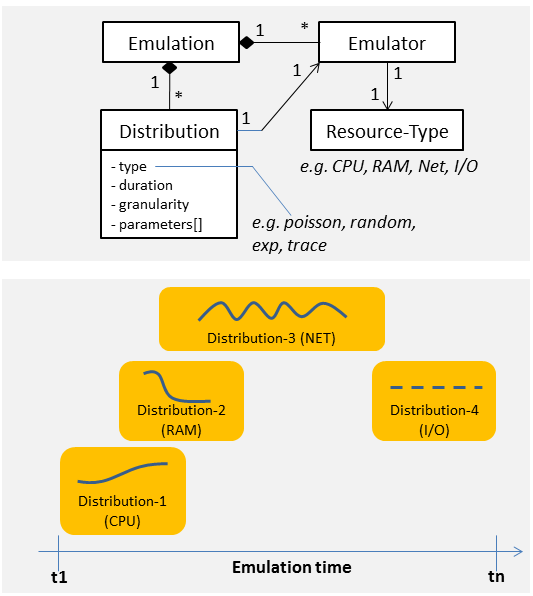
\includegraphics{emulation2.png}
\end{figure}
\end{quote}


\subsection{Getting Started}
\label{COCOMA/02_how_to_use_it:getting-started}\label{COCOMA/02_how_to_use_it::doc}
COCOMA is installed in \emph{``/usr/share/pyshared/cocoma''}. In this section we provide information about the components that have to be running in order to fully use the framework, and how can a user interact with it.


\subsubsection{Starting Components}
\label{COCOMA/02_how_to_use_it:starting-components}
The two main components of COCOMA are:
\begin{itemize}
\item {} 
Scheduler daemon (mandatory, needs to be the first started)

\item {} 
API Daemon (optional, if the REST API functionality is required)

\end{itemize}

The \textbf{Scheduler daemon} - runs in the background and executes workload with differential parameters at the time defined in the emulation properties.
To check if the scheduler is running use the following:

\begin{Verbatim}[commandchars=\\\{\}]
\PYG{n+nv}{\PYGZdl{} }ccmsh \PYGZhy{}\PYGZhy{}show scheduler
\end{Verbatim}

To start the scheduler on a specific network interface and port, use the command:

\begin{Verbatim}[commandchars=\\\{\}]
\PYG{n+nv}{\PYGZdl{} }ccmsh \PYGZhy{}\PYGZhy{}start scheduler eth1 55555
\end{Verbatim}

If the network interface and port are omitted, the default values are respectively \emph{eth0} adn \emph{51889}

If more detailed output information is needed, the \emph{Scheduler} can also be started in \emph{DEBUG} mode:

\begin{Verbatim}[commandchars=\\\{\}]
\PYG{n+nv}{\PYGZdl{} }ccmsh \PYGZhy{}\PYGZhy{}start scheduler eth1 55555 debug
\end{Verbatim}

The \textbf{API daemon} - provides the RESTfull web API, which exposes COCOMA resources to be used over the network. It follows the same command structure as the Scheduler.
To check if the scheduler is running use the following:

\begin{Verbatim}[commandchars=\\\{\}]
\PYG{n+nv}{\PYGZdl{} }ccmsh \PYGZhy{}\PYGZhy{}show api
\end{Verbatim}

To start the api on a specific network interface and port, use the command:

\begin{Verbatim}[commandchars=\\\{\}]
\PYG{n+nv}{\PYGZdl{} }ccmsh \PYGZhy{}\PYGZhy{}start api eth2 77777
\end{Verbatim}

If the network interface and port are omitted, the default values are respectively \emph{eth0} and \emph{5050}

The log level is the same specified for the \emph{Scheduler}.


\subsubsection{CLI}
\label{COCOMA/02_how_to_use_it:cli}
The COCOMA CLI is called \emph{ccmsh}, and provides the following options:
\index{ccmsh command line option!-h, --help}\index{-h, --help!ccmsh command line option}

\begin{fulllineitems}
\phantomsection\label{COCOMA/02_how_to_use_it:cmdoption-ccmsh-h}\pysigline{\bfcode{-h}\code{}\code{,~}\bfcode{-{-}help}\code{}}
Display help information of the available options

\end{fulllineitems}

\index{ccmsh command line option!-v, --version}\index{-v, --version!ccmsh command line option}

\begin{fulllineitems}
\phantomsection\label{COCOMA/02_how_to_use_it:cmdoption-ccmsh-v}\pysigline{\bfcode{-v}\code{}\code{,~}\bfcode{-{-}version}\code{}}
Display installed version information of COCOMA

\end{fulllineitems}

\index{ccmsh command line option!-q, --mq}\index{-q, --mq!ccmsh command line option}

\begin{fulllineitems}
\phantomsection\label{COCOMA/02_how_to_use_it:cmdoption-ccmsh-q}\pysigline{\bfcode{-q}\code{}\code{,~}\bfcode{-{-}mq}\code{}}
add configuration parameters for message queue:
enabled vhost exchange user password host topic

\end{fulllineitems}

\index{ccmsh command line option!-m, --rmq}\index{-m, --rmq!ccmsh command line option}

\begin{fulllineitems}
\phantomsection\label{COCOMA/02_how_to_use_it:cmdoption-ccmsh-m}\pysigline{\bfcode{-m}\code{}\code{,~}\bfcode{-{-}rmq}\code{}}
remove configuration parameters for message queue

\end{fulllineitems}

\index{ccmsh command line option!-a, --enl}\index{-a, --enl!ccmsh command line option}

\begin{fulllineitems}
\phantomsection\label{COCOMA/02_how_to_use_it:cmdoption-ccmsh-a}\pysigline{\bfcode{-a}\code{}\code{,~}\bfcode{-{-}enl}\code{}}
enable configuration parameters for message queue

\end{fulllineitems}

\index{ccmsh command line option!-s, --smq}\index{-s, --smq!ccmsh command line option}

\begin{fulllineitems}
\phantomsection\label{COCOMA/02_how_to_use_it:cmdoption-ccmsh-s}\pysigline{\bfcode{-s}\code{}\code{,~}\bfcode{-{-}smq}\code{}}
show configuration parameters for message queue

\end{fulllineitems}

\index{ccmsh command line option!-b, --bfz}\index{-b, --bfz!ccmsh command line option}

\begin{fulllineitems}
\phantomsection\label{COCOMA/02_how_to_use_it:cmdoption-ccmsh-b}\pysigline{\bfcode{-b}\code{}\code{,~}\bfcode{-{-}bfz}\code{}}
Update the path of to the backfuzz emulator (stored in database)

\end{fulllineitems}

\index{ccmsh command line option!-l, --list \textless{}emulation name\textgreater{}}\index{-l, --list \textless{}emulation name\textgreater{}!ccmsh command line option}

\begin{fulllineitems}
\phantomsection\label{COCOMA/02_how_to_use_it:cmdoption-ccmsh-l}\pysigline{\bfcode{-l}\code{}\code{,~}\bfcode{-{-}list}\code{~\textless{}emulation~name\textgreater{}}}
Display list of all emulations that are scheduled or already finished. If emulation name is provided then it lists information for that specific emulation

\end{fulllineitems}

\index{ccmsh command line option!-r, --results \textless{}emulation name\textgreater{}}\index{-r, --results \textless{}emulation name\textgreater{}!ccmsh command line option}

\begin{fulllineitems}
\phantomsection\label{COCOMA/02_how_to_use_it:cmdoption-ccmsh-r}\pysigline{\bfcode{-r}\code{}\code{,~}\bfcode{-{-}results}\code{~\textless{}emulation~name\textgreater{}}}
Display list of results of all emulations that are scheduled or already finished. If emulation name is provided, then it lists information for that specific emulation

\end{fulllineitems}

\index{ccmsh command line option!-j, --list-jobs}\index{-j, --list-jobs!ccmsh command line option}

\begin{fulllineitems}
\phantomsection\label{COCOMA/02_how_to_use_it:cmdoption-ccmsh-j}\pysigline{\bfcode{-j}\code{}\code{,~}\bfcode{-{-}list-jobs}\code{}}
Queries the scheduler for the list of jobs that are scheduled to be executed and are currently executing. For each one, it gives the job name and the planned execution time

\end{fulllineitems}

\index{ccmsh command line option!-i, --dist \textless{}distribution name\textgreater{}}\index{-i, --dist \textless{}distribution name\textgreater{}!ccmsh command line option}

\begin{fulllineitems}
\phantomsection\label{COCOMA/02_how_to_use_it:cmdoption-ccmsh-i}\pysigline{\bfcode{-i}\code{}\code{,~}\bfcode{-{-}dist}\code{~\textless{}distribution~name\textgreater{}}}
Scans the \emph{``/usr/share/pyshared/cocoma/distributions''} folder and displays all available distribution modules. If a distribution name is provided, then it shows the help information for that specific distribution

\end{fulllineitems}

\index{ccmsh command line option!-e, --emu \textless{}emulator name\textgreater{}}\index{-e, --emu \textless{}emulator name\textgreater{}!ccmsh command line option}

\begin{fulllineitems}
\phantomsection\label{COCOMA/02_how_to_use_it:cmdoption-ccmsh-e}\pysigline{\bfcode{-e}\code{}\code{,~}\bfcode{-{-}emu}\code{~\textless{}emulator~name\textgreater{}}}
Scans the \emph{``/usr/share/pyshared/cocoma/emulators''} folder and displays all available emulator wrapper modules. If an emulator name is provided, then it shows the help information for that specific emulator wrapper

\end{fulllineitems}

\index{ccmsh command line option!-x, --xml \textless{}file name\textgreater{}}\index{-x, --xml \textless{}file name\textgreater{}!ccmsh command line option}

\begin{fulllineitems}
\phantomsection\label{COCOMA/02_how_to_use_it:cmdoption-ccmsh-x}\pysigline{\bfcode{-x}\code{}\code{,~}\bfcode{-{-}xml}\code{~\textless{}file~name\textgreater{}}}
It create and emulation based on the local XML

\end{fulllineitems}

\index{ccmsh command line option!-n, --now (used with -x option only)}\index{-n, --now (used with -x option only)!ccmsh command line option}

\begin{fulllineitems}
\phantomsection\label{COCOMA/02_how_to_use_it:cmdoption-ccmsh-n}\pysigline{\bfcode{-n}\code{}\code{,~}\bfcode{-{-}now}\code{~(used~with~-x~option~only)}}
Override any start date in the local XML emulation file without modifying the file, i.e. \code{ccmsh -x \textless{}file name\textgreater{} -n}

\end{fulllineitems}

\index{ccmsh command line option!-d, --delete \textless{}emulation name\textgreater{}}\index{-d, --delete \textless{}emulation name\textgreater{}!ccmsh command line option}

\begin{fulllineitems}
\phantomsection\label{COCOMA/02_how_to_use_it:cmdoption-ccmsh-d}\pysigline{\bfcode{-d}\code{}\code{,~}\bfcode{-{-}delete}\code{~\textless{}emulation~name\textgreater{}}}
Deletes a specific emulation from the database

\end{fulllineitems}

\index{ccmsh command line option!-p, --purge}\index{-p, --purge!ccmsh command line option}

\begin{fulllineitems}
\phantomsection\label{COCOMA/02_how_to_use_it:cmdoption-ccmsh-p}\pysigline{\bfcode{-p}\code{}\code{,~}\bfcode{-{-}purge}\code{}}
Remove all DB entries, all scheduled jobs

\end{fulllineitems}

\index{ccmsh command line option!--start \textless{}api interface port\textgreater{}, \textless{}scheduler interface port\textgreater{}}\index{--start \textless{}api interface port\textgreater{}, \textless{}scheduler interface port\textgreater{}!ccmsh command line option}

\begin{fulllineitems}
\phantomsection\label{COCOMA/02_how_to_use_it:cmdoption-ccmsh--start}\pysigline{\bfcode{-{-}start}\code{~\textless{}api~interface~port\textgreater{},~\textless{}scheduler~interface~port\textgreater{}}}
Start Scheduler or API daemon by specifying network interface and port number i.e. \code{ccmsh -{-}start api eth0 2020} or \code{ccmsh -{-}start scheduler eth0 3030}. By default if the network interface is not specified, the Scheduler daemon will run on \emph{eth0} and \emph{51889}, and the API daemon will run on \emph{eth0} and \emph{5050}.

\end{fulllineitems}

\index{ccmsh command line option!--stop \textless{}api\textgreater{}, \textless{}scheduler\textgreater{}}\index{--stop \textless{}api\textgreater{}, \textless{}scheduler\textgreater{}!ccmsh command line option}

\begin{fulllineitems}
\phantomsection\label{COCOMA/02_how_to_use_it:cmdoption-ccmsh--stop}\pysigline{\bfcode{-{-}stop}\code{~\textless{}api\textgreater{},~\textless{}scheduler\textgreater{}}}
Stop Scheduler or API daemon

\end{fulllineitems}

\index{ccmsh command line option!--show \textless{}api\textgreater{}, \textless{}scheduler\textgreater{}}\index{--show \textless{}api\textgreater{}, \textless{}scheduler\textgreater{}!ccmsh command line option}

\begin{fulllineitems}
\phantomsection\label{COCOMA/02_how_to_use_it:cmdoption-ccmsh--show}\pysigline{\bfcode{-{-}show}\code{~\textless{}api\textgreater{},~\textless{}scheduler\textgreater{}}}
Show OS information on Scheduler or API daemon, displays PID numbers

\end{fulllineitems}



\subsubsection{Logging}
\label{COCOMA/02_how_to_use_it:logging}

\paragraph{Event Logging}
\label{COCOMA/02_how_to_use_it:event-logging}
COCOMA provides two levels of event logging, \emph{INFO} which is set by default, and \emph{DEBUG} which can be enabled if more detailed feedback is required:

\begin{Verbatim}[commandchars=\\\{\}]
\PYG{n+nv}{\PYGZdl{} }ccmsh \PYGZhy{}\PYGZhy{}start scheduler eth1 55555 debug
\end{Verbatim}

Timestamped events are then saved in the \code{logs/COCOMAlogfile.csv} file.

Both \emph{Scheduler} and \emph{API} also save their CLI output in the \code{logs/COCOMAlogfile\_Scheduler\_sout.txt} and \code{logs/COCOMAlogfile\_API\_sout.txt} accordingly.
All above files can be retrieved as ZIP archive through COCOMA web API URI:

\begin{Verbatim}[commandchars=\\\{\}]
* /logs/system
\end{Verbatim}


\paragraph{Resource Consumption Logging}
\label{COCOMA/02_how_to_use_it:resource-consumption-logging}
Optionally the CPU, Memory and Network consumption of COCOMA VM can be recorded during each emulation. To enable resource consumption logging just add this XML code block to the payload:

\begin{Verbatim}[commandchars=\\\{\}]
\PYG{n+nt}{\PYGZlt{}log}\PYG{n+nt}{\PYGZgt{}}
 \PYG{c}{\PYGZlt{}!\PYGZhy{}\PYGZhy{}}\PYG{c}{ Use value \PYGZdq{}1\PYGZdq{} to enable logging(by default logging is off)  }\PYG{c}{\PYGZhy{}\PYGZhy{}\PYGZgt{}}
 \PYG{n+nt}{\PYGZlt{}enable}\PYG{n+nt}{\PYGZgt{}}1\PYG{n+nt}{\PYGZlt{}/enable\PYGZgt{}}
 \PYG{c}{\PYGZlt{}!\PYGZhy{}\PYGZhy{}}\PYG{c}{ Use seconds for setting probe intervals(if logging is enabled default is 3sec)  }\PYG{c}{\PYGZhy{}\PYGZhy{}\PYGZgt{}}
 \PYG{n+nt}{\PYGZlt{}frequency}\PYG{n+nt}{\PYGZgt{}}1\PYG{n+nt}{\PYGZlt{}/frequency\PYGZgt{}}
 \PYG{c}{\PYGZlt{}!\PYGZhy{}\PYGZhy{}}\PYG{c}{ Set the level of information detail  }\PYG{c}{\PYGZhy{}\PYGZhy{}\PYGZgt{}}
 \PYG{n+nt}{\PYGZlt{}logLevel}\PYG{n+nt}{\PYGZgt{}}debug\PYG{n+nt}{\PYGZlt{}/logLevel\PYGZgt{}}
\PYG{n+nt}{\PYGZlt{}/log\PYGZgt{}}
\end{Verbatim}

If the logging was enabled, once the emulation is finished, COCOMA will produce two files named after the emulation (e.g. \code{logs/4-CPU\_EMU-res\_2013-04-09T18:51:09.csv} and \code{logs/4-CPU\_EMU-config\_2013-04-09T18:51:09.xml}).
The file with CSV extention will contain the system resource data, and the file with XML extention will have the exact copy of the payload used for that emulation.

Both files can be retrieved as ZIP archive through COCOMA web API URI by emulation name:

\begin{Verbatim}[commandchars=\\\{\}]
* /logs/emulations
* /logs/emulations/\PYGZob{}name\PYGZcb{}
\end{Verbatim}


\subsubsection{REST API}
\label{COCOMA/02_how_to_use_it:rest-api}

\paragraph{Index}
\label{COCOMA/02_how_to_use_it:index}
The API URIs summary list is as follow:

\begin{Verbatim}[commandchars=\\\{\}]
* /
* /emulations
* /emulations/\PYGZob{}name\PYGZcb{}
* /distributions
* /distributions/\PYGZob{}name\PYGZcb{}
* /emulators
* /emulators/\PYGZob{}name\PYGZcb{}
* /results
* /results/\PYGZob{}name\PYGZcb{}
* /tests
* /tests/\PYGZob{}name\PYGZcb{}
* /logs
* /logs/system
* /logs/emulations
* /logs/emulations/\PYGZob{}name\PYGZcb{}
\end{Verbatim}


\paragraph{Description}
\label{COCOMA/02_how_to_use_it:description}
\code{http:method:: GET /}
\begin{quote}

The \textbf{root} returns a \emph{collection} of all the available resources. Example of a XML response:

\begin{Verbatim}[commandchars=\\\{\}]
\PYG{c+cp}{\PYGZlt{}?xml version=\PYGZdq{}1.0\PYGZdq{} ?\PYGZgt{}}
\PYG{n+nt}{\PYGZlt{}root} \PYG{n+na}{href=}\PYG{l+s}{\PYGZdq{}/\PYGZdq{}}\PYG{n+nt}{\PYGZgt{}}
        \PYG{n+nt}{\PYGZlt{}version}\PYG{n+nt}{\PYGZgt{}}0.1.1\PYG{n+nt}{\PYGZlt{}/version\PYGZgt{}}
        \PYG{n+nt}{\PYGZlt{}timestamp}\PYG{n+nt}{\PYGZgt{}}1365518303.44\PYG{n+nt}{\PYGZlt{}/timestamp\PYGZgt{}}
        \PYG{n+nt}{\PYGZlt{}link} \PYG{n+na}{href=}\PYG{l+s}{\PYGZdq{}/emulations\PYGZdq{}} \PYG{n+na}{rel=}\PYG{l+s}{\PYGZdq{}emulations\PYGZdq{}} \PYG{n+na}{type=}\PYG{l+s}{\PYGZdq{}application/vnd.bonfire+xml\PYGZdq{}}\PYG{n+nt}{/\PYGZgt{}}
        \PYG{n+nt}{\PYGZlt{}link} \PYG{n+na}{href=}\PYG{l+s}{\PYGZdq{}/emulators\PYGZdq{}} \PYG{n+na}{rel=}\PYG{l+s}{\PYGZdq{}emulators\PYGZdq{}} \PYG{n+na}{type=}\PYG{l+s}{\PYGZdq{}application/vnd.bonfire+xml\PYGZdq{}}\PYG{n+nt}{/\PYGZgt{}}
        \PYG{n+nt}{\PYGZlt{}link} \PYG{n+na}{href=}\PYG{l+s}{\PYGZdq{}/distributions\PYGZdq{}} \PYG{n+na}{rel=}\PYG{l+s}{\PYGZdq{}distributions\PYGZdq{}} \PYG{n+na}{type=}\PYG{l+s}{\PYGZdq{}application/vnd.bonfire+xml\PYGZdq{}}\PYG{n+nt}{/\PYGZgt{}}
        \PYG{n+nt}{\PYGZlt{}link} \PYG{n+na}{href=}\PYG{l+s}{\PYGZdq{}/tests\PYGZdq{}} \PYG{n+na}{rel=}\PYG{l+s}{\PYGZdq{}tests\PYGZdq{}} \PYG{n+na}{type=}\PYG{l+s}{\PYGZdq{}application/vnd.bonfire+xml\PYGZdq{}}\PYG{n+nt}{/\PYGZgt{}}
        \PYG{n+nt}{\PYGZlt{}link} \PYG{n+na}{href=}\PYG{l+s}{\PYGZdq{}/results\PYGZdq{}} \PYG{n+na}{rel=}\PYG{l+s}{\PYGZdq{}results\PYGZdq{}} \PYG{n+na}{type=}\PYG{l+s}{\PYGZdq{}application/vnd.bonfire+xml\PYGZdq{}}\PYG{n+nt}{/\PYGZgt{}}
        \PYG{n+nt}{\PYGZlt{}link} \PYG{n+na}{href=}\PYG{l+s}{\PYGZdq{}/logs\PYGZdq{}} \PYG{n+na}{rel=}\PYG{l+s}{\PYGZdq{}logs\PYGZdq{}} \PYG{n+na}{type=}\PYG{l+s}{\PYGZdq{}application/vnd.bonfire+xml\PYGZdq{}}\PYG{n+nt}{/\PYGZgt{}}
\PYG{n+nt}{\PYGZlt{}/root\PYGZgt{}}
\end{Verbatim}
\end{quote}

\code{http:method:: GET /emulations}
\begin{quote}

The \textbf{emulations} returns a \emph{collection} of all the available emulation resources. Example of a XML response:

\begin{Verbatim}[commandchars=\\\{\}]
\PYG{c+cp}{\PYGZlt{}?xml version=\PYGZdq{}1.0\PYGZdq{} ?\PYGZgt{}}
\PYG{n+nt}{\PYGZlt{}collection} \PYG{n+na}{href=}\PYG{l+s}{\PYGZdq{}/emulations\PYGZdq{}} \PYG{n+na}{xmlns=}\PYG{l+s}{\PYGZdq{}http://127.0.0.1/cocoma\PYGZdq{}}\PYG{n+nt}{\PYGZgt{}}
        \PYG{n+nt}{\PYGZlt{}items} \PYG{n+na}{offset=}\PYG{l+s}{\PYGZdq{}0\PYGZdq{}} \PYG{n+na}{total=}\PYG{l+s}{\PYGZdq{}3\PYGZdq{}}\PYG{n+nt}{\PYGZgt{}}
                \PYG{n+nt}{\PYGZlt{}emulation} \PYG{n+na}{href=}\PYG{l+s}{\PYGZdq{}/emulations/1\PYGZhy{}Emu\PYGZhy{}CPU\PYGZhy{}RAM\PYGZhy{}IO\PYGZdq{}} \PYG{n+na}{id=}\PYG{l+s}{\PYGZdq{}1\PYGZdq{}} \PYG{n+na}{name=}\PYG{l+s}{\PYGZdq{}1\PYGZhy{}Emu\PYGZhy{}CPU\PYGZhy{}RAM\PYGZhy{}IO\PYGZdq{}} \PYG{n+na}{state=}\PYG{l+s}{\PYGZdq{}inactive\PYGZdq{}}\PYG{n+nt}{/\PYGZgt{}}
                \PYG{n+nt}{\PYGZlt{}emulation} \PYG{n+na}{href=}\PYG{l+s}{\PYGZdq{}/emulations/2\PYGZhy{}CPU\PYGZus{}EMU\PYGZdq{}} \PYG{n+na}{id=}\PYG{l+s}{\PYGZdq{}2\PYGZdq{}} \PYG{n+na}{name=}\PYG{l+s}{\PYGZdq{}2\PYGZhy{}CPU\PYGZus{}EMU\PYGZdq{}} \PYG{n+na}{state=}\PYG{l+s}{\PYGZdq{}inactive\PYGZdq{}}\PYG{n+nt}{/\PYGZgt{}}
                \PYG{n+nt}{\PYGZlt{}emulation} \PYG{n+na}{href=}\PYG{l+s}{\PYGZdq{}/emulations/3\PYGZhy{}CPU\PYGZus{}EMU\PYGZdq{}} \PYG{n+na}{id=}\PYG{l+s}{\PYGZdq{}3\PYGZdq{}} \PYG{n+na}{name=}\PYG{l+s}{\PYGZdq{}3\PYGZhy{}CPU\PYGZus{}EMU\PYGZdq{}} \PYG{n+na}{state=}\PYG{l+s}{\PYGZdq{}inactive\PYGZdq{}}\PYG{n+nt}{/\PYGZgt{}}
        \PYG{n+nt}{\PYGZlt{}/items\PYGZgt{}}
        \PYG{n+nt}{\PYGZlt{}link} \PYG{n+na}{href=}\PYG{l+s}{\PYGZdq{}/\PYGZdq{}} \PYG{n+na}{rel=}\PYG{l+s}{\PYGZdq{}parent\PYGZdq{}} \PYG{n+na}{type=}\PYG{l+s}{\PYGZdq{}application/vnd.bonfire+xml\PYGZdq{}}\PYG{n+nt}{/\PYGZgt{}}
\PYG{n+nt}{\PYGZlt{}/collection\PYGZgt{}}
\end{Verbatim}
\end{quote}

\code{http:method:: GET /emulations/\{name\}}
\begin{quote}

Displays information about emulation by name. The returned \emph{200-OK} XML is:

\begin{Verbatim}[commandchars=\\\{\}]
\PYG{c+cp}{\PYGZlt{}?xml version=\PYGZdq{}1.0\PYGZdq{} ?\PYGZgt{}}
\PYG{n+nt}{\PYGZlt{}emulation} \PYG{n+na}{href=}\PYG{l+s}{\PYGZdq{}/emulations/1\PYGZhy{}Emu\PYGZhy{}CPU\PYGZhy{}RAM\PYGZhy{}IO\PYGZdq{}} \PYG{n+na}{xmlns=}\PYG{l+s}{\PYGZdq{}http://127.0.0.1/cocoma\PYGZdq{}}\PYG{n+nt}{\PYGZgt{}}
        \PYG{n+nt}{\PYGZlt{}id}\PYG{n+nt}{\PYGZgt{}}1\PYG{n+nt}{\PYGZlt{}/id\PYGZgt{}}
        \PYG{n+nt}{\PYGZlt{}emulationName}\PYG{n+nt}{\PYGZgt{}}1\PYGZhy{}Emu\PYGZhy{}CPU\PYGZhy{}RAM\PYGZhy{}IO\PYG{n+nt}{\PYGZlt{}/emulationName\PYGZgt{}}
        \PYG{n+nt}{\PYGZlt{}emulationType}\PYG{n+nt}{\PYGZgt{}}mix\PYG{n+nt}{\PYGZlt{}/emulationType\PYGZgt{}}
        \PYG{n+nt}{\PYGZlt{}resourceType}\PYG{n+nt}{\PYGZgt{}}mix\PYG{n+nt}{\PYGZlt{}/resourceType\PYGZgt{}}
        \PYG{n+nt}{\PYGZlt{}emuStartTime}\PYG{n+nt}{\PYGZgt{}}2013\PYGZhy{}04\PYGZhy{}09T13:00:01\PYG{n+nt}{\PYGZlt{}/emuStartTime\PYGZgt{}}
        \PYG{n+nt}{\PYGZlt{}emuStopTime}\PYG{n+nt}{\PYGZgt{}}180\PYG{n+nt}{\PYGZlt{}/emuStopTime\PYGZgt{}}
        \PYG{n+nt}{\PYGZlt{}scheduledJobs}\PYG{n+nt}{\PYGZgt{}}
                \PYG{n+nt}{\PYGZlt{}jobsempty}\PYG{n+nt}{\PYGZgt{}}No jobs are scheduled\PYG{n+nt}{\PYGZlt{}/jobsempty\PYGZgt{}}
        \PYG{n+nt}{\PYGZlt{}/scheduledJobs\PYGZgt{}}
        \PYG{n+nt}{\PYGZlt{}distributions} \PYG{n+na}{ID=}\PYG{l+s}{\PYGZdq{}1\PYGZdq{}} \PYG{n+na}{name=}\PYG{l+s}{\PYGZdq{}Distro1\PYGZdq{}}\PYG{n+nt}{\PYGZgt{}}
                \PYG{n+nt}{\PYGZlt{}startTime}\PYG{n+nt}{\PYGZgt{}}5\PYG{n+nt}{\PYGZlt{}/startTime\PYGZgt{}}
                \PYG{n+nt}{\PYGZlt{}granularity}\PYG{n+nt}{\PYGZgt{}}3\PYG{n+nt}{\PYGZlt{}/granularity\PYGZgt{}}
                \PYG{n+nt}{\PYGZlt{}duration}\PYG{n+nt}{\PYGZgt{}}30\PYG{n+nt}{\PYGZlt{}/duration\PYGZgt{}}
                \PYG{n+nt}{\PYGZlt{}startload}\PYG{n+nt}{\PYGZgt{}}10\PYG{n+nt}{\PYGZlt{}/startload\PYGZgt{}}
                \PYG{n+nt}{\PYGZlt{}stopload}\PYG{n+nt}{\PYGZgt{}}90\PYG{n+nt}{\PYGZlt{}/stopload\PYGZgt{}}
        \PYG{n+nt}{\PYGZlt{}/distributions\PYGZgt{}}
        \PYG{n+nt}{\PYGZlt{}distributions} \PYG{n+na}{ID=}\PYG{l+s}{\PYGZdq{}2\PYGZdq{}} \PYG{n+na}{name=}\PYG{l+s}{\PYGZdq{}Distro2\PYGZdq{}}\PYG{n+nt}{\PYGZgt{}}
                \PYG{n+nt}{\PYGZlt{}startTime}\PYG{n+nt}{\PYGZgt{}}5\PYG{n+nt}{\PYGZlt{}/startTime\PYGZgt{}}
                \PYG{n+nt}{\PYGZlt{}granularity}\PYG{n+nt}{\PYGZgt{}}3\PYG{n+nt}{\PYGZlt{}/granularity\PYGZgt{}}
                \PYG{n+nt}{\PYGZlt{}duration}\PYG{n+nt}{\PYGZgt{}}30\PYG{n+nt}{\PYGZlt{}/duration\PYGZgt{}}
                \PYG{n+nt}{\PYGZlt{}startload}\PYG{n+nt}{\PYGZgt{}}10\PYG{n+nt}{\PYGZlt{}/startload\PYGZgt{}}
                \PYG{n+nt}{\PYGZlt{}stopload}\PYG{n+nt}{\PYGZgt{}}90\PYG{n+nt}{\PYGZlt{}/stopload\PYGZgt{}}
        \PYG{n+nt}{\PYGZlt{}/distributions\PYGZgt{}}
        \PYG{n+nt}{\PYGZlt{}link} \PYG{n+na}{href=}\PYG{l+s}{\PYGZdq{}/\PYGZdq{}} \PYG{n+na}{rel=}\PYG{l+s}{\PYGZdq{}parent\PYGZdq{}} \PYG{n+na}{type=}\PYG{l+s}{\PYGZdq{}application/vnd.bonfire+xml\PYGZdq{}}\PYG{n+nt}{/\PYGZgt{}}
        \PYG{n+nt}{\PYGZlt{}link} \PYG{n+na}{href=}\PYG{l+s}{\PYGZdq{}/emulations\PYGZdq{}} \PYG{n+na}{rel=}\PYG{l+s}{\PYGZdq{}parent\PYGZdq{}} \PYG{n+na}{type=}\PYG{l+s}{\PYGZdq{}application/vnd.bonfire+xml\PYGZdq{}}\PYG{n+nt}{/\PYGZgt{}}
\PYG{n+nt}{\PYGZlt{}/emulation\PYGZgt{}}
\end{Verbatim}

The returned \emph{404 – Not Found} XML is:

\begin{Verbatim}[commandchars=\\\{\}]
\PYG{n+nt}{\PYGZlt{}error}\PYG{n+nt}{\PYGZgt{}}Emulation Name: 1\PYGZhy{}Emu\PYGZhy{}CPU\PYGZhy{}RAM\PYGZhy{}IO1 not found. Error:too many values to unpack\PYG{n+nt}{\PYGZlt{}/error\PYGZgt{}}
\end{Verbatim}
\end{quote}

\code{http:method:: POST /emulations}
\begin{quote}

\begin{Verbatim}[commandchars=\\\{\}]
:param string XML: Emulation parameters defined via XML as shown in the examples section.
\end{Verbatim}

The returned \emph{201-Created} XML:

\begin{Verbatim}[commandchars=\\\{\}]
\PYG{c+cp}{\PYGZlt{}?xml version=\PYGZdq{}1.0\PYGZdq{} ?\PYGZgt{}}
\PYG{n+nt}{\PYGZlt{}emulation} \PYG{n+na}{href=}\PYG{l+s}{\PYGZdq{}/emulations/4\PYGZhy{}CPU\PYGZus{}EMU\PYGZdq{}} \PYG{n+na}{xmlns=}\PYG{l+s}{\PYGZdq{}http://127.0.0.1/cocoma\PYGZdq{}}\PYG{n+nt}{\PYGZgt{}}
        \PYG{n+nt}{\PYGZlt{}ID}\PYG{n+nt}{\PYGZgt{}}4\PYGZhy{}CPU\PYGZus{}EMU\PYG{n+nt}{\PYGZlt{}/ID\PYGZgt{}}
        \PYG{n+nt}{\PYGZlt{}EmuNotes}\PYG{n+nt}{\PYGZgt{}}OK\PYG{n+nt}{\PYGZlt{}/EmuNotes\PYGZgt{}}
        \PYG{n+nt}{\PYGZlt{}DistroNotes}\PYG{n+nt}{\PYGZgt{}}OK\PYG{n+nt}{\PYGZlt{}/DistroNotes\PYGZgt{}}
        \PYG{n+nt}{\PYGZlt{}link} \PYG{n+na}{href=}\PYG{l+s}{\PYGZdq{}/\PYGZdq{}} \PYG{n+na}{rel=}\PYG{l+s}{\PYGZdq{}parent\PYGZdq{}} \PYG{n+na}{type=}\PYG{l+s}{\PYGZdq{}application/vnd.bonfire+xml\PYGZdq{}}\PYG{n+nt}{/\PYGZgt{}}
        \PYG{n+nt}{\PYGZlt{}link} \PYG{n+na}{href=}\PYG{l+s}{\PYGZdq{}/emulations\PYGZdq{}} \PYG{n+na}{rel=}\PYG{l+s}{\PYGZdq{}parent\PYGZdq{}} \PYG{n+na}{type=}\PYG{l+s}{\PYGZdq{}application/vnd.bonfire+xml\PYGZdq{}}\PYG{n+nt}{/\PYGZgt{}}
\PYG{n+nt}{\PYGZlt{}/emulation\PYGZgt{}}
\end{Verbatim}

The returned \emph{400 – Bad Request} XML:

\begin{Verbatim}[commandchars=\\\{\}]
\PYG{c+cp}{\PYGZlt{}?xml version=\PYGZdq{}1.0\PYGZdq{} ?\PYGZgt{}}
\PYG{n+nt}{\PYGZlt{}error}\PYG{n+nt}{\PYGZgt{}}XML is not well formed Error: syntax error: line 1, column 0\PYG{n+nt}{\PYGZlt{}/error\PYGZgt{}}
\end{Verbatim}
\end{quote}

\code{http:method:: GET /emulators}
\begin{quote}

Displays emulators list. The returned \emph{200- OK} XML:

\begin{Verbatim}[commandchars=\\\{\}]
\PYG{c+cp}{\PYGZlt{}?xml version=\PYGZdq{}1.0\PYGZdq{} ?\PYGZgt{}}
\PYG{n+nt}{\PYGZlt{}collection} \PYG{n+na}{href=}\PYG{l+s}{\PYGZdq{}/emulators\PYGZdq{}} \PYG{n+na}{xmlns=}\PYG{l+s}{\PYGZdq{}http://127.0.0.1/cocoma\PYGZdq{}}\PYG{n+nt}{\PYGZgt{}}
        \PYG{n+nt}{\PYGZlt{}items} \PYG{n+na}{offset=}\PYG{l+s}{\PYGZdq{}0\PYGZdq{}} \PYG{n+na}{total=}\PYG{l+s}{\PYGZdq{}3\PYGZdq{}}\PYG{n+nt}{\PYGZgt{}}
                \PYG{n+nt}{\PYGZlt{}emulator} \PYG{n+na}{href=}\PYG{l+s}{\PYGZdq{}/emulators/lookbusy\PYGZdq{}} \PYG{n+na}{name=}\PYG{l+s}{\PYGZdq{}lookbusy\PYGZdq{}}\PYG{n+nt}{/\PYGZgt{}}
                \PYG{n+nt}{\PYGZlt{}emulator} \PYG{n+na}{href=}\PYG{l+s}{\PYGZdq{}/emulators/stressapptest\PYGZdq{}} \PYG{n+na}{name=}\PYG{l+s}{\PYGZdq{}stressapptest\PYGZdq{}}\PYG{n+nt}{/\PYGZgt{}}
                \PYG{n+nt}{\PYGZlt{}emulator} \PYG{n+na}{href=}\PYG{l+s}{\PYGZdq{}/emulators/iperf\PYGZdq{}} \PYG{n+na}{name=}\PYG{l+s}{\PYGZdq{}iperf\PYGZdq{}}\PYG{n+nt}{/\PYGZgt{}}
        \PYG{n+nt}{\PYGZlt{}/items\PYGZgt{}}
        \PYG{n+nt}{\PYGZlt{}link} \PYG{n+na}{href=}\PYG{l+s}{\PYGZdq{}/\PYGZdq{}} \PYG{n+na}{rel=}\PYG{l+s}{\PYGZdq{}parent\PYGZdq{}} \PYG{n+na}{type=}\PYG{l+s}{\PYGZdq{}application/vnd.bonfire+xml\PYGZdq{}}\PYG{n+nt}{/\PYGZgt{}}
\PYG{n+nt}{\PYGZlt{}/collection\PYGZgt{}}
\end{Verbatim}
\end{quote}

\code{http:method:: GET /emulators/\{name\}}
\begin{quote}

\begin{Verbatim}[commandchars=\\\{\}]
:arg name: Name of emulator that you want to get more info
\end{Verbatim}

Displays information about emulator by name. It returns parameters that can be used with emulator and the values limits (where applicable). The returned \emph{200- OK} XML:

\begin{Verbatim}[commandchars=\\\{\}]
\PYG{c+cp}{\PYGZlt{}?xml version=\PYGZdq{}1.0\PYGZdq{} ?\PYGZgt{}}
\PYG{n+nt}{\PYGZlt{}emulator} \PYG{n+na}{href=}\PYG{l+s}{\PYGZdq{}/emulators/lookbusy\PYGZdq{}} \PYG{n+na}{xmlns=}\PYG{l+s}{\PYGZdq{}http://127.0.0.1/cocoma\PYGZdq{}}\PYG{n+nt}{\PYGZgt{}}
  \PYG{n+nt}{\PYGZlt{}info}\PYG{n+nt}{\PYGZgt{}}
    \PYG{n+nt}{\PYGZlt{}help}\PYG{n+nt}{\PYGZgt{}}
    Emulator lookbusy can be used for following resources:
    1)Loads CPU with parameters:
      ncpus \PYGZhy{} Number of CPUs to keep busy (default: autodetected)

    2)Loads Memory(MEM) with parameters:
      memSleep \PYGZhy{} Time to sleep between iterations, in usec (default 1000)

    3)Changing size of files to use during IO with parameters:
      ioBlockSize \PYGZhy{} Size of blocks to use for I/O in MB
      ioSleep \PYGZhy{} Time to sleep between iterations, in msec (default 100)


    XML block example:
    \PYG{n+ni}{\PYGZam{}lt;}emulator\PYGZhy{}params\PYG{n+ni}{\PYGZam{}gt;}
        \PYG{n+ni}{\PYGZam{}lt;}resourceType\PYG{n+ni}{\PYGZam{}gt;}CPU\PYG{n+ni}{\PYGZam{}lt;}/resourceType\PYG{n+ni}{\PYGZam{}gt;}
        \PYG{n+ni}{\PYGZam{}lt;}ncpus\PYG{n+ni}{\PYGZam{}gt;}0\PYG{n+ni}{\PYGZam{}lt;}/ncpus\PYG{n+ni}{\PYGZam{}gt;}
    \PYG{n+ni}{\PYGZam{}lt;}/emulator\PYGZhy{}params\PYG{n+ni}{\PYGZam{}gt;}

    \PYG{n+nt}{\PYGZlt{}/help\PYGZgt{}}
    \PYG{n+nt}{\PYGZlt{}resources}\PYG{n+nt}{\PYGZgt{}}
      \PYG{n+nt}{\PYGZlt{}cpu}\PYG{n+nt}{\PYGZgt{}}
        \PYG{n+nt}{\PYGZlt{}ncpus}\PYG{n+nt}{\PYGZgt{}}
          \PYG{n+nt}{\PYGZlt{}upperBound}\PYG{n+nt}{\PYGZgt{}}100\PYG{n+nt}{\PYGZlt{}/upperBound\PYGZgt{}}
          \PYG{n+nt}{\PYGZlt{}lowerBound}\PYG{n+nt}{\PYGZgt{}}100\PYG{n+nt}{\PYGZlt{}/lowerBound\PYGZgt{}}
        \PYG{n+nt}{\PYGZlt{}/ncpus\PYGZgt{}}
      \PYG{n+nt}{\PYGZlt{}/cpu\PYGZgt{}}
      \PYG{n+nt}{\PYGZlt{}io}\PYG{n+nt}{\PYGZgt{}}
        \PYG{n+nt}{\PYGZlt{}iosleep}\PYG{n+nt}{\PYGZgt{}}
          \PYG{n+nt}{\PYGZlt{}upperBound}\PYG{n+nt}{\PYGZgt{}}999999999\PYG{n+nt}{\PYGZlt{}/upperBound\PYGZgt{}}
          \PYG{n+nt}{\PYGZlt{}lowerBound}\PYG{n+nt}{\PYGZgt{}}999999999\PYG{n+nt}{\PYGZlt{}/lowerBound\PYGZgt{}}
        \PYG{n+nt}{\PYGZlt{}/iosleep\PYGZgt{}}
        \PYG{n+nt}{\PYGZlt{}ioblocksize}\PYG{n+nt}{\PYGZgt{}}
          \PYG{n+nt}{\PYGZlt{}upperBound}\PYG{n+nt}{\PYGZgt{}}9999999\PYG{n+nt}{\PYGZlt{}/upperBound\PYGZgt{}}
          \PYG{n+nt}{\PYGZlt{}lowerBound}\PYG{n+nt}{\PYGZgt{}}9999999\PYG{n+nt}{\PYGZlt{}/lowerBound\PYGZgt{}}
        \PYG{n+nt}{\PYGZlt{}/ioblocksize\PYGZgt{}}
      \PYG{n+nt}{\PYGZlt{}/io\PYGZgt{}}
      \PYG{n+nt}{\PYGZlt{}mem}\PYG{n+nt}{\PYGZgt{}}
        \PYG{n+nt}{\PYGZlt{}memsleep}\PYG{n+nt}{\PYGZgt{}}
          \PYG{n+nt}{\PYGZlt{}upperBound}\PYG{n+nt}{\PYGZgt{}}999999999\PYG{n+nt}{\PYGZlt{}/upperBound\PYGZgt{}}
          \PYG{n+nt}{\PYGZlt{}lowerBound}\PYG{n+nt}{\PYGZgt{}}999999999\PYG{n+nt}{\PYGZlt{}/lowerBound\PYGZgt{}}
        \PYG{n+nt}{\PYGZlt{}/memsleep\PYGZgt{}}
      \PYG{n+nt}{\PYGZlt{}/mem\PYGZgt{}}
    \PYG{n+nt}{\PYGZlt{}/resources\PYGZgt{}}
  \PYG{n+nt}{\PYGZlt{}/info\PYGZgt{}}
  \PYG{n+nt}{\PYGZlt{}link} \PYG{n+na}{href=}\PYG{l+s}{\PYGZdq{}/\PYGZdq{}} \PYG{n+na}{rel=}\PYG{l+s}{\PYGZdq{}parent\PYGZdq{}} \PYG{n+na}{type=}\PYG{l+s}{\PYGZdq{}application/vnd.bonfire+xml\PYGZdq{}}\PYG{n+nt}{/\PYGZgt{}}
  \PYG{n+nt}{\PYGZlt{}link} \PYG{n+na}{href=}\PYG{l+s}{\PYGZdq{}/emulators\PYGZdq{}} \PYG{n+na}{rel=}\PYG{l+s}{\PYGZdq{}parent\PYGZdq{}} \PYG{n+na}{type=}\PYG{l+s}{\PYGZdq{}application/vnd.bonfire+xml\PYGZdq{}}\PYG{n+nt}{/\PYGZgt{}}
\PYG{n+nt}{\PYGZlt{}/emulator\PYGZgt{}}
\end{Verbatim}
\end{quote}

\code{http:method:: GET /distributions}
\begin{quote}

Displays distributions list. The returned \emph{200- OK} XML:

\begin{Verbatim}[commandchars=\\\{\}]
\PYG{c+cp}{\PYGZlt{}?xml version=\PYGZdq{}1.0\PYGZdq{} ?\PYGZgt{}}
\PYG{n+nt}{\PYGZlt{}collection} \PYG{n+na}{href=}\PYG{l+s}{\PYGZdq{}/distributions\PYGZdq{}} \PYG{n+na}{xmlns=}\PYG{l+s}{\PYGZdq{}http://127.0.0.1/cocoma\PYGZdq{}}\PYG{n+nt}{\PYGZgt{}}
        \PYG{n+nt}{\PYGZlt{}items} \PYG{n+na}{offset=}\PYG{l+s}{\PYGZdq{}0\PYGZdq{}} \PYG{n+na}{total=}\PYG{l+s}{\PYGZdq{}3\PYGZdq{}}\PYG{n+nt}{\PYGZgt{}}
                \PYG{n+nt}{\PYGZlt{}distribution} \PYG{n+na}{href=}\PYG{l+s}{\PYGZdq{}/distributions/linear\PYGZdq{}} \PYG{n+na}{name=}\PYG{l+s}{\PYGZdq{}linear\PYGZdq{}}\PYG{n+nt}{/\PYGZgt{}}
                \PYG{n+nt}{\PYGZlt{}distribution} \PYG{n+na}{href=}\PYG{l+s}{\PYGZdq{}/distributions/linear\PYGZus{}incr\PYGZdq{}} \PYG{n+na}{name=}\PYG{l+s}{\PYGZdq{}linear\PYGZus{}incr\PYGZdq{}}\PYG{n+nt}{/\PYGZgt{}}
                \PYG{n+nt}{\PYGZlt{}distribution} \PYG{n+na}{href=}\PYG{l+s}{\PYGZdq{}/distributions/trapezoidal\PYGZdq{}} \PYG{n+na}{name=}\PYG{l+s}{\PYGZdq{}trapezoidal\PYGZdq{}}\PYG{n+nt}{/\PYGZgt{}}
        \PYG{n+nt}{\PYGZlt{}/items\PYGZgt{}}
        \PYG{n+nt}{\PYGZlt{}link} \PYG{n+na}{href=}\PYG{l+s}{\PYGZdq{}/\PYGZdq{}} \PYG{n+na}{rel=}\PYG{l+s}{\PYGZdq{}parent\PYGZdq{}} \PYG{n+na}{type=}\PYG{l+s}{\PYGZdq{}application/vnd.bonfire+xml\PYGZdq{}}\PYG{n+nt}{/\PYGZgt{}}
\PYG{n+nt}{\PYGZlt{}/collection\PYGZgt{}}
\end{Verbatim}
\end{quote}

\code{http:method:: GET /distributions/\{name\}}
\begin{quote}

\begin{Verbatim}[commandchars=\\\{\}]
:arg name: Name of distributions that you want to get more info
\end{Verbatim}

Displays information about distributions by name. It returns parameters that can be used with distributions and the values limits(where applicable). The returned \emph{200- OK} XML:

\begin{Verbatim}[commandchars=\\\{\}]
\PYG{c+cp}{\PYGZlt{}?xml version=\PYGZdq{}1.0\PYGZdq{} ?\PYGZgt{}}
\PYG{n+nt}{\PYGZlt{}distribution} \PYG{n+na}{href=}\PYG{l+s}{\PYGZdq{}/distributions/linear\PYGZus{}incr\PYGZdq{}} \PYG{n+na}{xmlns=}\PYG{l+s}{\PYGZdq{}http://127.0.0.1/cocoma\PYGZdq{}}\PYG{n+nt}{\PYGZgt{}}
  \PYG{n+nt}{\PYGZlt{}info}\PYG{n+nt}{\PYGZgt{}}
    \PYG{n+nt}{\PYGZlt{}help}\PYG{n+nt}{\PYGZgt{}}Linear Increase distribution takes in start and stop load (plus malloclimit for MEM) parameters and gradually
    increasing resource workload by spawning jobs in parallel. Can be used with MEM,IO,NET resource types.\PYG{n+nt}{\PYGZlt{}/help\PYGZgt{}}
    \PYG{n+nt}{\PYGZlt{}resources}\PYG{n+nt}{\PYGZgt{}}
      \PYG{n+nt}{\PYGZlt{}mem}\PYG{n+nt}{\PYGZgt{}}
        \PYG{n+nt}{\PYGZlt{}startload}\PYG{n+nt}{\PYGZgt{}}
          \PYG{n+nt}{\PYGZlt{}upperBound}\PYG{n+nt}{\PYGZgt{}}3895\PYG{n+nt}{\PYGZlt{}/upperBound\PYGZgt{}}
          \PYG{n+nt}{\PYGZlt{}lowerBound}\PYG{n+nt}{\PYGZgt{}}3895\PYG{n+nt}{\PYGZlt{}/lowerBound\PYGZgt{}}
        \PYG{n+nt}{\PYGZlt{}/startload\PYGZgt{}}
        \PYG{n+nt}{\PYGZlt{}stopload}\PYG{n+nt}{\PYGZgt{}}
          \PYG{n+nt}{\PYGZlt{}upperBound}\PYG{n+nt}{\PYGZgt{}}3895\PYG{n+nt}{\PYGZlt{}/upperBound\PYGZgt{}}
          \PYG{n+nt}{\PYGZlt{}lowerBound}\PYG{n+nt}{\PYGZgt{}}3895\PYG{n+nt}{\PYGZlt{}/lowerBound\PYGZgt{}}
        \PYG{n+nt}{\PYGZlt{}/stopload\PYGZgt{}}
        \PYG{n+nt}{\PYGZlt{}malloclimit}\PYG{n+nt}{\PYGZgt{}}
          \PYG{n+nt}{\PYGZlt{}upperBound}\PYG{n+nt}{\PYGZgt{}}4095\PYG{n+nt}{\PYGZlt{}/upperBound\PYGZgt{}}
          \PYG{n+nt}{\PYGZlt{}lowerBound}\PYG{n+nt}{\PYGZgt{}}4095\PYG{n+nt}{\PYGZlt{}/lowerBound\PYGZgt{}}
        \PYG{n+nt}{\PYGZlt{}/malloclimit\PYGZgt{}}
      \PYG{n+nt}{\PYGZlt{}/mem\PYGZgt{}}
      \PYG{n+nt}{\PYGZlt{}io}\PYG{n+nt}{\PYGZgt{}}
        \PYG{n+nt}{\PYGZlt{}startload}\PYG{n+nt}{\PYGZgt{}}
          \PYG{n+nt}{\PYGZlt{}upperBound}\PYG{n+nt}{\PYGZgt{}}999999\PYG{n+nt}{\PYGZlt{}/upperBound\PYGZgt{}}
          \PYG{n+nt}{\PYGZlt{}lowerBound}\PYG{n+nt}{\PYGZgt{}}999999\PYG{n+nt}{\PYGZlt{}/lowerBound\PYGZgt{}}
        \PYG{n+nt}{\PYGZlt{}/startload\PYGZgt{}}
        \PYG{n+nt}{\PYGZlt{}stopload}\PYG{n+nt}{\PYGZgt{}}
          \PYG{n+nt}{\PYGZlt{}upperBound}\PYG{n+nt}{\PYGZgt{}}999999\PYG{n+nt}{\PYGZlt{}/upperBound\PYGZgt{}}
          \PYG{n+nt}{\PYGZlt{}lowerBound}\PYG{n+nt}{\PYGZgt{}}999999\PYG{n+nt}{\PYGZlt{}/lowerBound\PYGZgt{}}
        \PYG{n+nt}{\PYGZlt{}/stopload\PYGZgt{}}
      \PYG{n+nt}{\PYGZlt{}/io\PYGZgt{}}
      \PYG{n+nt}{\PYGZlt{}net}\PYG{n+nt}{\PYGZgt{}}
        \PYG{n+nt}{\PYGZlt{}startload}\PYG{n+nt}{\PYGZgt{}}
          \PYG{n+nt}{\PYGZlt{}upperBound}\PYG{n+nt}{\PYGZgt{}}1000000\PYG{n+nt}{\PYGZlt{}/upperBound\PYGZgt{}}
          \PYG{n+nt}{\PYGZlt{}lowerBound}\PYG{n+nt}{\PYGZgt{}}1000000\PYG{n+nt}{\PYGZlt{}/lowerBound\PYGZgt{}}
        \PYG{n+nt}{\PYGZlt{}/startload\PYGZgt{}}
        \PYG{n+nt}{\PYGZlt{}stopload}\PYG{n+nt}{\PYGZgt{}}
          \PYG{n+nt}{\PYGZlt{}upperBound}\PYG{n+nt}{\PYGZgt{}}1000000\PYG{n+nt}{\PYGZlt{}/upperBound\PYGZgt{}}
          \PYG{n+nt}{\PYGZlt{}lowerBound}\PYG{n+nt}{\PYGZgt{}}1000000\PYG{n+nt}{\PYGZlt{}/lowerBound\PYGZgt{}}
        \PYG{n+nt}{\PYGZlt{}/stopload\PYGZgt{}}
      \PYG{n+nt}{\PYGZlt{}/net\PYGZgt{}}
    \PYG{n+nt}{\PYGZlt{}/resources\PYGZgt{}}
  \PYG{n+nt}{\PYGZlt{}/info\PYGZgt{}}
  \PYG{n+nt}{\PYGZlt{}link} \PYG{n+na}{href=}\PYG{l+s}{\PYGZdq{}/\PYGZdq{}} \PYG{n+na}{rel=}\PYG{l+s}{\PYGZdq{}parent\PYGZdq{}} \PYG{n+na}{type=}\PYG{l+s}{\PYGZdq{}application/vnd.bonfire+xml\PYGZdq{}}\PYG{n+nt}{/\PYGZgt{}}
  \PYG{n+nt}{\PYGZlt{}link} \PYG{n+na}{href=}\PYG{l+s}{\PYGZdq{}/distributions\PYGZdq{}} \PYG{n+na}{rel=}\PYG{l+s}{\PYGZdq{}parent\PYGZdq{}} \PYG{n+na}{type=}\PYG{l+s}{\PYGZdq{}application/vnd.bonfire+xml\PYGZdq{}}\PYG{n+nt}{/\PYGZgt{}}
\PYG{n+nt}{\PYGZlt{}/distribution\PYGZgt{}}
\end{Verbatim}
\end{quote}

\code{http:method:: GET /tests}
\begin{quote}

Displays tests list. The returned \emph{200- OK} XML:

\begin{Verbatim}[commandchars=\\\{\}]
\PYG{c+cp}{\PYGZlt{}?xml version=\PYGZdq{}1.0\PYGZdq{} ?\PYGZgt{}}
\PYG{n+nt}{\PYGZlt{}collection} \PYG{n+na}{href=}\PYG{l+s}{\PYGZdq{}/tests\PYGZdq{}} \PYG{n+na}{xmlns=}\PYG{l+s}{\PYGZdq{}http://127.0.0.1/cocoma\PYGZdq{}}\PYG{n+nt}{\PYGZgt{}}
        \PYG{n+nt}{\PYGZlt{}items} \PYG{n+na}{offset=}\PYG{l+s}{\PYGZdq{}0\PYGZdq{}} \PYG{n+na}{total=}\PYG{l+s}{\PYGZdq{}20\PYGZdq{}}\PYG{n+nt}{\PYGZgt{}}
                \PYG{n+nt}{\PYGZlt{}test} \PYG{n+na}{href=}\PYG{l+s}{\PYGZdq{}/tests/01\PYGZhy{}CPU\PYGZhy{}Linear\PYGZhy{}Lookbusy\PYGZus{}10\PYGZhy{}95.xml\PYGZdq{}} \PYG{n+na}{name=}\PYG{l+s}{\PYGZdq{}01\PYGZhy{}CPU\PYGZhy{}Linear\PYGZhy{}Lookbusy\PYGZus{}10\PYGZhy{}95.xml\PYGZdq{}}\PYG{n+nt}{/\PYGZgt{}}
                \PYG{n+nt}{\PYGZlt{}test} \PYG{n+na}{href=}\PYG{l+s}{\PYGZdq{}/tests/03\PYGZhy{}NET\PYGZhy{}Linear\PYGZus{}incr\PYGZhy{}Iperf\PYGZhy{}100\PYGZhy{}1000.xml\PYGZdq{}} \PYG{n+na}{name=}\PYG{l+s}{\PYGZdq{}03\PYGZhy{}NET\PYGZhy{}Linear\PYGZus{}incr\PYGZhy{}Iperf\PYGZhy{}100\PYGZhy{}1000.xml\PYGZdq{}}\PYG{n+nt}{/\PYGZgt{}}
                \PYG{n+nt}{\PYGZlt{}test} \PYG{n+na}{href=}\PYG{l+s}{\PYGZdq{}/tests/02\PYGZhy{}IO\PYGZhy{}Linear\PYGZhy{}Stressapptest\PYGZus{}1\PYGZhy{}10.xml\PYGZdq{}} \PYG{n+na}{name=}\PYG{l+s}{\PYGZdq{}02\PYGZhy{}IO\PYGZhy{}Linear\PYGZhy{}Stressapptest\PYGZus{}1\PYGZhy{}10.xml\PYGZdq{}}\PYG{n+nt}{/\PYGZgt{}}
                \PYG{n+nt}{\PYGZlt{}test} \PYG{n+na}{href=}\PYG{l+s}{\PYGZdq{}/tests/02\PYGZhy{}IO\PYGZhy{}Linear\PYGZus{}incr\PYGZhy{}Stressapptest\PYGZus{}1\PYGZhy{}10.xml\PYGZdq{}} \PYG{n+na}{name=}\PYG{l+s}{\PYGZdq{}02\PYGZhy{}IO\PYGZhy{}Linear\PYGZus{}incr\PYGZhy{}Stressapptest\PYGZus{}1\PYGZhy{}10.xml\PYGZdq{}}\PYG{n+nt}{/\PYGZgt{}}
                \PYG{n+nt}{\PYGZlt{}test} \PYG{n+na}{href=}\PYG{l+s}{\PYGZdq{}/tests/02\PYGZhy{}MEM\PYGZhy{}Linear\PYGZus{}incr\PYGZhy{}Stressapptest\PYGZus{}100\PYGZhy{}1000.xml\PYGZdq{}} \PYG{n+na}{name=}\PYG{l+s}{\PYGZdq{}02\PYGZhy{}MEM\PYGZhy{}Linear\PYGZus{}incr\PYGZhy{}Stressapptest\PYGZus{}100\PYGZhy{}1000.xml\PYGZdq{}}\PYG{n+nt}{/\PYGZgt{}}
                \PYG{n+nt}{\PYGZlt{}test} \PYG{n+na}{href=}\PYG{l+s}{\PYGZdq{}/tests/01\PYGZhy{}CPU\PYGZhy{}Trapezoidal\PYGZhy{}Lookbusy\PYGZus{}10\PYGZhy{}95.xml\PYGZdq{}} \PYG{n+na}{name=}\PYG{l+s}{\PYGZdq{}01\PYGZhy{}CPU\PYGZhy{}Trapezoidal\PYGZhy{}Lookbusy\PYGZus{}10\PYGZhy{}95.xml\PYGZdq{}}\PYG{n+nt}{/\PYGZgt{}}
                \PYG{n+nt}{\PYGZlt{}test} \PYG{n+na}{href=}\PYG{l+s}{\PYGZdq{}/tests/01\PYGZhy{}IO\PYGZhy{}Trapezoidal\PYGZhy{}Lookbusy\PYGZus{}1\PYGZhy{}10.xml\PYGZdq{}} \PYG{n+na}{name=}\PYG{l+s}{\PYGZdq{}01\PYGZhy{}IO\PYGZhy{}Trapezoidal\PYGZhy{}Lookbusy\PYGZus{}1\PYGZhy{}10.xml\PYGZdq{}}\PYG{n+nt}{/\PYGZgt{}}
                \PYG{n+nt}{\PYGZlt{}test} \PYG{n+na}{href=}\PYG{l+s}{\PYGZdq{}/tests/01\PYGZhy{}NET\PYGZus{}TEST.xml\PYGZdq{}} \PYG{n+na}{name=}\PYG{l+s}{\PYGZdq{}01\PYGZhy{}NET\PYGZus{}TEST.xml\PYGZdq{}}\PYG{n+nt}{/\PYGZgt{}}
                \PYG{n+nt}{\PYGZlt{}test} \PYG{n+na}{href=}\PYG{l+s}{\PYGZdq{}/tests/03\PYGZhy{}MEM\PYGZhy{}500\PYGZhy{}1000MB\PYGZhy{}overlap.xml\PYGZdq{}} \PYG{n+na}{name=}\PYG{l+s}{\PYGZdq{}03\PYGZhy{}MEM\PYGZhy{}500\PYGZhy{}1000MB\PYGZhy{}overlap.xml\PYGZdq{}}\PYG{n+nt}{/\PYGZgt{}}
                \PYG{n+nt}{\PYGZlt{}test} \PYG{n+na}{href=}\PYG{l+s}{\PYGZdq{}/tests/01\PYGZhy{}CPU\PYGZhy{}Linear\PYGZus{}incr\PYGZhy{}Lookbusy\PYGZus{}10\PYGZhy{}95.xml\PYGZdq{}} \PYG{n+na}{name=}\PYG{l+s}{\PYGZdq{}01\PYGZhy{}CPU\PYGZhy{}Linear\PYGZus{}incr\PYGZhy{}Lookbusy\PYGZus{}10\PYGZhy{}95.xml\PYGZdq{}}\PYG{n+nt}{/\PYGZgt{}}
                \PYG{n+nt}{\PYGZlt{}test} \PYG{n+na}{href=}\PYG{l+s}{\PYGZdq{}/tests/01\PYGZhy{}IO\PYGZhy{}Linear\PYGZus{}incr\PYGZhy{}Lookbusy\PYGZus{}1\PYGZhy{}10.xml\PYGZdq{}} \PYG{n+na}{name=}\PYG{l+s}{\PYGZdq{}01\PYGZhy{}IO\PYGZhy{}Linear\PYGZus{}incr\PYGZhy{}Lookbusy\PYGZus{}1\PYGZhy{}10.xml\PYGZdq{}}\PYG{n+nt}{/\PYGZgt{}}
                \PYG{n+nt}{\PYGZlt{}test} \PYG{n+na}{href=}\PYG{l+s}{\PYGZdq{}/tests/02\PYGZhy{}IO\PYGZhy{}Trapezoidal\PYGZhy{}Stressapptest\PYGZus{}1\PYGZhy{}10.xml\PYGZdq{}} \PYG{n+na}{name=}\PYG{l+s}{\PYGZdq{}02\PYGZhy{}IO\PYGZhy{}Trapezoidal\PYGZhy{}Stressapptest\PYGZus{}1\PYGZhy{}10.xml\PYGZdq{}}\PYG{n+nt}{/\PYGZgt{}}
                \PYG{n+nt}{\PYGZlt{}test} \PYG{n+na}{href=}\PYG{l+s}{\PYGZdq{}/tests/03\PYGZhy{}CPU\PYGZhy{}opposite.xml\PYGZdq{}} \PYG{n+na}{name=}\PYG{l+s}{\PYGZdq{}03\PYGZhy{}CPU\PYGZhy{}opposite.xml\PYGZdq{}}\PYG{n+nt}{/\PYGZgt{}}
                \PYG{n+nt}{\PYGZlt{}test} \PYG{n+na}{href=}\PYG{l+s}{\PYGZdq{}/tests/01\PYGZhy{}MEM\PYGZhy{}Linear\PYGZus{}incr\PYGZhy{}Lookbusy\PYGZus{}100\PYGZhy{}1000.xml\PYGZdq{}} \PYG{n+na}{name=}\PYG{l+s}{\PYGZdq{}01\PYGZhy{}MEM\PYGZhy{}Linear\PYGZus{}incr\PYGZhy{}Lookbusy\PYGZus{}100\PYGZhy{}1000.xml\PYGZdq{}}\PYG{n+nt}{/\PYGZgt{}}
                \PYG{n+nt}{\PYGZlt{}test} \PYG{n+na}{href=}\PYG{l+s}{\PYGZdq{}/tests/03\PYGZhy{}MEM\PYGZhy{}500\PYGZhy{}1000MB.xml\PYGZdq{}} \PYG{n+na}{name=}\PYG{l+s}{\PYGZdq{}03\PYGZhy{}MEM\PYGZhy{}500\PYGZhy{}1000MB.xml\PYGZdq{}}\PYG{n+nt}{/\PYGZgt{}}
                \PYG{n+nt}{\PYGZlt{}test} \PYG{n+na}{href=}\PYG{l+s}{\PYGZdq{}/tests/03\PYGZhy{}MEM\PYGZhy{}Linear\PYGZhy{}Stressapptest\PYGZus{}500\PYGZhy{}1000MB.xml\PYGZdq{}} \PYG{n+na}{name=}\PYG{l+s}{\PYGZdq{}03\PYGZhy{}MEM\PYGZhy{}Linear\PYGZhy{}Stressapptest\PYGZus{}500\PYGZhy{}1000MB.xml\PYGZdq{}}\PYG{n+nt}{/\PYGZgt{}}
                \PYG{n+nt}{\PYGZlt{}test} \PYG{n+na}{href=}\PYG{l+s}{\PYGZdq{}/tests/01\PYGZhy{}MEM\PYGZhy{}Trapezoidal\PYGZhy{}Lookbusy\PYGZus{}100\PYGZhy{}1000.xml\PYGZdq{}} \PYG{n+na}{name=}\PYG{l+s}{\PYGZdq{}01\PYGZhy{}MEM\PYGZhy{}Trapezoidal\PYGZhy{}Lookbusy\PYGZus{}100\PYGZhy{}1000.xml\PYGZdq{}}\PYG{n+nt}{/\PYGZgt{}}
                \PYG{n+nt}{\PYGZlt{}test} \PYG{n+na}{href=}\PYG{l+s}{\PYGZdq{}/tests/02\PYGZhy{}MEM\PYGZhy{}Trapezoidal\PYGZhy{}Stressapptest\PYGZus{}100\PYGZhy{}1000.xml\PYGZdq{}} \PYG{n+na}{name=}\PYG{l+s}{\PYGZdq{}02\PYGZhy{}MEM\PYGZhy{}Trapezoidal\PYGZhy{}Stressapptest\PYGZus{}100\PYGZhy{}1000.xml\PYGZdq{}}\PYG{n+nt}{/\PYGZgt{}}
                \PYG{n+nt}{\PYGZlt{}test} \PYG{n+na}{href=}\PYG{l+s}{\PYGZdq{}/tests/03\PYGZhy{}NET\PYGZhy{}Trapezoidal\PYGZhy{}Iperf\PYGZhy{}100\PYGZhy{}1000.xml\PYGZdq{}} \PYG{n+na}{name=}\PYG{l+s}{\PYGZdq{}03\PYGZhy{}NET\PYGZhy{}Trapezoidal\PYGZhy{}Iperf\PYGZhy{}100\PYGZhy{}1000.xml\PYGZdq{}}\PYG{n+nt}{/\PYGZgt{}}
                \PYG{n+nt}{\PYGZlt{}test} \PYG{n+na}{href=}\PYG{l+s}{\PYGZdq{}/tests/01\PYGZhy{}IO\PYGZhy{}Linear\PYGZhy{}Lookbusy\PYGZus{}1\PYGZhy{}10.xml\PYGZdq{}} \PYG{n+na}{name=}\PYG{l+s}{\PYGZdq{}01\PYGZhy{}IO\PYGZhy{}Linear\PYGZhy{}Lookbusy\PYGZus{}1\PYGZhy{}10.xml\PYGZdq{}}\PYG{n+nt}{/\PYGZgt{}}
        \PYG{n+nt}{\PYGZlt{}/items\PYGZgt{}}
        \PYG{n+nt}{\PYGZlt{}link} \PYG{n+na}{href=}\PYG{l+s}{\PYGZdq{}/\PYGZdq{}} \PYG{n+na}{rel=}\PYG{l+s}{\PYGZdq{}parent\PYGZdq{}} \PYG{n+na}{type=}\PYG{l+s}{\PYGZdq{}application/vnd.bonfire+xml\PYGZdq{}}\PYG{n+nt}{/\PYGZgt{}}
\PYG{n+nt}{\PYGZlt{}/collection\PYGZgt{}}
\end{Verbatim}
\end{quote}

\code{http:method:: GET /tests/\{name\}}
\begin{quote}

\begin{Verbatim}[commandchars=\\\{\}]
:arg name: Name of tests that you want to get more info
\end{Verbatim}

Displays Content of XML file.
\end{quote}

\code{http:method:: POST /tests}
\begin{quote}

\begin{Verbatim}[commandchars=\\\{\}]
:param string: name of the test that is located on COCOMA machine
\end{Verbatim}

Create emulation from available tests. The returned \emph{201- Created} XML:

\begin{Verbatim}[commandchars=\\\{\}]
\PYG{c+cp}{\PYGZlt{}?xml version=\PYGZdq{}1.0\PYGZdq{} ?\PYGZgt{}}
\PYG{n+nt}{\PYGZlt{}test} \PYG{n+na}{href=}\PYG{l+s}{\PYGZdq{}/tests/5\PYGZhy{}CPU\PYGZus{}EMU\PYGZdq{}} \PYG{n+na}{xmlns=}\PYG{l+s}{\PYGZdq{}http://127.0.0.1/cocoma\PYGZdq{}}\PYG{n+nt}{\PYGZgt{}}
        \PYG{n+nt}{\PYGZlt{}emulationName}\PYG{n+nt}{\PYGZgt{}}5\PYGZhy{}CPU\PYGZus{}EMU\PYG{n+nt}{\PYGZlt{}/emulationName\PYGZgt{}}
        \PYG{n+nt}{\PYGZlt{}startTime}\PYG{n+nt}{\PYGZgt{}}2013\PYGZhy{}04\PYGZhy{}09T18:57:32\PYG{n+nt}{\PYGZlt{}/startTime\PYGZgt{}}
        \PYG{n+nt}{\PYGZlt{}durationSec}\PYG{n+nt}{\PYGZgt{}}60\PYG{n+nt}{\PYGZlt{}/durationSec\PYGZgt{}}
\PYG{n+nt}{\PYGZlt{}/test\PYGZgt{}}
\end{Verbatim}

The returned \emph{400- Not Found} reply XML:

\begin{Verbatim}[commandchars=\\\{\}]
\PYG{c+cp}{\PYGZlt{}?xml version=\PYGZdq{}1.0\PYGZdq{} ?\PYGZgt{}}
\PYG{n+nt}{\PYGZlt{}error}\PYG{n+nt}{\PYGZgt{}}error message\PYG{n+nt}{\PYGZlt{}/error\PYGZgt{}}
\end{Verbatim}
\end{quote}

\code{http:method:: GET /results}
\begin{quote}

Displays results list. The returned \emph{200- OK} XML:

\begin{Verbatim}[commandchars=\\\{\}]
\PYG{c+cp}{\PYGZlt{}?xml version=\PYGZdq{}1.0\PYGZdq{} ?\PYGZgt{}}
\PYG{n+nt}{\PYGZlt{}collection} \PYG{n+na}{href=}\PYG{l+s}{\PYGZdq{}/results\PYGZdq{}} \PYG{n+na}{xmlns=}\PYG{l+s}{\PYGZdq{}http://127.0.0.1/cocoma\PYGZdq{}}\PYG{n+nt}{\PYGZgt{}}
        \PYG{n+nt}{\PYGZlt{}items} \PYG{n+na}{offset=}\PYG{l+s}{\PYGZdq{}0\PYGZdq{}} \PYG{n+na}{total=}\PYG{l+s}{\PYGZdq{}5\PYGZdq{}}\PYG{n+nt}{\PYGZgt{}}
                \PYG{n+nt}{\PYGZlt{}results} \PYG{n+na}{failedRuns=}\PYG{l+s}{\PYGZdq{}0\PYGZdq{}} \PYG{n+na}{href=}\PYG{l+s}{\PYGZdq{}/results/1\PYGZhy{}Emu\PYGZhy{}CPU\PYGZhy{}RAM\PYGZhy{}IO\PYGZdq{}} \PYG{n+na}{name=}\PYG{l+s}{\PYGZdq{}1\PYGZhy{}Emu\PYGZhy{}CPU\PYGZhy{}RAM\PYGZhy{}IO\PYGZdq{}} \PYG{n+na}{state=}\PYG{l+s}{\PYGZdq{}inactive\PYGZdq{}}\PYG{n+nt}{/\PYGZgt{}}
                \PYG{n+nt}{\PYGZlt{}results} \PYG{n+na}{failedRuns=}\PYG{l+s}{\PYGZdq{}0\PYGZdq{}} \PYG{n+na}{href=}\PYG{l+s}{\PYGZdq{}/results/2\PYGZhy{}CPU\PYGZus{}EMU\PYGZdq{}} \PYG{n+na}{name=}\PYG{l+s}{\PYGZdq{}2\PYGZhy{}CPU\PYGZus{}EMU\PYGZdq{}} \PYG{n+na}{state=}\PYG{l+s}{\PYGZdq{}inactive\PYGZdq{}}\PYG{n+nt}{/\PYGZgt{}}
                \PYG{n+nt}{\PYGZlt{}results} \PYG{n+na}{failedRuns=}\PYG{l+s}{\PYGZdq{}0\PYGZdq{}} \PYG{n+na}{href=}\PYG{l+s}{\PYGZdq{}/results/3\PYGZhy{}CPU\PYGZus{}EMU\PYGZdq{}} \PYG{n+na}{name=}\PYG{l+s}{\PYGZdq{}3\PYGZhy{}CPU\PYGZus{}EMU\PYGZdq{}} \PYG{n+na}{state=}\PYG{l+s}{\PYGZdq{}inactive\PYGZdq{}}\PYG{n+nt}{/\PYGZgt{}}
                \PYG{n+nt}{\PYGZlt{}results} \PYG{n+na}{failedRuns=}\PYG{l+s}{\PYGZdq{}0\PYGZdq{}} \PYG{n+na}{href=}\PYG{l+s}{\PYGZdq{}/results/4\PYGZhy{}CPU\PYGZus{}EMU\PYGZdq{}} \PYG{n+na}{name=}\PYG{l+s}{\PYGZdq{}4\PYGZhy{}CPU\PYGZus{}EMU\PYGZdq{}} \PYG{n+na}{state=}\PYG{l+s}{\PYGZdq{}inactive\PYGZdq{}}\PYG{n+nt}{/\PYGZgt{}}
                \PYG{n+nt}{\PYGZlt{}results} \PYG{n+na}{failedRuns=}\PYG{l+s}{\PYGZdq{}0\PYGZdq{}} \PYG{n+na}{href=}\PYG{l+s}{\PYGZdq{}/results/5\PYGZhy{}CPU\PYGZus{}EMU\PYGZdq{}} \PYG{n+na}{name=}\PYG{l+s}{\PYGZdq{}5\PYGZhy{}CPU\PYGZus{}EMU\PYGZdq{}} \PYG{n+na}{state=}\PYG{l+s}{\PYGZdq{}inactive\PYGZdq{}}\PYG{n+nt}{/\PYGZgt{}}
        \PYG{n+nt}{\PYGZlt{}/items\PYGZgt{}}
        \PYG{n+nt}{\PYGZlt{}link} \PYG{n+na}{href=}\PYG{l+s}{\PYGZdq{}/\PYGZdq{}} \PYG{n+na}{rel=}\PYG{l+s}{\PYGZdq{}parent\PYGZdq{}} \PYG{n+na}{type=}\PYG{l+s}{\PYGZdq{}application/vnd.bonfire+xml\PYGZdq{}}\PYG{n+nt}{/\PYGZgt{}}
\PYG{n+nt}{\PYGZlt{}/collection\PYGZgt{}}
\end{Verbatim}
\end{quote}

\code{http:method:: GET /results/\{name\}}
\begin{quote}

\begin{Verbatim}[commandchars=\\\{\}]
:arg name: Name of tests that you want to get more info
\end{Verbatim}

Displays information about results by name. The returned \emph{200- OK} XML:

\begin{Verbatim}[commandchars=\\\{\}]
\PYG{c+cp}{\PYGZlt{}?xml version=\PYGZdq{}1.0\PYGZdq{} ?\PYGZgt{}}
\PYG{n+nt}{\PYGZlt{}results} \PYG{n+na}{href=}\PYG{l+s}{\PYGZdq{}/results/1\PYGZhy{}Emu\PYGZhy{}CPU\PYGZhy{}RAM\PYGZhy{}IO\PYGZdq{}} \PYG{n+na}{xmlns=}\PYG{l+s}{\PYGZdq{}http://127.0.0.1/cocoma\PYGZdq{}}\PYG{n+nt}{\PYGZgt{}}
        \PYG{n+nt}{\PYGZlt{}emulationName}\PYG{n+nt}{\PYGZgt{}}1\PYGZhy{}Emu\PYGZhy{}CPU\PYGZhy{}RAM\PYGZhy{}IO\PYG{n+nt}{\PYGZlt{}/emulationName\PYGZgt{}}
        \PYG{n+nt}{\PYGZlt{}totalRuns}\PYG{n+nt}{\PYGZgt{}}6\PYG{n+nt}{\PYGZlt{}/totalRuns\PYGZgt{}}
        \PYG{n+nt}{\PYGZlt{}executedRuns}\PYG{n+nt}{\PYGZgt{}}6\PYG{n+nt}{\PYGZlt{}/executedRuns\PYGZgt{}}
        \PYG{n+nt}{\PYGZlt{}failedRuns}\PYG{n+nt}{\PYGZgt{}}0\PYG{n+nt}{\PYGZlt{}/failedRuns\PYGZgt{}}
        \PYG{n+nt}{\PYGZlt{}emuState}\PYG{n+nt}{\PYGZgt{}}inactive\PYG{n+nt}{\PYGZlt{}/emuState\PYGZgt{}}
\PYG{n+nt}{\PYGZlt{}/results\PYGZgt{}}
\end{Verbatim}
\end{quote}

\code{http:method:: GET /logs}
\begin{quote}

Displays logs list. The returned \emph{200- OK} XML:

\begin{Verbatim}[commandchars=\\\{\}]
\PYG{c+cp}{\PYGZlt{}?xml version=\PYGZdq{}1.0\PYGZdq{} ?\PYGZgt{}}
\PYG{n+nt}{\PYGZlt{}logs} \PYG{n+na}{href=}\PYG{l+s}{\PYGZdq{}/logs\PYGZdq{}}\PYG{n+nt}{\PYGZgt{}}
        \PYG{n+nt}{\PYGZlt{}link} \PYG{n+na}{href=}\PYG{l+s}{\PYGZdq{}/logs/emulations\PYGZdq{}} \PYG{n+na}{rel=}\PYG{l+s}{\PYGZdq{}emulations\PYGZdq{}} \PYG{n+na}{type=}\PYG{l+s}{\PYGZdq{}application/vnd.bonfire+xml\PYGZdq{}}\PYG{n+nt}{/\PYGZgt{}}
        \PYG{n+nt}{\PYGZlt{}link} \PYG{n+na}{href=}\PYG{l+s}{\PYGZdq{}/logs/system\PYGZdq{}} \PYG{n+na}{rel=}\PYG{l+s}{\PYGZdq{}system\PYGZdq{}} \PYG{n+na}{type=}\PYG{l+s}{\PYGZdq{}application/vnd.bonfire+xml\PYGZdq{}}\PYG{n+nt}{/\PYGZgt{}}
\PYG{n+nt}{\PYGZlt{}/logs\PYGZgt{}}
\end{Verbatim}
\end{quote}

\code{http:method:: GET /logs/system}
\begin{quote}

Return Zip file with system logs.
\end{quote}

\code{http:method:: GET /logs/emulations}
\begin{quote}

Displays emulations logs list. The returned \emph{200- OK} XML:

\begin{Verbatim}[commandchars=\\\{\}]
\PYG{c+cp}{\PYGZlt{}?xml version=\PYGZdq{}1.0\PYGZdq{} ?\PYGZgt{}}
\PYG{n+nt}{\PYGZlt{}collection} \PYG{n+na}{href=}\PYG{l+s}{\PYGZdq{}/logs/emulations\PYGZdq{}} \PYG{n+na}{xmlns=}\PYG{l+s}{\PYGZdq{}http://127.0.0.1/cocoma\PYGZdq{}}\PYG{n+nt}{\PYGZgt{}}
        \PYG{n+nt}{\PYGZlt{}items} \PYG{n+na}{offset=}\PYG{l+s}{\PYGZdq{}0\PYGZdq{}} \PYG{n+na}{total=}\PYG{l+s}{\PYGZdq{}3\PYGZdq{}}\PYG{n+nt}{\PYGZgt{}}
                \PYG{n+nt}{\PYGZlt{}emulationLog} \PYG{n+na}{href=}\PYG{l+s}{\PYGZdq{}/logs/emulations/3\PYGZhy{}CPU\PYGZus{}EMU\PYGZdq{}} \PYG{n+na}{name=}\PYG{l+s}{\PYGZdq{}3\PYGZhy{}CPU\PYGZus{}EMU\PYGZdq{}}\PYG{n+nt}{/\PYGZgt{}}
                \PYG{n+nt}{\PYGZlt{}emulationLog} \PYG{n+na}{href=}\PYG{l+s}{\PYGZdq{}/logs/emulations/5\PYGZhy{}CPU\PYGZus{}EMU\PYGZdq{}} \PYG{n+na}{name=}\PYG{l+s}{\PYGZdq{}5\PYGZhy{}CPU\PYGZus{}EMU\PYGZdq{}}\PYG{n+nt}{/\PYGZgt{}}
                \PYG{n+nt}{\PYGZlt{}emulationLog} \PYG{n+na}{href=}\PYG{l+s}{\PYGZdq{}/logs/emulations/4\PYGZhy{}CPU\PYGZus{}EMU\PYGZdq{}} \PYG{n+na}{name=}\PYG{l+s}{\PYGZdq{}4\PYGZhy{}CPU\PYGZus{}EMU\PYGZdq{}}\PYG{n+nt}{/\PYGZgt{}}
        \PYG{n+nt}{\PYGZlt{}/items\PYGZgt{}}
        \PYG{n+nt}{\PYGZlt{}link} \PYG{n+na}{href=}\PYG{l+s}{\PYGZdq{}/\PYGZdq{}} \PYG{n+na}{rel=}\PYG{l+s}{\PYGZdq{}parent\PYGZdq{}} \PYG{n+na}{type=}\PYG{l+s}{\PYGZdq{}application/vnd.bonfire+xml\PYGZdq{}}\PYG{n+nt}{/\PYGZgt{}}
        \PYG{n+nt}{\PYGZlt{}link} \PYG{n+na}{href=}\PYG{l+s}{\PYGZdq{}/logs\PYGZdq{}} \PYG{n+na}{rel=}\PYG{l+s}{\PYGZdq{}parent\PYGZdq{}} \PYG{n+na}{type=}\PYG{l+s}{\PYGZdq{}application/vnd.bonfire+xml\PYGZdq{}}\PYG{n+nt}{/\PYGZgt{}}
\PYG{n+nt}{\PYGZlt{}/collection\PYGZgt{}}
\end{Verbatim}
\end{quote}

\code{http:method:: GET /logs/\{name\}}
\begin{quote}

\begin{Verbatim}[commandchars=\\\{\}]
:arg name: Name of emulation logs that you want to get
\end{Verbatim}

Return Zip file with emulation logs.
\end{quote}


\subsubsection{XML payload structure}
\label{COCOMA/02_how_to_use_it:xml-payload-structure}
A COCOMA emulation is specified in XML. The user can directly create the XML and send it to COCOMA through the CLI client or any REST client. An Emulation must contain all the neccessary information about starting time, duration, target resource and required resource usage. Once the XML document is received by COCOMA, the framework automatically schedules and executes the required workload on the chosen resource(s), CPU, IO, Memory or Network.

Consider this sample XML document code:

\begin{Verbatim}[commandchars=\\\{\},numbers=left,firstnumber=1,stepnumber=1]
\PYG{n+nt}{\PYGZlt{}emulation}\PYG{n+nt}{\PYGZgt{}}
  \PYG{n+nt}{\PYGZlt{}emuname}\PYG{n+nt}{\PYGZgt{}}CPU\PYGZus{}EMU\PYG{n+nt}{\PYGZlt{}/emuname\PYGZgt{}}
  \PYG{n+nt}{\PYGZlt{}emuType}\PYG{n+nt}{\PYGZgt{}}Mix\PYG{n+nt}{\PYGZlt{}/emuType\PYGZgt{}}
  \PYG{n+nt}{\PYGZlt{}emuresourceType}\PYG{n+nt}{\PYGZgt{}}CPU\PYG{n+nt}{\PYGZlt{}/emuresourceType\PYGZgt{}}
  \PYG{c}{\PYGZlt{}!\PYGZhy{}\PYGZhy{}}\PYG{c}{date format: 2014}\PYG{c}{\PYGZhy{}}\PYG{c}{10}\PYG{c}{\PYGZhy{}}\PYG{c}{10T10:10:10 }\PYG{c}{\PYGZhy{}\PYGZhy{}\PYGZgt{}}
  \PYG{n+nt}{\PYGZlt{}emustartTime}\PYG{n+nt}{\PYGZgt{}}now\PYG{n+nt}{\PYGZlt{}/emustartTime\PYGZgt{}}
  \PYG{c}{\PYGZlt{}!\PYGZhy{}\PYGZhy{}}\PYG{c}{duration in seconds }\PYG{c}{\PYGZhy{}\PYGZhy{}\PYGZgt{}}
  \PYG{n+nt}{\PYGZlt{}emustopTime}\PYG{n+nt}{\PYGZgt{}}60\PYG{n+nt}{\PYGZlt{}/emustopTime\PYGZgt{}}

  \PYG{n+nt}{\PYGZlt{}distributions}\PYG{n+nt}{\PYGZgt{}}

   \PYG{n+nt}{\PYGZlt{}name}\PYG{n+nt}{\PYGZgt{}}CPU\PYGZus{}Distro\PYG{n+nt}{\PYGZlt{}/name\PYGZgt{}}
     \PYG{n+nt}{\PYGZlt{}startTime}\PYG{n+nt}{\PYGZgt{}}0\PYG{n+nt}{\PYGZlt{}/startTime\PYGZgt{}}
     \PYG{c}{\PYGZlt{}!\PYGZhy{}\PYGZhy{}}\PYG{c}{duration in seconds }\PYG{c}{\PYGZhy{}\PYGZhy{}\PYGZgt{}}
     \PYG{n+nt}{\PYGZlt{}duration}\PYG{n+nt}{\PYGZgt{}}60\PYG{n+nt}{\PYGZlt{}/duration\PYGZgt{}}
     \PYG{n+nt}{\PYGZlt{}granularity}\PYG{n+nt}{\PYGZgt{}}20\PYG{n+nt}{\PYGZlt{}/granularity\PYGZgt{}}
     \PYG{n+nt}{\PYGZlt{}distribution} \PYG{n+na}{href=}\PYG{l+s}{\PYGZdq{}/distributions/linear\PYGZdq{}} \PYG{n+na}{name=}\PYG{l+s}{\PYGZdq{}linear\PYGZdq{}} \PYG{n+nt}{/\PYGZgt{}}
     \PYG{c}{\PYGZlt{}!\PYGZhy{}\PYGZhy{}}\PYG{c}{cpu utilization distribution range}\PYG{c}{\PYGZhy{}\PYGZhy{}\PYGZgt{}}
      \PYG{n+nt}{\PYGZlt{}startLoad}\PYG{n+nt}{\PYGZgt{}}10\PYG{n+nt}{\PYGZlt{}/startLoad\PYGZgt{}}
      \PYG{n+nt}{\PYGZlt{}stopLoad}\PYG{n+nt}{\PYGZgt{}}95\PYG{n+nt}{\PYGZlt{}/stopLoad\PYGZgt{}}

      \PYG{n+nt}{\PYGZlt{}emulator} \PYG{n+na}{href=}\PYG{l+s}{\PYGZdq{}/emulators/lookbusy\PYGZdq{}} \PYG{n+na}{name=}\PYG{l+s}{\PYGZdq{}lookbusy\PYGZdq{}} \PYG{n+nt}{/\PYGZgt{}}
      \PYG{n+nt}{\PYGZlt{}emulator\PYGZhy{}params}\PYG{n+nt}{\PYGZgt{}}
        \PYG{c}{\PYGZlt{}!\PYGZhy{}\PYGZhy{}}\PYG{c}{more parameters will be added }\PYG{c}{\PYGZhy{}\PYGZhy{}\PYGZgt{}}
        \PYG{n+nt}{\PYGZlt{}resourceType}\PYG{n+nt}{\PYGZgt{}}CPU\PYG{n+nt}{\PYGZlt{}/resourceType\PYGZgt{}}
       \PYG{c}{\PYGZlt{}!\PYGZhy{}\PYGZhy{}}\PYG{c}{Number of CPUs to keep busy (default: autodetected)}\PYG{c}{\PYGZhy{}\PYGZhy{}\PYGZgt{}}
       \PYG{n+nt}{\PYGZlt{}ncpus}\PYG{n+nt}{\PYGZgt{}}0\PYG{n+nt}{\PYGZlt{}/ncpus\PYGZgt{}}
      \PYG{n+nt}{\PYGZlt{}/emulator\PYGZhy{}params\PYGZgt{}}

  \PYG{n+nt}{\PYGZlt{}/distributions\PYGZgt{}}

  \PYG{n+nt}{\PYGZlt{}log}\PYG{n+nt}{\PYGZgt{}}
   \PYG{c}{\PYGZlt{}!\PYGZhy{}\PYGZhy{}}\PYG{c}{ Use value \PYGZdq{}1\PYGZdq{} to enable logging(by default logging is off)  }\PYG{c}{\PYGZhy{}\PYGZhy{}\PYGZgt{}}
   \PYG{n+nt}{\PYGZlt{}enable}\PYG{n+nt}{\PYGZgt{}}1\PYG{n+nt}{\PYGZlt{}/enable\PYGZgt{}}
   \PYG{c}{\PYGZlt{}!\PYGZhy{}\PYGZhy{}}\PYG{c}{ Use seconds for setting probe intervals(if logging is enabled default is 3sec)  }\PYG{c}{\PYGZhy{}\PYGZhy{}\PYGZgt{}}
   \PYG{n+nt}{\PYGZlt{}frequency}\PYG{n+nt}{\PYGZgt{}}1\PYG{n+nt}{\PYGZlt{}/frequency\PYGZgt{}}
   \PYG{n+nt}{\PYGZlt{}logLevel}\PYG{n+nt}{\PYGZgt{}}debug\PYG{n+nt}{\PYGZlt{}/logLevel\PYGZgt{}}
  \PYG{n+nt}{\PYGZlt{}/log\PYGZgt{}}

\PYG{n+nt}{\PYGZlt{}/emulation\PYGZgt{}}
\end{Verbatim}

The XML document defines the emulation experiment details, which consists of three blocks:
\begin{itemize}
\item {} 
\textbf{Emulation}

\end{itemize}

\begin{Verbatim}[commandchars=\\\{\},numbers=left,firstnumber=1,stepnumber=1]
\PYG{n+nt}{\PYGZlt{}emulation}\PYG{n+nt}{\PYGZgt{}}
  \PYG{n+nt}{\PYGZlt{}emuname}\PYG{n+nt}{\PYGZgt{}}CPU\PYGZus{}EMU\PYG{n+nt}{\PYGZlt{}/emuname\PYGZgt{}}
  \PYG{n+nt}{\PYGZlt{}emuType}\PYG{n+nt}{\PYGZgt{}}Mix\PYG{n+nt}{\PYGZlt{}/emuType\PYGZgt{}}
  \PYG{n+nt}{\PYGZlt{}emuresourceType}\PYG{n+nt}{\PYGZgt{}}CPU\PYG{n+nt}{\PYGZlt{}/emuresourceType\PYGZgt{}}
  \PYG{c}{\PYGZlt{}!\PYGZhy{}\PYGZhy{}}\PYG{c}{date format: 2014}\PYG{c}{\PYGZhy{}}\PYG{c}{10}\PYG{c}{\PYGZhy{}}\PYG{c}{10T10:10:10 }\PYG{c}{\PYGZhy{}\PYGZhy{}\PYGZgt{}}
  \PYG{n+nt}{\PYGZlt{}emustartTime}\PYG{n+nt}{\PYGZgt{}}now\PYG{n+nt}{\PYGZlt{}/emustartTime\PYGZgt{}}
  \PYG{c}{\PYGZlt{}!\PYGZhy{}\PYGZhy{}}\PYG{c}{duration in seconds }\PYG{c}{\PYGZhy{}\PYGZhy{}\PYGZgt{}}
  \PYG{n+nt}{\PYGZlt{}emustopTime}\PYG{n+nt}{\PYGZgt{}}60\PYG{n+nt}{\PYGZlt{}/emustopTime\PYGZgt{}}
  ...
\PYG{n+nt}{\PYGZlt{}/emulation\PYGZgt{}}
\end{Verbatim}

The `emuresourceType' value is used for a check to ensure that all distributions in an emulstion are of the specified type (CPU in this case). For Emulations with multiple distributions use `MIX'
\begin{itemize}
\item {} 
\textbf{Distribution}

\end{itemize}

\begin{Verbatim}[commandchars=\\\{\},numbers=left,firstnumber=1,stepnumber=1]
  \PYG{n+nt}{\PYGZlt{}distributions}\PYG{n+nt}{\PYGZgt{}}

   \PYG{n+nt}{\PYGZlt{}name}\PYG{n+nt}{\PYGZgt{}}CPU\PYGZus{}Distro\PYG{n+nt}{\PYGZlt{}/name\PYGZgt{}}
     \PYG{n+nt}{\PYGZlt{}startTime}\PYG{n+nt}{\PYGZgt{}}0\PYG{n+nt}{\PYGZlt{}/startTime\PYGZgt{}}
     \PYG{c}{\PYGZlt{}!\PYGZhy{}\PYGZhy{}}\PYG{c}{duration in seconds }\PYG{c}{\PYGZhy{}\PYGZhy{}\PYGZgt{}}
     \PYG{n+nt}{\PYGZlt{}duration}\PYG{n+nt}{\PYGZgt{}}60\PYG{n+nt}{\PYGZlt{}/duration\PYGZgt{}}
     \PYG{n+nt}{\PYGZlt{}granularity}\PYG{n+nt}{\PYGZgt{}}20\PYG{n+nt}{\PYGZlt{}/granularity\PYGZgt{}}
     \PYG{n+nt}{\PYGZlt{}distribution} \PYG{n+na}{href=}\PYG{l+s}{\PYGZdq{}/distributions/linear\PYGZdq{}} \PYG{n+na}{name=}\PYG{l+s}{\PYGZdq{}linear\PYGZdq{}} \PYG{n+nt}{/\PYGZgt{}}
     \PYG{c}{\PYGZlt{}!\PYGZhy{}\PYGZhy{}}\PYG{c}{cpu utilization distribution range}\PYG{c}{\PYGZhy{}\PYGZhy{}\PYGZgt{}}
      \PYG{n+nt}{\PYGZlt{}startLoad}\PYG{n+nt}{\PYGZgt{}}10\PYG{n+nt}{\PYGZlt{}/startLoad\PYGZgt{}}
      \PYG{n+nt}{\PYGZlt{}stopLoad}\PYG{n+nt}{\PYGZgt{}}95\PYG{n+nt}{\PYGZlt{}/stopLoad\PYGZgt{}}

      \PYG{n+nt}{\PYGZlt{}emulator} \PYG{n+na}{href=}\PYG{l+s}{\PYGZdq{}/emulators/lookbusy\PYGZdq{}} \PYG{n+na}{name=}\PYG{l+s}{\PYGZdq{}lookbusy\PYGZdq{}} \PYG{n+nt}{/\PYGZgt{}}
      \PYG{n+nt}{\PYGZlt{}emulator\PYGZhy{}params}\PYG{n+nt}{\PYGZgt{}}
        \PYG{c}{\PYGZlt{}!\PYGZhy{}\PYGZhy{}}\PYG{c}{more parameters will be added }\PYG{c}{\PYGZhy{}\PYGZhy{}\PYGZgt{}}
        \PYG{n+nt}{\PYGZlt{}resourceType}\PYG{n+nt}{\PYGZgt{}}CPU\PYG{n+nt}{\PYGZlt{}/resourceType\PYGZgt{}}
       \PYG{c}{\PYGZlt{}!\PYGZhy{}\PYGZhy{}}\PYG{c}{Number of CPUs to keep busy (default: autodetected)}\PYG{c}{\PYGZhy{}\PYGZhy{}\PYGZgt{}}
       \PYG{n+nt}{\PYGZlt{}ncpus}\PYG{n+nt}{\PYGZgt{}}0\PYG{n+nt}{\PYGZlt{}/ncpus\PYGZgt{}}
      \PYG{n+nt}{\PYGZlt{}/emulator\PYGZhy{}params\PYGZgt{}}

  \PYG{n+nt}{\PYGZlt{}/distributions\PYGZgt{}}
\end{Verbatim}
\begin{itemize}
\item {} 
\textbf{Log} (optional)

\end{itemize}

\begin{Verbatim}[commandchars=\\\{\},numbers=left,firstnumber=1,stepnumber=1]
  \PYG{n+nt}{\PYGZlt{}log}\PYG{n+nt}{\PYGZgt{}}
   \PYG{c}{\PYGZlt{}!\PYGZhy{}\PYGZhy{}}\PYG{c}{ Use value \PYGZdq{}1\PYGZdq{} to enable logging(by default logging is off)  }\PYG{c}{\PYGZhy{}\PYGZhy{}\PYGZgt{}}
   \PYG{n+nt}{\PYGZlt{}enable}\PYG{n+nt}{\PYGZgt{}}1\PYG{n+nt}{\PYGZlt{}/enable\PYGZgt{}}
   \PYG{c}{\PYGZlt{}!\PYGZhy{}\PYGZhy{}}\PYG{c}{ Use seconds for setting probe intervals(if logging is enabled default is 3sec)  }\PYG{c}{\PYGZhy{}\PYGZhy{}\PYGZgt{}}
   \PYG{n+nt}{\PYGZlt{}frequency}\PYG{n+nt}{\PYGZgt{}}1\PYG{n+nt}{\PYGZlt{}/frequency\PYGZgt{}}
   \PYG{n+nt}{\PYGZlt{}logLevel}\PYG{n+nt}{\PYGZgt{}}debug\PYG{n+nt}{\PYGZlt{}/logLevel\PYGZgt{}}
  \PYG{n+nt}{\PYGZlt{}/log\PYGZgt{}}
\end{Verbatim}

In plain english it means - create an emulation named \emph{CPU\_EMU} starting \emph{now} and running for \emph{60} sec. The Emulation includes one distribution called \emph{CPU\_Distro}, which starts at the same time as emulation, runs for \emph{60} sec, using \emph{linear} pattern. The pattern increases the workload of the \emph{CPU} from \emph{10\%} to \emph{95\%} in \emph{20} steps by using the \emph{lookbusy} emulator. The workload produced by the application is logged every second with debug level information.


\subsection{Creating Emulation via CLI}
\label{COCOMA/03_cli_examples:creating-emulation-via-cli}\label{COCOMA/03_cli_examples::doc}
To create an emulation via CLI, a local XML \code{emulation.xml} file as the following can be used:

\begin{Verbatim}[commandchars=\\\{\},numbers=left,firstnumber=1,stepnumber=1]
   \PYG{n+nt}{\PYGZlt{}emulation}\PYG{n+nt}{\PYGZgt{}}
     \PYG{n+nt}{\PYGZlt{}emuname}\PYG{n+nt}{\PYGZgt{}}CPU\PYGZus{}Emulation\PYG{n+nt}{\PYGZlt{}/emuname\PYGZgt{}}
     \PYG{n+nt}{\PYGZlt{}emuType}\PYG{n+nt}{\PYGZgt{}}Mix\PYG{n+nt}{\PYGZlt{}/emuType\PYGZgt{}}
     \PYG{n+nt}{\PYGZlt{}emuresourceType}\PYG{n+nt}{\PYGZgt{}}Mix\PYG{n+nt}{\PYGZlt{}/emuresourceType\PYGZgt{}}
     \PYG{n+nt}{\PYGZlt{}emustartTime}\PYG{n+nt}{\PYGZgt{}}now\PYG{n+nt}{\PYGZlt{}/emustartTime\PYGZgt{}}
     \PYG{c}{\PYGZlt{}!\PYGZhy{}\PYGZhy{}}\PYG{c}{duration in seconds }\PYG{c}{\PYGZhy{}\PYGZhy{}\PYGZgt{}}
     \PYG{n+nt}{\PYGZlt{}emustopTime}\PYG{n+nt}{\PYGZgt{}}180\PYG{n+nt}{\PYGZlt{}/emustopTime\PYGZgt{}}

     \PYG{n+nt}{\PYGZlt{}distributions}\PYG{n+nt}{\PYGZgt{}}
        \PYG{n+nt}{\PYGZlt{}name}\PYG{n+nt}{\PYGZgt{}}Distro1\PYG{n+nt}{\PYGZlt{}/name\PYGZgt{}}
        \PYG{n+nt}{\PYGZlt{}startTime}\PYG{n+nt}{\PYGZgt{}}5\PYG{n+nt}{\PYGZlt{}/startTime\PYGZgt{}}
        \PYG{c}{\PYGZlt{}!\PYGZhy{}\PYGZhy{}}\PYG{c}{duration in seconds }\PYG{c}{\PYGZhy{}\PYGZhy{}\PYGZgt{}}
        \PYG{n+nt}{\PYGZlt{}duration}\PYG{n+nt}{\PYGZgt{}}30\PYG{n+nt}{\PYGZlt{}/duration\PYGZgt{}}
        \PYG{n+nt}{\PYGZlt{}granularity}\PYG{n+nt}{\PYGZgt{}}3\PYG{n+nt}{\PYGZlt{}/granularity\PYGZgt{}}
        \PYG{n+nt}{\PYGZlt{}distribution} \PYG{n+na}{href=}\PYG{l+s}{\PYGZdq{}/distributions/linear\PYGZdq{}} \PYG{n+na}{name=}\PYG{l+s}{\PYGZdq{}linear\PYGZdq{}} \PYG{n+nt}{/\PYGZgt{}}
      \PYG{c}{\PYGZlt{}!\PYGZhy{}\PYGZhy{}}\PYG{c}{cpu utilization distribution range}\PYG{c}{\PYGZhy{}\PYGZhy{}\PYGZgt{}}
         \PYG{n+nt}{\PYGZlt{}startLoad}\PYG{n+nt}{\PYGZgt{}}90\PYG{n+nt}{\PYGZlt{}/startLoad\PYGZgt{}}
         \PYG{n+nt}{\PYGZlt{}stopLoad}\PYG{n+nt}{\PYGZgt{}}10\PYG{n+nt}{\PYGZlt{}/stopLoad\PYGZgt{}}
         \PYG{n+nt}{\PYGZlt{}emulator} \PYG{n+na}{href=}\PYG{l+s}{\PYGZdq{}/emulators/lookbusy\PYGZdq{}} \PYG{n+na}{name=}\PYG{l+s}{\PYGZdq{}lookbusy\PYGZdq{}} \PYG{n+nt}{/\PYGZgt{}}
         \PYG{n+nt}{\PYGZlt{}emulator\PYGZhy{}params}\PYG{n+nt}{\PYGZgt{}}
           \PYG{c}{\PYGZlt{}!\PYGZhy{}\PYGZhy{}}\PYG{c}{more parameters will be added }\PYG{c}{\PYGZhy{}\PYGZhy{}\PYGZgt{}}
           \PYG{n+nt}{\PYGZlt{}resourceType}\PYG{n+nt}{\PYGZgt{}}CPU\PYG{n+nt}{\PYGZlt{}/resourceType\PYGZgt{}}
      \PYG{c}{\PYGZlt{}!\PYGZhy{}\PYGZhy{}}\PYG{c}{Number of CPUs to keep busy (default: autodetected)}\PYG{c}{\PYGZhy{}\PYGZhy{}\PYGZgt{}}
      \PYG{n+nt}{\PYGZlt{}ncpus}\PYG{n+nt}{\PYGZgt{}}0\PYG{n+nt}{\PYGZlt{}/ncpus\PYGZgt{}}

         \PYG{n+nt}{\PYGZlt{}/emulator\PYGZhy{}params\PYGZgt{}}
     \PYG{n+nt}{\PYGZlt{}/distributions\PYGZgt{}}

      \PYG{n+nt}{\PYGZlt{}distributions}\PYG{n+nt}{\PYGZgt{}}
        \PYG{n+nt}{\PYGZlt{}name}\PYG{n+nt}{\PYGZgt{}}Distro2\PYG{n+nt}{\PYGZlt{}/name\PYGZgt{}}
        \PYG{n+nt}{\PYGZlt{}startTime}\PYG{n+nt}{\PYGZgt{}}5\PYG{n+nt}{\PYGZlt{}/startTime\PYGZgt{}}
        \PYG{c}{\PYGZlt{}!\PYGZhy{}\PYGZhy{}}\PYG{c}{duration in seconds }\PYG{c}{\PYGZhy{}\PYGZhy{}\PYGZgt{}}
        \PYG{n+nt}{\PYGZlt{}duration}\PYG{n+nt}{\PYGZgt{}}30\PYG{n+nt}{\PYGZlt{}/duration\PYGZgt{}}
        \PYG{n+nt}{\PYGZlt{}granularity}\PYG{n+nt}{\PYGZgt{}}3\PYG{n+nt}{\PYGZlt{}/granularity\PYGZgt{}}
        \PYG{n+nt}{\PYGZlt{}distribution} \PYG{n+na}{href=}\PYG{l+s}{\PYGZdq{}/distributions/linear\PYGZdq{}} \PYG{n+na}{name=}\PYG{l+s}{\PYGZdq{}linear\PYGZdq{}} \PYG{n+nt}{/\PYGZgt{}}
      \PYG{c}{\PYGZlt{}!\PYGZhy{}\PYGZhy{}}\PYG{c}{cpu utilization distribution range}\PYG{c}{\PYGZhy{}\PYGZhy{}\PYGZgt{}}
         \PYG{n+nt}{\PYGZlt{}startLoad}\PYG{n+nt}{\PYGZgt{}}10\PYG{n+nt}{\PYGZlt{}/startLoad\PYGZgt{}}
         \PYG{n+nt}{\PYGZlt{}stopLoad}\PYG{n+nt}{\PYGZgt{}}90\PYG{n+nt}{\PYGZlt{}/stopLoad\PYGZgt{}}
         \PYG{n+nt}{\PYGZlt{}emulator} \PYG{n+na}{href=}\PYG{l+s}{\PYGZdq{}/emulators/lookbusy\PYGZdq{}} \PYG{n+na}{name=}\PYG{l+s}{\PYGZdq{}lookbusy\PYGZdq{}} \PYG{n+nt}{/\PYGZgt{}}
         \PYG{n+nt}{\PYGZlt{}emulator\PYGZhy{}params}\PYG{n+nt}{\PYGZgt{}}
           \PYG{c}{\PYGZlt{}!\PYGZhy{}\PYGZhy{}}\PYG{c}{more parameters will be added }\PYG{c}{\PYGZhy{}\PYGZhy{}\PYGZgt{}}
           \PYG{n+nt}{\PYGZlt{}resourceType}\PYG{n+nt}{\PYGZgt{}}CPU\PYG{n+nt}{\PYGZlt{}/resourceType\PYGZgt{}}
      \PYG{c}{\PYGZlt{}!\PYGZhy{}\PYGZhy{}}\PYG{c}{Number of CPUs to keep busy (default: autodetected)}\PYG{c}{\PYGZhy{}\PYGZhy{}\PYGZgt{}}
      \PYG{n+nt}{\PYGZlt{}ncpus}\PYG{n+nt}{\PYGZgt{}}0\PYG{n+nt}{\PYGZlt{}/ncpus\PYGZgt{}}

         \PYG{n+nt}{\PYGZlt{}/emulator\PYGZhy{}params\PYGZgt{}}
     \PYG{n+nt}{\PYGZlt{}/distributions\PYGZgt{}}

     \PYG{n+nt}{\PYGZlt{}log}\PYG{n+nt}{\PYGZgt{}}
      \PYG{c}{\PYGZlt{}!\PYGZhy{}\PYGZhy{}}\PYG{c}{ Use value \PYGZdq{}1\PYGZdq{} to enable logging(by default logging is off)  }\PYG{c}{\PYGZhy{}\PYGZhy{}\PYGZgt{}}
      \PYG{n+nt}{\PYGZlt{}enable}\PYG{n+nt}{\PYGZgt{}}1\PYG{n+nt}{\PYGZlt{}/enable\PYGZgt{}}
      \PYG{c}{\PYGZlt{}!\PYGZhy{}\PYGZhy{}}\PYG{c}{ Use seconds for setting probe intervals(if logging is enabled default is 3sec)  }\PYG{c}{\PYGZhy{}\PYGZhy{}\PYGZgt{}}
      \PYG{n+nt}{\PYGZlt{}frequency}\PYG{n+nt}{\PYGZgt{}}3\PYG{n+nt}{\PYGZlt{}/frequency\PYGZgt{}}
     \PYG{n+nt}{\PYGZlt{}/log\PYGZgt{}}

   \PYG{n+nt}{\PYGZlt{}/emulation\PYGZgt{}}
\end{Verbatim}

The comman to start the emulation via CLI is:

\begin{Verbatim}[commandchars=\\\{\}]
\PYG{n+nv}{\PYGZdl{} }ccmsh \PYGZhy{}x emulation.xml
\end{Verbatim}

Once sent, the list of scheduled jobs is shown on screen as follow:

\begin{Verbatim}[commandchars=\\\{\},numbers=left,firstnumber=1,stepnumber=1]
\PYG{n+nv}{\PYGZdl{} }ccmsh \PYGZhy{}x emulation.xml
INFO:XML Parser:Finished running
INFO:Distriburion Manager:Scheduler reply: 6\PYGZhy{}CPU\PYGZus{}Emulation\PYGZhy{}7\PYGZhy{}0\PYGZhy{}Distro1\PYGZhy{}lookbusy\PYGZhy{}cpu: 90 Duration: 10.0sec.Start Time: 2013\PYGZhy{}04\PYGZhy{}10 09:43:01 End Time: 09:43:11
INFO:Distriburion Manager:Scheduler reply: 6\PYGZhy{}CPU\PYGZus{}Emulation\PYGZhy{}7\PYGZhy{}1\PYGZhy{}Distro1\PYGZhy{}lookbusy\PYGZhy{}cpu: 50 Duration: 10.0sec.Start Time: 2013\PYGZhy{}04\PYGZhy{}10 09:43:13 End Time: 09:43:23
INFO:Distriburion Manager:Scheduler reply: 6\PYGZhy{}CPU\PYGZus{}Emulation\PYGZhy{}7\PYGZhy{}2\PYGZhy{}Distro1\PYGZhy{}lookbusy\PYGZhy{}cpu: 10 Duration: 10.0sec.Start Time: 2013\PYGZhy{}04\PYGZhy{}10 09:43:25 End Time: 09:43:35
INFO:Distriburion Manager:Scheduler reply: 6\PYGZhy{}CPU\PYGZus{}Emulation\PYGZhy{}8\PYGZhy{}0\PYGZhy{}Distro2\PYGZhy{}lookbusy\PYGZhy{}cpu: 10 Duration: 10.0sec.Start Time: 2013\PYGZhy{}04\PYGZhy{}10 09:43:01 End Time: 09:43:11
INFO:Distriburion Manager:Scheduler reply: 6\PYGZhy{}CPU\PYGZus{}Emulation\PYGZhy{}8\PYGZhy{}1\PYGZhy{}Distro2\PYGZhy{}lookbusy\PYGZhy{}cpu: 50 Duration: 10.0sec.Start Time: 2013\PYGZhy{}04\PYGZhy{}10 09:43:13 End Time: 09:43:23
INFO:Distriburion Manager:Scheduler reply: 6\PYGZhy{}CPU\PYGZus{}Emulation\PYGZhy{}8\PYGZhy{}2\PYGZhy{}Distro2\PYGZhy{}lookbusy\PYGZhy{}cpu: 90 Duration: 10.0sec.Start Time: 2013\PYGZhy{}04\PYGZhy{}10 09:43:25 End Time: 09:43:35
INFO:Emulation Manager:\PYGZsh{}\PYGZsh{}Emulation 6\PYGZhy{}Emu\PYGZhy{}CPU\PYGZhy{}RAM\PYGZhy{}IO created
INFO:Emulation Manager:Started logger:6\PYGZhy{}CPU\PYGZus{}Emulation\PYGZhy{}logger interval\PYGZhy{}3sec.StartTime:2013\PYGZhy{}04\PYGZhy{}10 09:42:56
6\PYGZhy{}Emu\PYGZhy{}CPU\PYGZhy{}RAM\PYGZhy{}IO
\end{Verbatim}

Each line from \emph{3-8} shows information of a single scheduled emulation job. Each line provides job's information, for example line \emph{3}:
\begin{itemize}
\item {} 
\textbf{INFO:Distriburion Manager:Scheduler reply:} -just a generic logger part

\item {} 
\textbf{6-CPU\_Emulation} - emulation name, which is a combined string of emulation ID from the DB and \code{emuname} value in the XML file

\item {} 
\textbf{7} - database ID number for distribution

\item {} 
\textbf{0} - run number of this distribution

\item {} 
\textbf{Distro1} - name of the distribution taken from XML file

\item {} 
\textbf{lookbusy} - distribution module used to calculate each run parameters

\item {} 
\textbf{cpu} - the target resource used by this run

\item {} 
\textbf{90} - stress value applied to this run

\item {} 
\textbf{Duration 10.0sec.} - how long the job run

\item {} 
\textbf{Start Time: 2013-04-10 09:43:01 End Time: 09:43:11} - time interval when the run is/was executed

\end{itemize}

More generally, the run/job notation is as follow:

\code{(logger reply) - (emulationID-name) - (distribution ID) - (run number\} - (distribution name) - (distribution module) - (resource) - (stress value) - (run duration) - (execution time)}

Line \emph{10} shows another job which was created for the logger. This job appears only if the optional \emph{log} section is stated in the XML. The logger job executes for the duration of the whole emulation and collects system resource usage information. The logger job name notation can be described in this way:

\code{(logger reply) - (emulationID-name) - (logger mark) - \{poll interval\} - (start time)}


\subsection{Creating Emulation via API Client (Restfully)}
\label{COCOMA/04_api_examples:creating-emulation-via-api-client-restfully}\label{COCOMA/04_api_examples::doc}
This sections provides examples on how to use the REST API via the restfully client.

First you need to create a configuration file for restfully \code{api.cocoma.yml}, containing the public IP address of COCOMA:

\begin{Verbatim}[commandchars=\\\{\}]
\PYG{l+s+ss}{uri}\PYG{p}{:} \PYG{l+s+ss}{http}\PYG{p}{:}\PYG{l+s+sr}{/}\PYG{l+s+sr}{/}\PYG{l+m+mi}{131}\PYG{o}{.}\PYG{l+m+mi}{254}\PYG{o}{.}\PYG{l+m+mi}{204}\PYG{o}{.}\PYG{l+m+mi}{223}\PYG{o}{/}
\PYG{n+nb}{require}\PYG{p}{:} \PYG{o}{[}\PYG{n+no}{ApplicationVndBonfireXml}\PYG{o}{]}
\end{Verbatim}

The example below creates an emulation with two distributions over the MEM resource. The file can be saved as a .rb and used by restfully. It contains the XML payload for COCOMA and a reference to the config file to connect to the COCOMA VM:

\begin{Verbatim}[commandchars=\\\{\}]
\PYG{n+nb}{require} \PYG{l+s+s1}{\PYGZsq{}rubygems\PYGZsq{}}
\PYG{n+nb}{require} \PYG{l+s+s1}{\PYGZsq{}restfully\PYGZsq{}}
\PYG{n+nb}{require} \PYG{l+s+s1}{\PYGZsq{}logger\PYGZsq{}}

\PYG{n}{session} \PYG{o}{=} \PYG{l+s+ss}{Restfully}\PYG{p}{:}\PYG{l+s+ss}{:Session}\PYG{o}{.}\PYG{n}{new}\PYG{p}{(}
 \PYG{l+s+ss}{:configuration\PYGZus{}file} \PYG{o}{=}\PYG{o}{\PYGZgt{}} \PYG{l+s+s2}{\PYGZdq{}}\PYG{l+s+s2}{\PYGZti{}/api.cocoma.yml}\PYG{l+s+s2}{\PYGZdq{}}

\PYG{p}{)}

\PYG{n}{session}\PYG{o}{.}\PYG{n}{logger}\PYG{o}{.}\PYG{n}{level} \PYG{o}{=} \PYG{l+s+ss}{Logger}\PYG{p}{:}\PYG{l+s+ss}{:INFO}

\PYG{n}{emulation} \PYG{o}{=} \PYG{k+kp}{nil}

\PYG{k}{begin}
 \PYG{n}{emulation} \PYG{o}{=} \PYG{n}{session}\PYG{o}{.}\PYG{n}{root}\PYG{o}{.}\PYG{n}{emulations}\PYG{o}{.}\PYG{n}{submit}\PYG{p}{(}
   \PYG{l+s+ss}{:emuname} \PYG{o}{=}\PYG{o}{\PYGZgt{}} \PYG{l+s+s2}{\PYGZdq{}}\PYG{l+s+s2}{MEM\PYGZhy{}emulation}\PYG{l+s+s2}{\PYGZdq{}}\PYG{p}{,}
   \PYG{l+s+ss}{:emutype} \PYG{o}{=}\PYG{o}{\PYGZgt{}} \PYG{l+s+s2}{\PYGZdq{}}\PYG{l+s+s2}{Contention}\PYG{l+s+s2}{\PYGZdq{}}\PYG{p}{,}
   \PYG{l+s+ss}{:emuresourceType} \PYG{o}{=}\PYG{o}{\PYGZgt{}} \PYG{l+s+s2}{\PYGZdq{}}\PYG{l+s+s2}{RAM}\PYG{l+s+s2}{\PYGZdq{}}\PYG{p}{,}
   \PYG{l+s+ss}{:emustartTime} \PYG{o}{=}\PYG{o}{\PYGZgt{}} \PYG{l+s+s2}{\PYGZdq{}}\PYG{l+s+s2}{now}\PYG{l+s+s2}{\PYGZdq{}}\PYG{p}{,}
   \PYG{l+s+ss}{:emustopTime} \PYG{o}{=}\PYG{o}{\PYGZgt{}} \PYG{l+s+s2}{\PYGZdq{}}\PYG{l+s+s2}{240}\PYG{l+s+s2}{\PYGZdq{}}\PYG{p}{,}
   \PYG{l+s+ss}{:distributions} \PYG{o}{=}\PYG{o}{\PYGZgt{}}\PYG{o}{[}\PYG{p}{\PYGZob{}}
         \PYG{l+s+ss}{:name} \PYG{o}{=}\PYG{o}{\PYGZgt{}} \PYG{l+s+s2}{\PYGZdq{}}\PYG{l+s+s2}{MEM\PYGZhy{}increase}\PYG{l+s+s2}{\PYGZdq{}}\PYG{p}{,}
            \PYG{l+s+ss}{:startTime} \PYG{o}{=}\PYG{o}{\PYGZgt{}}\PYG{l+s+s2}{\PYGZdq{}}\PYG{l+s+s2}{0}\PYG{l+s+s2}{\PYGZdq{}}\PYG{p}{,}
            \PYG{l+s+ss}{:duration} \PYG{o}{=}\PYG{o}{\PYGZgt{}}\PYG{l+s+s2}{\PYGZdq{}}\PYG{l+s+s2}{120}\PYG{l+s+s2}{\PYGZdq{}}\PYG{p}{,}
            \PYG{l+s+ss}{:granularity} \PYG{o}{=}\PYG{o}{\PYGZgt{}}\PYG{l+s+s2}{\PYGZdq{}}\PYG{l+s+s2}{10}\PYG{l+s+s2}{\PYGZdq{}}\PYG{p}{,}
            \PYG{l+s+ss}{:distribution} \PYG{o}{=}\PYG{o}{\PYGZgt{}} \PYG{p}{\PYGZob{}}
                                \PYG{l+s+ss}{:href} \PYG{o}{=}\PYG{o}{\PYGZgt{}} \PYG{l+s+s2}{\PYGZdq{}}\PYG{l+s+s2}{/distributions/linear\PYGZus{}incr}\PYG{l+s+s2}{\PYGZdq{}}\PYG{p}{,}
                                \PYG{l+s+ss}{:name} \PYG{o}{=}\PYG{o}{\PYGZgt{}} \PYG{l+s+s2}{\PYGZdq{}}\PYG{l+s+s2}{linear\PYGZus{}incr}\PYG{l+s+s2}{\PYGZdq{}}\PYG{p}{\PYGZcb{}}\PYG{p}{,}
            \PYG{l+s+ss}{:startLoad} \PYG{o}{=}\PYG{o}{\PYGZgt{}} \PYG{l+s+s2}{\PYGZdq{}}\PYG{l+s+s2}{10\PYGZpc{}}\PYG{l+s+s2}{\PYGZdq{}}\PYG{p}{,}
            \PYG{l+s+ss}{:stopLoad} \PYG{o}{=}\PYG{o}{\PYGZgt{}} \PYG{l+s+s2}{\PYGZdq{}}\PYG{l+s+s2}{80\PYGZpc{}}\PYG{l+s+s2}{\PYGZdq{}}\PYG{p}{,}
            \PYG{l+s+ss}{:emulator} \PYG{o}{=}\PYG{o}{\PYGZgt{}}\PYG{p}{\PYGZob{}}
            \PYG{l+s+ss}{:href} \PYG{o}{=}\PYG{o}{\PYGZgt{}} \PYG{l+s+s2}{\PYGZdq{}}\PYG{l+s+s2}{/emulators/stressapptest}\PYG{l+s+s2}{\PYGZdq{}}\PYG{p}{,}
            \PYG{l+s+ss}{:name} \PYG{o}{=}\PYG{o}{\PYGZgt{}} \PYG{l+s+s2}{\PYGZdq{}}\PYG{l+s+s2}{stressapptest}\PYG{l+s+s2}{\PYGZdq{}}\PYG{p}{\PYGZcb{}}\PYG{p}{,}
            \PYG{l+s+ss}{:\PYGZsq{}emulator\PYGZhy{}params\PYGZsq{}} \PYG{o}{=}\PYG{o}{\PYGZgt{}}\PYG{p}{\PYGZob{}}
                                \PYG{l+s+ss}{:resourceType} \PYG{o}{=}\PYG{o}{\PYGZgt{}}\PYG{l+s+s2}{\PYGZdq{}}\PYG{l+s+s2}{MEM}\PYG{l+s+s2}{\PYGZdq{}}\PYG{p}{,}
                                \PYG{l+s+ss}{:memThreads} \PYG{o}{=}\PYG{o}{\PYGZgt{}} \PYG{l+s+s2}{\PYGZdq{}}\PYG{l+s+s2}{1}\PYG{l+s+s2}{\PYGZdq{}}\PYG{p}{\PYGZcb{}}
      \PYG{p}{\PYGZcb{}}\PYG{p}{,}
             \PYG{p}{\PYGZob{}}
                        \PYG{l+s+ss}{:name} \PYG{o}{=}\PYG{o}{\PYGZgt{}} \PYG{l+s+s2}{\PYGZdq{}}\PYG{l+s+s2}{MEM\PYGZhy{}decrease}\PYG{l+s+s2}{\PYGZdq{}}\PYG{p}{,}
                        \PYG{l+s+ss}{:startTime} \PYG{o}{=}\PYG{o}{\PYGZgt{}}\PYG{l+s+s2}{\PYGZdq{}}\PYG{l+s+s2}{121}\PYG{l+s+s2}{\PYGZdq{}}\PYG{p}{,}
                        \PYG{l+s+ss}{:duration} \PYG{o}{=}\PYG{o}{\PYGZgt{}}\PYG{l+s+s2}{\PYGZdq{}}\PYG{l+s+s2}{119}\PYG{l+s+s2}{\PYGZdq{}}\PYG{p}{,}
                        \PYG{l+s+ss}{:granularity} \PYG{o}{=}\PYG{o}{\PYGZgt{}}\PYG{l+s+s2}{\PYGZdq{}}\PYG{l+s+s2}{10}\PYG{l+s+s2}{\PYGZdq{}}\PYG{p}{,}
                        \PYG{l+s+ss}{:distribution} \PYG{o}{=}\PYG{o}{\PYGZgt{}} \PYG{p}{\PYGZob{}}
                                \PYG{l+s+ss}{:href} \PYG{o}{=}\PYG{o}{\PYGZgt{}} \PYG{l+s+s2}{\PYGZdq{}}\PYG{l+s+s2}{/distributions/linear\PYGZus{}incr}\PYG{l+s+s2}{\PYGZdq{}}\PYG{p}{,}
                                \PYG{l+s+ss}{:name} \PYG{o}{=}\PYG{o}{\PYGZgt{}} \PYG{l+s+s2}{\PYGZdq{}}\PYG{l+s+s2}{linear\PYGZus{}incr}\PYG{l+s+s2}{\PYGZdq{}}\PYG{p}{\PYGZcb{}}\PYG{p}{,}
                        \PYG{l+s+ss}{:startLoad} \PYG{o}{=}\PYG{o}{\PYGZgt{}} \PYG{l+s+s2}{\PYGZdq{}}\PYG{l+s+s2}{80\PYGZpc{}}\PYG{l+s+s2}{\PYGZdq{}}\PYG{p}{,}
                        \PYG{l+s+ss}{:stopLoad} \PYG{o}{=}\PYG{o}{\PYGZgt{}} \PYG{l+s+s2}{\PYGZdq{}}\PYG{l+s+s2}{10\PYGZpc{}}\PYG{l+s+s2}{\PYGZdq{}}\PYG{p}{,}
                        \PYG{l+s+ss}{:emulator} \PYG{o}{=}\PYG{o}{\PYGZgt{}}\PYG{p}{\PYGZob{}}
                                \PYG{l+s+ss}{:href} \PYG{o}{=}\PYG{o}{\PYGZgt{}} \PYG{l+s+s2}{\PYGZdq{}}\PYG{l+s+s2}{/emulators/stressapptest}\PYG{l+s+s2}{\PYGZdq{}}\PYG{p}{,}
                                \PYG{l+s+ss}{:name} \PYG{o}{=}\PYG{o}{\PYGZgt{}} \PYG{l+s+s2}{\PYGZdq{}}\PYG{l+s+s2}{stressapptest}\PYG{l+s+s2}{\PYGZdq{}}\PYG{p}{\PYGZcb{}}\PYG{p}{,}
                        \PYG{l+s+ss}{:\PYGZsq{}emulator\PYGZhy{}params\PYGZsq{}} \PYG{o}{=}\PYG{o}{\PYGZgt{}}\PYG{p}{\PYGZob{}}
                                \PYG{l+s+ss}{:resourceType} \PYG{o}{=}\PYG{o}{\PYGZgt{}}\PYG{l+s+s2}{\PYGZdq{}}\PYG{l+s+s2}{MEM}\PYG{l+s+s2}{\PYGZdq{}}\PYG{p}{,}
                                \PYG{l+s+ss}{:memThreads} \PYG{o}{=}\PYG{o}{\PYGZgt{}} \PYG{l+s+s2}{\PYGZdq{}}\PYG{l+s+s2}{1}\PYG{l+s+s2}{\PYGZdq{}}\PYG{p}{\PYGZcb{}}
                        \PYG{p}{\PYGZcb{}}\PYG{o}{]}
 \PYG{p}{)}

\PYG{k}{end}
\end{Verbatim}

The script can be executed as:

\begin{Verbatim}[commandchars=\\\{\}]
\PYG{n+nv}{\PYGZdl{} }restfully emulation.rb
\end{Verbatim}

You can access the COCOMA VM interactively thorugh the \code{restfully} client, and check if the emulation was created successfully:

\begin{Verbatim}[commandchars=\\\{\}]
\PYG{n+nv}{\PYGZdl{} }restfully \PYGZhy{}c cocoma.yml

\PYGZgt{}\PYGZgt{} pp root.emulations
\PYGZgt{}\PYGZgt{} \PYG{c}{\PYGZsh{}\PYGZlt{}Collection:0x45f9f3e uri=\PYGZdq{}/emulations\PYGZdq{}}
\PYGZgt{}\PYGZgt{}  RELATIONSHIPS
\PYGZgt{}\PYGZgt{}    parent, self
\PYGZgt{}\PYGZgt{}  ITEMS \PYG{o}{(}0..2\PYG{o}{)}/2
\PYGZgt{}\PYGZgt{}    \PYG{c}{\PYGZsh{}\PYGZlt{}Resource:0x45b5d3e name=\PYGZdq{}7\PYGZhy{}CPU\PYGZus{}Stress\PYGZdq{} uri=\PYGZdq{}/emulations/7\PYGZhy{}CPUStress\PYGZdq{}\PYGZgt{}}
\PYGZgt{}\PYGZgt{}    \PYG{c}{\PYGZsh{}\PYGZlt{}Resource:0x4489eb0 name=\PYGZdq{}8\PYGZhy{}MEM\PYGZhy{}emulation\PYGZdq{} uri=\PYGZdq{}/emulations/8\PYGZhy{}MEM\PYGZhy{}emulation\PYGZdq{}\PYGZgt{}\PYGZgt{}}
\PYGZgt{}\PYGZgt{} \PYG{o}{=}\PYGZgt{} nil
\end{Verbatim}

To get more client tutorials check the restfully page.


\subsection{The Web UI}
\label{COCOMA/07_webUI:the-web-ui}\label{COCOMA/07_webUI::doc}
Here we explain how to use the web UI to create and manage emulations and view their results.


\subsubsection{Opening the UI}
\label{COCOMA/07_webUI:opening-the-ui}
Provided that the API is running, the web UI will be accessible at

\begin{Verbatim}[commandchars=\\\{\}]
http://[COCOMA API IP]:5050/index.html
\end{Verbatim}

The \emph{COCOMA API IP} refers to the IP of the interface on which the API have been started. The page is compatible with Chrome, Firefox and Safari web browsers, while it is not with Internet Explorer. The page will automatically load in available emulators, distributions and resources. It will detect which distributions and resources are compatible with the given emulator so that the user needs not worry about creating XML the framework cannot process. Any emulations which already exist will also be displayed in the right hand bar.
\begin{figure}[htbp]
\centering
\capstart

\scalebox{0.700000}{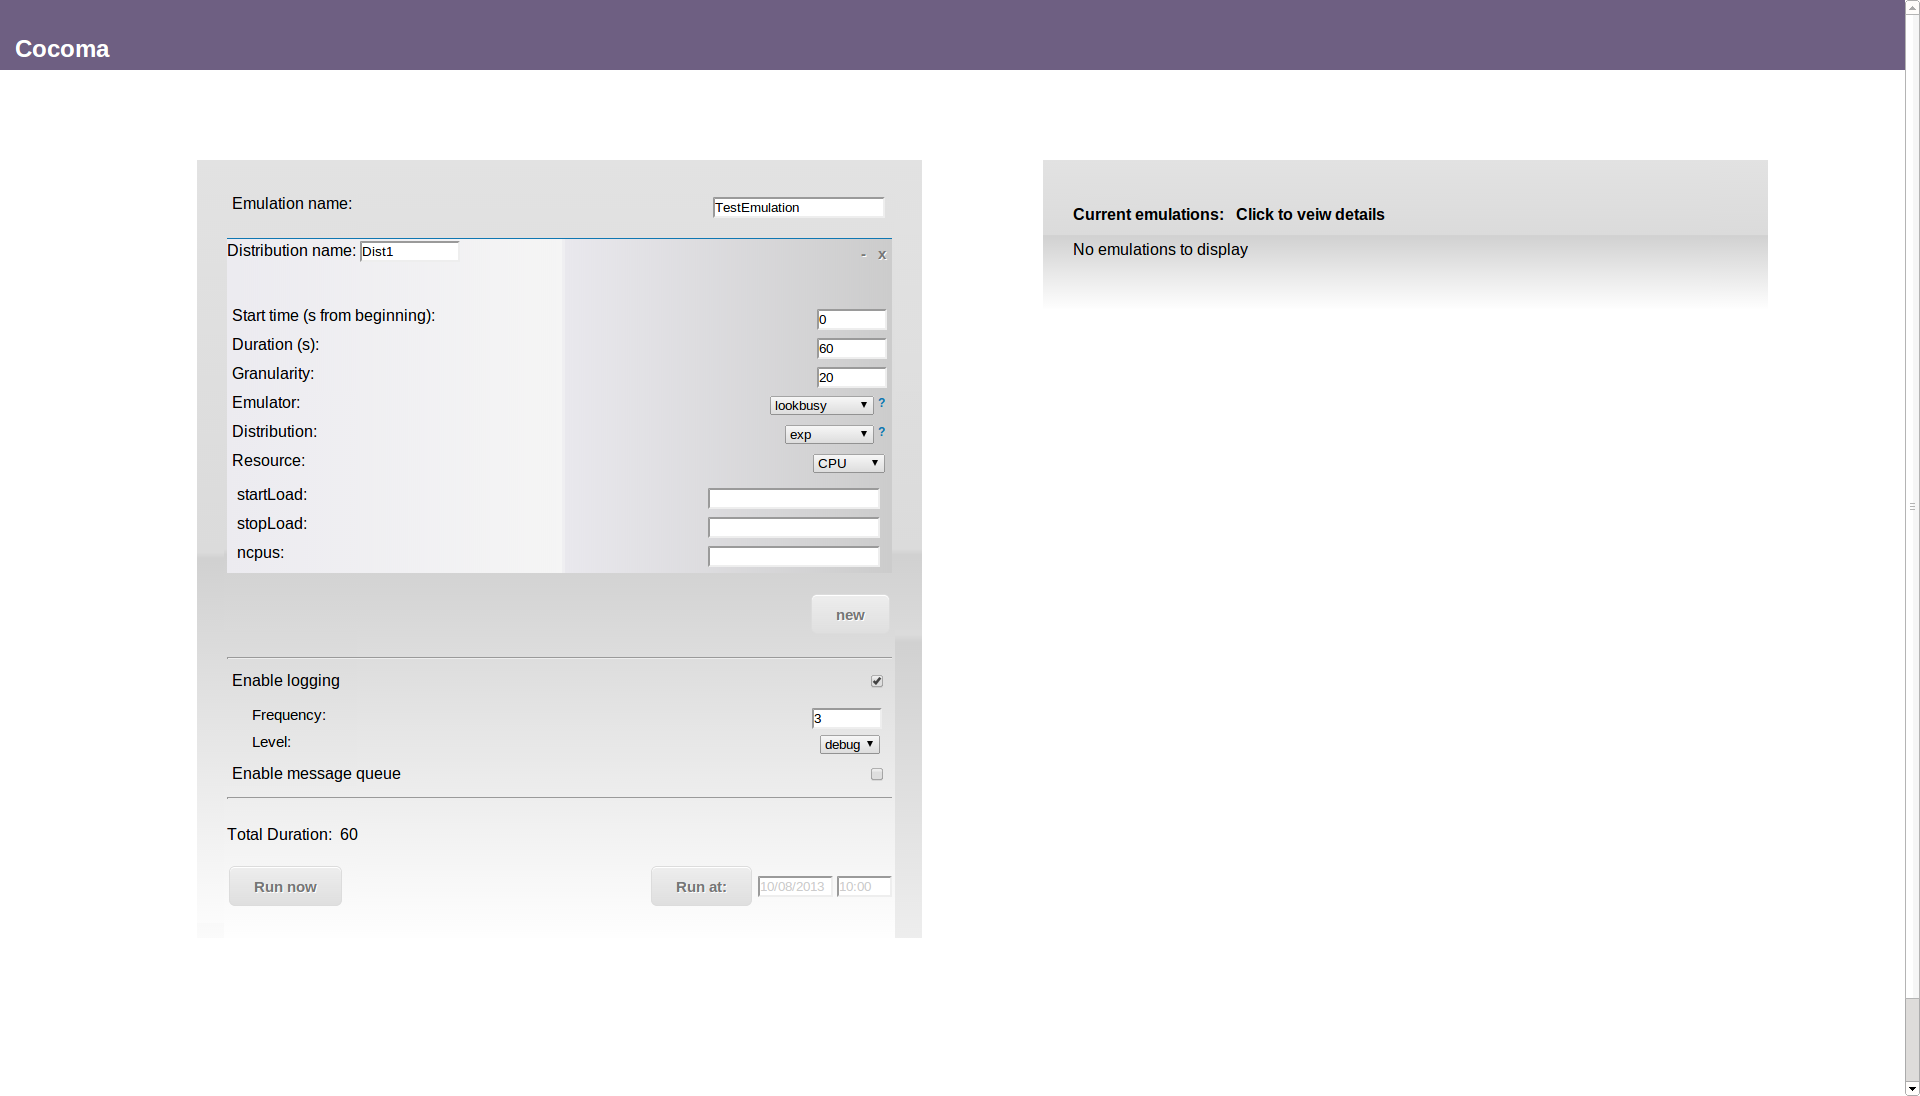
\includegraphics{Overall.png}}
\caption{COCOMA webUI}\end{figure}


\subsubsection{Creating an emulation}
\label{COCOMA/07_webUI:creating-an-emulation}
Each emulation requires a name and at least one distribution, although as many distributions as required can be added. Each distribution requires a name and all required fields to be filled, this data will vary as per the emulation, distribution or resource selected. Distribution windows can be minimized for overall readability or removed entirely (not added to the emulation) by clicking the `x' in the top right corner:
\begin{figure}[htbp]
\centering
\capstart

\scalebox{0.750000}{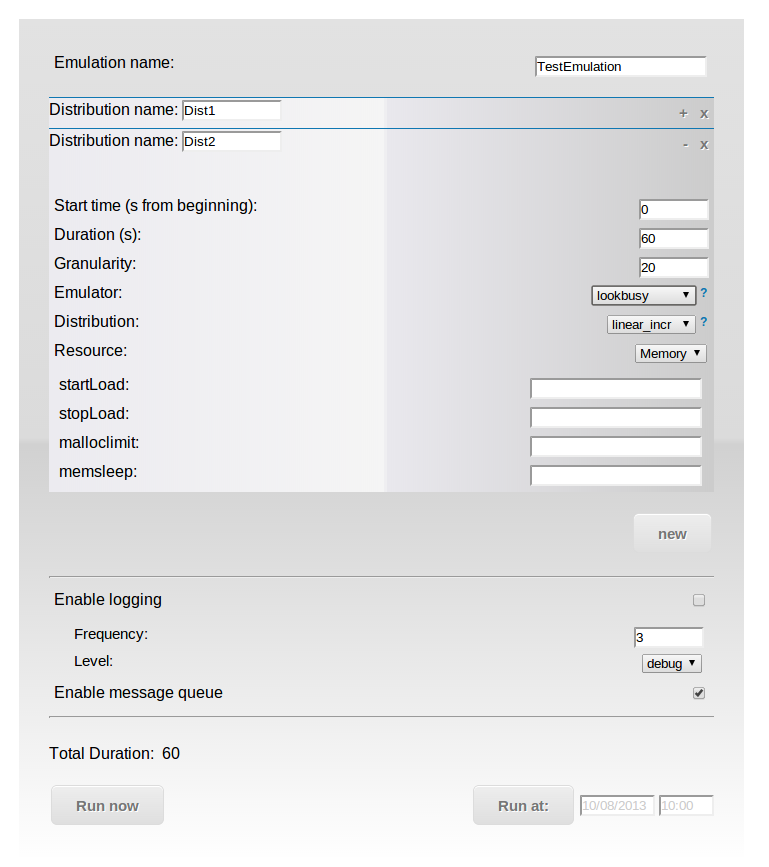
\includegraphics{MultiDist.png}}
\caption{Multi-distribution interface}\end{figure}


\subsubsection{Distribution Parameters}
\label{COCOMA/07_webUI:distribution-parameters}
\emph{Start time} determines how long (in seconds) after the overall emulation has begun, this particular distribution will begin. \emph{Duration} is how long the distribution will last for. \emph{Granularity} refers to the number of the steps taken from \emph{startLoad} through to \emph{stopLoad} over the course of the distributions run. For example a 60 second duration CPU stressing distribution with a granularity of 10 will move from \emph{startLoad} to \emph{stopLoad} in steps of 6 seconds. More information on the emulator or distribution currently selected and the specific parameters they require can be viewed by hovering over the blue question mark beside it:
\begin{figure}[htbp]
\centering
\capstart

\scalebox{0.900000}{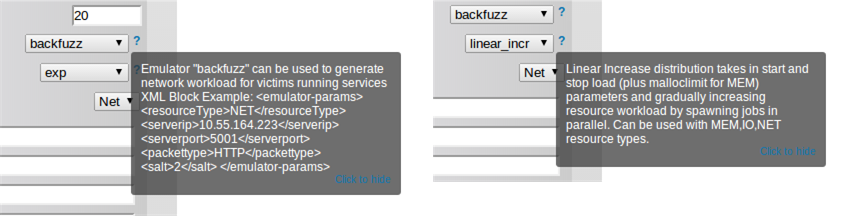
\includegraphics{ui_popup.png}}
\caption{Help pop-ups}\end{figure}


\subsubsection{Logging and Message Queue}
\label{COCOMA/07_webUI:logging-and-message-queue}
After the distributions have been created and specified, there is an option to enable or disable logging. Enabling logging give 2 more options, the \emph{frequency} in seconds and the \emph{level}, which dictates the amount of output the logs will contain. Below this is the option to enable or disable the message queue followed by various parameters allowing for it's setup
\begin{figure}[htbp]
\centering
\capstart

\scalebox{0.800000}{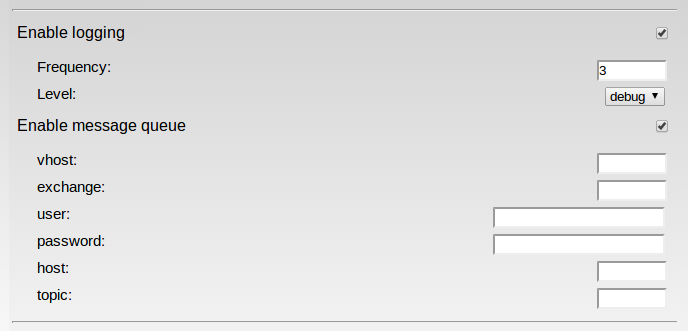
\includegraphics{logsandMQ.png}}
\caption{Logging and EMQ settings}\end{figure}


\subsubsection{Running the emulation}
\label{COCOMA/07_webUI:running-the-emulation}
Once all the parameters are set there are two options; run the emulation right away by clicking the \emph{Run now} button, or schedule the emulation to begin running at a set time in the future by clicking the \emph{Run at} button:
\begin{figure}[htbp]
\centering
\capstart

\scalebox{0.900000}{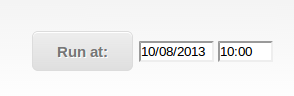
\includegraphics{runAt.png}}
\caption{Set time for emulation}\end{figure}


\subsubsection{Working with existing emulations}
\label{COCOMA/07_webUI:working-with-existing-emulations}
Any existing emulations in your system will be listed on the right hand side of the screen. The UI also displays the total number of runs, how many of those failed and the current state of the emulation (\emph{active} or \emph{inactive}). Hovering over the emulation name will display the information on that emulation in a popup and by clicking on it the emulation data
can be loaded into the creation screen on the left where its parameters can be edited or simply run again right away. Clicking the small download icon to the right of each emulation will prompt the download of a zip file to your system. This zip file contains the .xml used to create the emulation as well as .csv files with the system logs and the logs for that specific emulation.
\begin{figure}[htbp]
\centering
\capstart

\scalebox{0.900000}{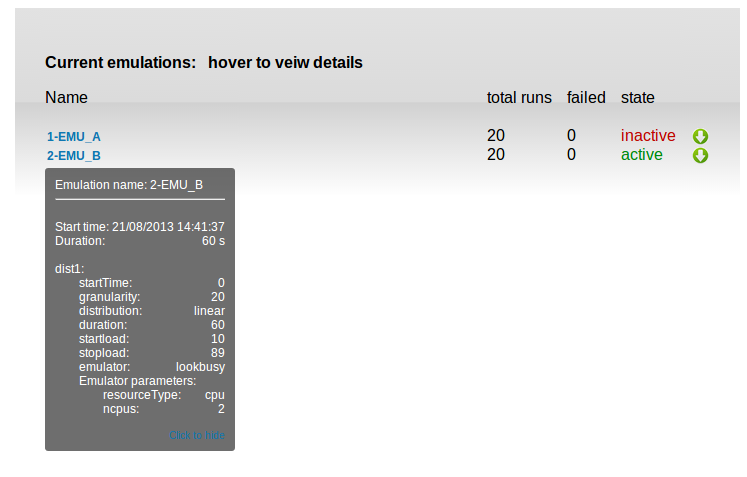
\includegraphics{emuDisplay.png}}
\caption{Emulations interface}\end{figure}


\subsection{XML Examples}
\label{COCOMA/05_examples::doc}\label{COCOMA/05_examples:xml-examples}
This section provides XML payload examples for creating different emulations over various resources.


\subsubsection{CPU}
\label{COCOMA/05_examples:cpu}
Emulation XML for CPU contention:

\begin{Verbatim}[commandchars=\\\{\},numbers=left,firstnumber=1,stepnumber=1]
\PYG{n+nt}{\PYGZlt{}emulation}\PYG{n+nt}{\PYGZgt{}}
  \PYG{n+nt}{\PYGZlt{}emuname}\PYG{n+nt}{\PYGZgt{}}CPU\PYGZus{}EMU\PYG{n+nt}{\PYGZlt{}/emuname\PYGZgt{}}
  \PYG{n+nt}{\PYGZlt{}emuType}\PYG{n+nt}{\PYGZgt{}}Mix\PYG{n+nt}{\PYGZlt{}/emuType\PYGZgt{}}
  \PYG{n+nt}{\PYGZlt{}emuresourceType}\PYG{n+nt}{\PYGZgt{}}CPU\PYG{n+nt}{\PYGZlt{}/emuresourceType\PYGZgt{}}
  \PYG{c}{\PYGZlt{}!\PYGZhy{}\PYGZhy{}}\PYG{c}{date format: 2014}\PYG{c}{\PYGZhy{}}\PYG{c}{10}\PYG{c}{\PYGZhy{}}\PYG{c}{10T10:10:10 }\PYG{c}{\PYGZhy{}\PYGZhy{}\PYGZgt{}}
  \PYG{n+nt}{\PYGZlt{}emustartTime}\PYG{n+nt}{\PYGZgt{}}now\PYG{n+nt}{\PYGZlt{}/emustartTime\PYGZgt{}}
  \PYG{c}{\PYGZlt{}!\PYGZhy{}\PYGZhy{}}\PYG{c}{duration in seconds }\PYG{c}{\PYGZhy{}\PYGZhy{}\PYGZgt{}}
  \PYG{n+nt}{\PYGZlt{}emustopTime}\PYG{n+nt}{\PYGZgt{}}120\PYG{n+nt}{\PYGZlt{}/emustopTime\PYGZgt{}}

  \PYG{n+nt}{\PYGZlt{}distributions}\PYG{n+nt}{\PYGZgt{}}
   \PYG{n+nt}{\PYGZlt{}name}\PYG{n+nt}{\PYGZgt{}}CPU\PYGZus{}Distro\PYG{n+nt}{\PYGZlt{}/name\PYGZgt{}}
     \PYG{n+nt}{\PYGZlt{}startTime}\PYG{n+nt}{\PYGZgt{}}0\PYG{n+nt}{\PYGZlt{}/startTime\PYGZgt{}}
     \PYG{c}{\PYGZlt{}!\PYGZhy{}\PYGZhy{}}\PYG{c}{duration in seconds }\PYG{c}{\PYGZhy{}\PYGZhy{}\PYGZgt{}}
     \PYG{n+nt}{\PYGZlt{}duration}\PYG{n+nt}{\PYGZgt{}}120\PYG{n+nt}{\PYGZlt{}/duration\PYGZgt{}}
     \PYG{n+nt}{\PYGZlt{}granularity}\PYG{n+nt}{\PYGZgt{}}24\PYG{n+nt}{\PYGZlt{}/granularity\PYGZgt{}}
     \PYG{n+nt}{\PYGZlt{}distribution} \PYG{n+na}{href=}\PYG{l+s}{\PYGZdq{}/distributions/linear\PYGZdq{}} \PYG{n+na}{name=}\PYG{l+s}{\PYGZdq{}linear\PYGZdq{}} \PYG{n+nt}{/\PYGZgt{}}
     \PYG{c}{\PYGZlt{}!\PYGZhy{}\PYGZhy{}}\PYG{c}{cpu utilization distribution range}\PYG{c}{\PYGZhy{}\PYGZhy{}\PYGZgt{}}
      \PYG{n+nt}{\PYGZlt{}startLoad}\PYG{n+nt}{\PYGZgt{}}10\PYG{n+nt}{\PYGZlt{}/startLoad\PYGZgt{}}
      \PYG{n+nt}{\PYGZlt{}stopLoad}\PYG{n+nt}{\PYGZgt{}}95\PYG{n+nt}{\PYGZlt{}/stopLoad\PYGZgt{}}
      \PYG{n+nt}{\PYGZlt{}emulator} \PYG{n+na}{href=}\PYG{l+s}{\PYGZdq{}/emulators/lookbusy\PYGZdq{}} \PYG{n+na}{name=}\PYG{l+s}{\PYGZdq{}lookbusy\PYGZdq{}} \PYG{n+nt}{/\PYGZgt{}}

      \PYG{n+nt}{\PYGZlt{}emulator\PYGZhy{}params}\PYG{n+nt}{\PYGZgt{}}
        \PYG{n+nt}{\PYGZlt{}resourceType}\PYG{n+nt}{\PYGZgt{}}CPU\PYG{n+nt}{\PYGZlt{}/resourceType\PYGZgt{}}
       \PYG{c}{\PYGZlt{}!\PYGZhy{}\PYGZhy{}}\PYG{c}{Number of CPUs to keep busy (default: autodetected)}\PYG{c}{\PYGZhy{}\PYGZhy{}\PYGZgt{}}
       \PYG{n+nt}{\PYGZlt{}ncpus}\PYG{n+nt}{\PYGZgt{}}1\PYG{n+nt}{\PYGZlt{}/ncpus\PYGZgt{}}
      \PYG{n+nt}{\PYGZlt{}/emulator\PYGZhy{}params\PYGZgt{}}
  \PYG{n+nt}{\PYGZlt{}/distributions\PYGZgt{}}

  \PYG{n+nt}{\PYGZlt{}log}\PYG{n+nt}{\PYGZgt{}}
   \PYG{c}{\PYGZlt{}!\PYGZhy{}\PYGZhy{}}\PYG{c}{ Use value \PYGZdq{}1\PYGZdq{} to enable logging(by default logging is off)  }\PYG{c}{\PYGZhy{}\PYGZhy{}\PYGZgt{}}
   \PYG{n+nt}{\PYGZlt{}enable}\PYG{n+nt}{\PYGZgt{}}1\PYG{n+nt}{\PYGZlt{}/enable\PYGZgt{}}
   \PYG{c}{\PYGZlt{}!\PYGZhy{}\PYGZhy{}}\PYG{c}{ Use seconds for setting probe intervals(if logging is enabled default is 3sec)  }\PYG{c}{\PYGZhy{}\PYGZhy{}\PYGZgt{}}
   \PYG{n+nt}{\PYGZlt{}frequency}\PYG{n+nt}{\PYGZgt{}}1\PYG{n+nt}{\PYGZlt{}/frequency\PYGZgt{}}
   \PYG{n+nt}{\PYGZlt{}logLevel}\PYG{n+nt}{\PYGZgt{}}debug\PYG{n+nt}{\PYGZlt{}/logLevel\PYGZgt{}}
  \PYG{n+nt}{\PYGZlt{}/log\PYGZgt{}}

\PYG{n+nt}{\PYGZlt{}/emulation\PYGZgt{}}
\end{Verbatim}


\subsubsection{I/O}
\label{COCOMA/05_examples:i-o}
Emulation XML for I/O contention:

\begin{Verbatim}[commandchars=\\\{\},numbers=left,firstnumber=1,stepnumber=1]
\PYG{n+nt}{\PYGZlt{}emulation}\PYG{n+nt}{\PYGZgt{}}
  \PYG{n+nt}{\PYGZlt{}emuname}\PYG{n+nt}{\PYGZgt{}}IO\PYGZus{}EMU\PYG{n+nt}{\PYGZlt{}/emuname\PYGZgt{}}
  \PYG{n+nt}{\PYGZlt{}emuType}\PYG{n+nt}{\PYGZgt{}}Mix\PYG{n+nt}{\PYGZlt{}/emuType\PYGZgt{}}
  \PYG{n+nt}{\PYGZlt{}emuresourceType}\PYG{n+nt}{\PYGZgt{}}IO\PYG{n+nt}{\PYGZlt{}/emuresourceType\PYGZgt{}}
  \PYG{c}{\PYGZlt{}!\PYGZhy{}\PYGZhy{}}\PYG{c}{date format: 2014}\PYG{c}{\PYGZhy{}}\PYG{c}{10}\PYG{c}{\PYGZhy{}}\PYG{c}{10T10:10:10 }\PYG{c}{\PYGZhy{}\PYGZhy{}\PYGZgt{}}
  \PYG{n+nt}{\PYGZlt{}emustartTime}\PYG{n+nt}{\PYGZgt{}}now\PYG{n+nt}{\PYGZlt{}/emustartTime\PYGZgt{}}
  \PYG{c}{\PYGZlt{}!\PYGZhy{}\PYGZhy{}}\PYG{c}{duration in seconds }\PYG{c}{\PYGZhy{}\PYGZhy{}\PYGZgt{}}
  \PYG{n+nt}{\PYGZlt{}emustopTime}\PYG{n+nt}{\PYGZgt{}}60\PYG{n+nt}{\PYGZlt{}/emustopTime\PYGZgt{}}

  \PYG{n+nt}{\PYGZlt{}distributions}\PYG{n+nt}{\PYGZgt{}}

   \PYG{n+nt}{\PYGZlt{}name}\PYG{n+nt}{\PYGZgt{}}IO\PYGZus{}Distro\PYG{n+nt}{\PYGZlt{}/name\PYGZgt{}}
     \PYG{n+nt}{\PYGZlt{}startTime}\PYG{n+nt}{\PYGZgt{}}0\PYG{n+nt}{\PYGZlt{}/startTime\PYGZgt{}}
     \PYG{c}{\PYGZlt{}!\PYGZhy{}\PYGZhy{}}\PYG{c}{duration in seconds }\PYG{c}{\PYGZhy{}\PYGZhy{}\PYGZgt{}}
     \PYG{n+nt}{\PYGZlt{}duration}\PYG{n+nt}{\PYGZgt{}}60\PYG{n+nt}{\PYGZlt{}/duration\PYGZgt{}}
     \PYG{n+nt}{\PYGZlt{}granularity}\PYG{n+nt}{\PYGZgt{}}5\PYG{n+nt}{\PYGZlt{}/granularity\PYGZgt{}}
     \PYG{n+nt}{\PYGZlt{}distribution} \PYG{n+na}{href=}\PYG{l+s}{\PYGZdq{}/distributions/linear\PYGZus{}incr\PYGZdq{}} \PYG{n+na}{name=}\PYG{l+s}{\PYGZdq{}linear\PYGZus{}incr\PYGZdq{}} \PYG{n+nt}{/\PYGZgt{}}
     \PYG{n+nt}{\PYGZlt{}startLoad}\PYG{n+nt}{\PYGZgt{}}1\PYG{n+nt}{\PYGZlt{}/startLoad\PYGZgt{}}
     \PYG{n+nt}{\PYGZlt{}stopLoad}\PYG{n+nt}{\PYGZgt{}}10\PYG{n+nt}{\PYGZlt{}/stopLoad\PYGZgt{}}
     \PYG{n+nt}{\PYGZlt{}emulator} \PYG{n+na}{href=}\PYG{l+s}{\PYGZdq{}/emulators/stressapptest\PYGZdq{}} \PYG{n+na}{name=}\PYG{l+s}{\PYGZdq{}stressapptest\PYGZdq{}} \PYG{n+nt}{/\PYGZgt{}}

      \PYG{n+nt}{\PYGZlt{}emulator\PYGZhy{}params}\PYG{n+nt}{\PYGZgt{}}
        \PYG{n+nt}{\PYGZlt{}resourceType}\PYG{n+nt}{\PYGZgt{}}IO\PYG{n+nt}{\PYGZlt{}/resourceType\PYGZgt{}}
        \PYG{c}{\PYGZlt{}!\PYGZhy{}\PYGZhy{}}\PYG{c}{Size of mem in MB used}\PYG{c}{\PYGZhy{}\PYGZhy{}\PYGZgt{}}
        \PYG{n+nt}{\PYGZlt{}memsize}\PYG{n+nt}{\PYGZgt{}}1000\PYG{n+nt}{\PYGZlt{}/memsize\PYGZgt{}}
        \PYG{c}{\PYGZlt{}!\PYGZhy{}\PYGZhy{}}\PYG{c}{Number of threads}\PYG{c}{\PYGZhy{}\PYGZhy{}\PYGZgt{}}
        \PYG{n+nt}{\PYGZlt{}memThreads}\PYG{n+nt}{\PYGZgt{}}10\PYG{n+nt}{\PYGZlt{}/memThreads\PYGZgt{}}
      \PYG{n+nt}{\PYGZlt{}/emulator\PYGZhy{}params\PYGZgt{}}

  \PYG{n+nt}{\PYGZlt{}/distributions\PYGZgt{}}

  \PYG{n+nt}{\PYGZlt{}log}\PYG{n+nt}{\PYGZgt{}}
   \PYG{c}{\PYGZlt{}!\PYGZhy{}\PYGZhy{}}\PYG{c}{ Use value \PYGZdq{}1\PYGZdq{} to enable logging(by default logging is off)  }\PYG{c}{\PYGZhy{}\PYGZhy{}\PYGZgt{}}
   \PYG{n+nt}{\PYGZlt{}enable}\PYG{n+nt}{\PYGZgt{}}1\PYG{n+nt}{\PYGZlt{}/enable\PYGZgt{}}
   \PYG{c}{\PYGZlt{}!\PYGZhy{}\PYGZhy{}}\PYG{c}{ Use seconds for setting probe intervals(if logging is enabled default is 3sec)  }\PYG{c}{\PYGZhy{}\PYGZhy{}\PYGZgt{}}
   \PYG{n+nt}{\PYGZlt{}frequency}\PYG{n+nt}{\PYGZgt{}}3\PYG{n+nt}{\PYGZlt{}/frequency\PYGZgt{}}
   \PYG{n+nt}{\PYGZlt{}logLevel}\PYG{n+nt}{\PYGZgt{}}debug\PYG{n+nt}{\PYGZlt{}/logLevel\PYGZgt{}}
  \PYG{n+nt}{\PYGZlt{}/log\PYGZgt{}}

\PYG{n+nt}{\PYGZlt{}/emulation\PYGZgt{}}
\end{Verbatim}

In this example we use a different distribution called \emph{trapezoidal}:

\begin{Verbatim}[commandchars=\\\{\},numbers=left,firstnumber=1,stepnumber=1]
\PYG{n+nt}{\PYGZlt{}emulation}\PYG{n+nt}{\PYGZgt{}}
  \PYG{n+nt}{\PYGZlt{}emuname}\PYG{n+nt}{\PYGZgt{}}IO\PYGZus{}EMU\PYG{n+nt}{\PYGZlt{}/emuname\PYGZgt{}}
  \PYG{n+nt}{\PYGZlt{}emuType}\PYG{n+nt}{\PYGZgt{}}Mix\PYG{n+nt}{\PYGZlt{}/emuType\PYGZgt{}}
  \PYG{n+nt}{\PYGZlt{}emuresourceType}\PYG{n+nt}{\PYGZgt{}}IO\PYG{n+nt}{\PYGZlt{}/emuresourceType\PYGZgt{}}
  \PYG{c}{\PYGZlt{}!\PYGZhy{}\PYGZhy{}}\PYG{c}{date format: 2014}\PYG{c}{\PYGZhy{}}\PYG{c}{10}\PYG{c}{\PYGZhy{}}\PYG{c}{10T10:10:10 }\PYG{c}{\PYGZhy{}\PYGZhy{}\PYGZgt{}}
  \PYG{n+nt}{\PYGZlt{}emustartTime}\PYG{n+nt}{\PYGZgt{}}now\PYG{n+nt}{\PYGZlt{}/emustartTime\PYGZgt{}}
  \PYG{c}{\PYGZlt{}!\PYGZhy{}\PYGZhy{}}\PYG{c}{duration in seconds }\PYG{c}{\PYGZhy{}\PYGZhy{}\PYGZgt{}}
  \PYG{n+nt}{\PYGZlt{}emustopTime}\PYG{n+nt}{\PYGZgt{}}60\PYG{n+nt}{\PYGZlt{}/emustopTime\PYGZgt{}}

  \PYG{n+nt}{\PYGZlt{}distributions}\PYG{n+nt}{\PYGZgt{}}

   \PYG{n+nt}{\PYGZlt{}name}\PYG{n+nt}{\PYGZgt{}}IO\PYGZus{}Distro\PYG{n+nt}{\PYGZlt{}/name\PYGZgt{}}
     \PYG{n+nt}{\PYGZlt{}startTime}\PYG{n+nt}{\PYGZgt{}}0\PYG{n+nt}{\PYGZlt{}/startTime\PYGZgt{}}
     \PYG{c}{\PYGZlt{}!\PYGZhy{}\PYGZhy{}}\PYG{c}{duration in seconds }\PYG{c}{\PYGZhy{}\PYGZhy{}\PYGZgt{}}
     \PYG{n+nt}{\PYGZlt{}duration}\PYG{n+nt}{\PYGZgt{}}60\PYG{n+nt}{\PYGZlt{}/duration\PYGZgt{}}
     \PYG{n+nt}{\PYGZlt{}granularity}\PYG{n+nt}{\PYGZgt{}}5\PYG{n+nt}{\PYGZlt{}/granularity\PYGZgt{}}
     \PYG{n+nt}{\PYGZlt{}distribution} \PYG{n+na}{href=}\PYG{l+s}{\PYGZdq{}/distributions/trapezoidal\PYGZdq{}} \PYG{n+na}{name=}\PYG{l+s}{\PYGZdq{}trapezoidal\PYGZdq{}} \PYG{n+nt}{/\PYGZgt{}}
     \PYG{n+nt}{\PYGZlt{}startLoad}\PYG{n+nt}{\PYGZgt{}}1\PYG{n+nt}{\PYGZlt{}/startLoad\PYGZgt{}}
     \PYG{n+nt}{\PYGZlt{}stopLoad}\PYG{n+nt}{\PYGZgt{}}10\PYG{n+nt}{\PYGZlt{}/stopLoad\PYGZgt{}}
     \PYG{n+nt}{\PYGZlt{}emulator} \PYG{n+na}{href=}\PYG{l+s}{\PYGZdq{}/emulators/stressapptest\PYGZdq{}} \PYG{n+na}{name=}\PYG{l+s}{\PYGZdq{}stressapptest\PYGZdq{}} \PYG{n+nt}{/\PYGZgt{}}

      \PYG{n+nt}{\PYGZlt{}emulator\PYGZhy{}params}\PYG{n+nt}{\PYGZgt{}}
        \PYG{n+nt}{\PYGZlt{}resourceType}\PYG{n+nt}{\PYGZgt{}}IO\PYG{n+nt}{\PYGZlt{}/resourceType\PYGZgt{}}
        \PYG{c}{\PYGZlt{}!\PYGZhy{}\PYGZhy{}}\PYG{c}{Size of mem in MB used}\PYG{c}{\PYGZhy{}\PYGZhy{}\PYGZgt{}}
        \PYG{n+nt}{\PYGZlt{}memsize}\PYG{n+nt}{\PYGZgt{}}1000\PYG{n+nt}{\PYGZlt{}/memsize\PYGZgt{}}
        \PYG{c}{\PYGZlt{}!\PYGZhy{}\PYGZhy{}}\PYG{c}{Number of threads}\PYG{c}{\PYGZhy{}\PYGZhy{}\PYGZgt{}}
        \PYG{n+nt}{\PYGZlt{}memThreads}\PYG{n+nt}{\PYGZgt{}}10\PYG{n+nt}{\PYGZlt{}/memThreads\PYGZgt{}}
      \PYG{n+nt}{\PYGZlt{}/emulator\PYGZhy{}params\PYGZgt{}}

  \PYG{n+nt}{\PYGZlt{}/distributions\PYGZgt{}}

  \PYG{n+nt}{\PYGZlt{}log}\PYG{n+nt}{\PYGZgt{}}
   \PYG{c}{\PYGZlt{}!\PYGZhy{}\PYGZhy{}}\PYG{c}{ Use value \PYGZdq{}1\PYGZdq{} to enable logging(by default logging is off)  }\PYG{c}{\PYGZhy{}\PYGZhy{}\PYGZgt{}}
   \PYG{n+nt}{\PYGZlt{}enable}\PYG{n+nt}{\PYGZgt{}}1\PYG{n+nt}{\PYGZlt{}/enable\PYGZgt{}}
   \PYG{c}{\PYGZlt{}!\PYGZhy{}\PYGZhy{}}\PYG{c}{ Use seconds for setting probe intervals(if logging is enabled default is 3sec)  }\PYG{c}{\PYGZhy{}\PYGZhy{}\PYGZgt{}}
   \PYG{n+nt}{\PYGZlt{}frequency}\PYG{n+nt}{\PYGZgt{}}3\PYG{n+nt}{\PYGZlt{}/frequency\PYGZgt{}}
   \PYG{n+nt}{\PYGZlt{}logLevel}\PYG{n+nt}{\PYGZgt{}}debug\PYG{n+nt}{\PYGZlt{}/logLevel\PYGZgt{}}
  \PYG{n+nt}{\PYGZlt{}/log\PYGZgt{}}

\PYG{n+nt}{\PYGZlt{}/emulation\PYGZgt{}}
\end{Verbatim}


\subsubsection{Memory}
\label{COCOMA/05_examples:memory}
Emulation XML for memory contention:

\begin{Verbatim}[commandchars=\\\{\},numbers=left,firstnumber=1,stepnumber=1]
\PYG{n+nt}{\PYGZlt{}emulation}\PYG{n+nt}{\PYGZgt{}}
  \PYG{n+nt}{\PYGZlt{}emuname}\PYG{n+nt}{\PYGZgt{}}MEM\PYGZus{}EMU\PYG{n+nt}{\PYGZlt{}/emuname\PYGZgt{}}
  \PYG{n+nt}{\PYGZlt{}emuType}\PYG{n+nt}{\PYGZgt{}}Mix\PYG{n+nt}{\PYGZlt{}/emuType\PYGZgt{}}
  \PYG{n+nt}{\PYGZlt{}emuresourceType}\PYG{n+nt}{\PYGZgt{}}MEM\PYG{n+nt}{\PYGZlt{}/emuresourceType\PYGZgt{}}
  \PYG{c}{\PYGZlt{}!\PYGZhy{}\PYGZhy{}}\PYG{c}{date format: 2014}\PYG{c}{\PYGZhy{}}\PYG{c}{10}\PYG{c}{\PYGZhy{}}\PYG{c}{10T10:10:10 }\PYG{c}{\PYGZhy{}\PYGZhy{}\PYGZgt{}}
  \PYG{n+nt}{\PYGZlt{}emustartTime}\PYG{n+nt}{\PYGZgt{}}now\PYG{n+nt}{\PYGZlt{}/emustartTime\PYGZgt{}}
  \PYG{c}{\PYGZlt{}!\PYGZhy{}\PYGZhy{}}\PYG{c}{duration in seconds }\PYG{c}{\PYGZhy{}\PYGZhy{}\PYGZgt{}}
  \PYG{n+nt}{\PYGZlt{}emustopTime}\PYG{n+nt}{\PYGZgt{}}60\PYG{n+nt}{\PYGZlt{}/emustopTime\PYGZgt{}}

  \PYG{n+nt}{\PYGZlt{}distributions} \PYG{n+nt}{\PYGZgt{}}
     \PYG{n+nt}{\PYGZlt{}name}\PYG{n+nt}{\PYGZgt{}}MEM\PYGZus{}Distro\PYG{n+nt}{\PYGZlt{}/name\PYGZgt{}}
     \PYG{n+nt}{\PYGZlt{}startTime}\PYG{n+nt}{\PYGZgt{}}0\PYG{n+nt}{\PYGZlt{}/startTime\PYGZgt{}}
     \PYG{c}{\PYGZlt{}!\PYGZhy{}\PYGZhy{}}\PYG{c}{duration in seconds }\PYG{c}{\PYGZhy{}\PYGZhy{}\PYGZgt{}}
     \PYG{n+nt}{\PYGZlt{}duration}\PYG{n+nt}{\PYGZgt{}}60\PYG{n+nt}{\PYGZlt{}/duration\PYGZgt{}}
     \PYG{n+nt}{\PYGZlt{}granularity}\PYG{n+nt}{\PYGZgt{}}5\PYG{n+nt}{\PYGZlt{}/granularity\PYGZgt{}}
     \PYG{n+nt}{\PYGZlt{}distribution} \PYG{n+na}{href=}\PYG{l+s}{\PYGZdq{}/distributions/linear\PYGZus{}incr\PYGZdq{}} \PYG{n+na}{name=}\PYG{l+s}{\PYGZdq{}linear\PYGZus{}incr\PYGZdq{}} \PYG{n+nt}{/\PYGZgt{}}
     \PYG{c}{\PYGZlt{}!\PYGZhy{}\PYGZhy{}}\PYG{c}{Memory usage (Megabytes) }\PYG{c}{\PYGZhy{}\PYGZhy{}\PYGZgt{}}
     \PYG{n+nt}{\PYGZlt{}startLoad}\PYG{n+nt}{\PYGZgt{}}100\PYG{n+nt}{\PYGZlt{}/startLoad\PYGZgt{}}
     \PYG{n+nt}{\PYGZlt{}stopLoad}\PYG{n+nt}{\PYGZgt{}}1000\PYG{n+nt}{\PYGZlt{}/stopLoad\PYGZgt{}}
     \PYG{n+nt}{\PYGZlt{}malloclimit}\PYG{n+nt}{\PYGZgt{}}4095\PYG{n+nt}{\PYGZlt{}/malloclimit\PYGZgt{}}
     \PYG{n+nt}{\PYGZlt{}emulator} \PYG{n+na}{href=}\PYG{l+s}{\PYGZdq{}/emulators/stressapptest\PYGZdq{}} \PYG{n+na}{name=}\PYG{l+s}{\PYGZdq{}stressapptest\PYGZdq{}} \PYG{n+nt}{/\PYGZgt{}}
     \PYG{n+nt}{\PYGZlt{}emulator\PYGZhy{}params}\PYG{n+nt}{\PYGZgt{}}
         \PYG{n+nt}{\PYGZlt{}resourceType}\PYG{n+nt}{\PYGZgt{}}MEM\PYG{n+nt}{\PYGZlt{}/resourceType\PYGZgt{}}
         \PYG{n+nt}{\PYGZlt{}memThreads}\PYG{n+nt}{\PYGZgt{}}0\PYG{n+nt}{\PYGZlt{}/memThreads\PYGZgt{}}
     \PYG{n+nt}{\PYGZlt{}/emulator\PYGZhy{}params\PYGZgt{}}
  \PYG{n+nt}{\PYGZlt{}/distributions\PYGZgt{}}

  \PYG{n+nt}{\PYGZlt{}log}\PYG{n+nt}{\PYGZgt{}}
   \PYG{c}{\PYGZlt{}!\PYGZhy{}\PYGZhy{}}\PYG{c}{ Use value \PYGZdq{}1\PYGZdq{} to enable logging(by default logging is off)  }\PYG{c}{\PYGZhy{}\PYGZhy{}\PYGZgt{}}
   \PYG{n+nt}{\PYGZlt{}enable}\PYG{n+nt}{\PYGZgt{}}1\PYG{n+nt}{\PYGZlt{}/enable\PYGZgt{}}
   \PYG{c}{\PYGZlt{}!\PYGZhy{}\PYGZhy{}}\PYG{c}{ Use seconds for setting probe intervals(if logging is enabled default is 3sec)  }\PYG{c}{\PYGZhy{}\PYGZhy{}\PYGZgt{}}
   \PYG{n+nt}{\PYGZlt{}frequency}\PYG{n+nt}{\PYGZgt{}}3\PYG{n+nt}{\PYGZlt{}/frequency\PYGZgt{}}
   \PYG{n+nt}{\PYGZlt{}logLevel}\PYG{n+nt}{\PYGZgt{}}debug\PYG{n+nt}{\PYGZlt{}/logLevel\PYGZgt{}}
  \PYG{n+nt}{\PYGZlt{}/log\PYGZgt{}}

\PYG{n+nt}{\PYGZlt{}/emulation\PYGZgt{}}
\end{Verbatim}

Example for memory emulation using \emph{trapezoidal} distribution:

\begin{Verbatim}[commandchars=\\\{\},numbers=left,firstnumber=1,stepnumber=1]
\PYG{n+nt}{\PYGZlt{}emulation}\PYG{n+nt}{\PYGZgt{}}
  \PYG{n+nt}{\PYGZlt{}emuname}\PYG{n+nt}{\PYGZgt{}}MEM\PYGZus{}EMU\PYG{n+nt}{\PYGZlt{}/emuname\PYGZgt{}}
  \PYG{n+nt}{\PYGZlt{}emuType}\PYG{n+nt}{\PYGZgt{}}Mix\PYG{n+nt}{\PYGZlt{}/emuType\PYGZgt{}}
  \PYG{n+nt}{\PYGZlt{}emuresourceType}\PYG{n+nt}{\PYGZgt{}}MEM\PYG{n+nt}{\PYGZlt{}/emuresourceType\PYGZgt{}}
  \PYG{c}{\PYGZlt{}!\PYGZhy{}\PYGZhy{}}\PYG{c}{date format: 2014}\PYG{c}{\PYGZhy{}}\PYG{c}{10}\PYG{c}{\PYGZhy{}}\PYG{c}{10T10:10:10 }\PYG{c}{\PYGZhy{}\PYGZhy{}\PYGZgt{}}
  \PYG{n+nt}{\PYGZlt{}emustartTime}\PYG{n+nt}{\PYGZgt{}}now\PYG{n+nt}{\PYGZlt{}/emustartTime\PYGZgt{}}
  \PYG{c}{\PYGZlt{}!\PYGZhy{}\PYGZhy{}}\PYG{c}{duration in seconds }\PYG{c}{\PYGZhy{}\PYGZhy{}\PYGZgt{}}
  \PYG{n+nt}{\PYGZlt{}emustopTime}\PYG{n+nt}{\PYGZgt{}}60\PYG{n+nt}{\PYGZlt{}/emustopTime\PYGZgt{}}

  \PYG{n+nt}{\PYGZlt{}distributions} \PYG{n+nt}{\PYGZgt{}}
     \PYG{n+nt}{\PYGZlt{}name}\PYG{n+nt}{\PYGZgt{}}MEM\PYGZus{}Distro\PYG{n+nt}{\PYGZlt{}/name\PYGZgt{}}
     \PYG{n+nt}{\PYGZlt{}startTime}\PYG{n+nt}{\PYGZgt{}}0\PYG{n+nt}{\PYGZlt{}/startTime\PYGZgt{}}
     \PYG{c}{\PYGZlt{}!\PYGZhy{}\PYGZhy{}}\PYG{c}{duration in seconds }\PYG{c}{\PYGZhy{}\PYGZhy{}\PYGZgt{}}
     \PYG{n+nt}{\PYGZlt{}duration}\PYG{n+nt}{\PYGZgt{}}60\PYG{n+nt}{\PYGZlt{}/duration\PYGZgt{}}
     \PYG{n+nt}{\PYGZlt{}granularity}\PYG{n+nt}{\PYGZgt{}}5\PYG{n+nt}{\PYGZlt{}/granularity\PYGZgt{}}
     \PYG{n+nt}{\PYGZlt{}distribution} \PYG{n+na}{href=}\PYG{l+s}{\PYGZdq{}/distributions/trapezoidal\PYGZdq{}} \PYG{n+na}{name=}\PYG{l+s}{\PYGZdq{}trapezoidal\PYGZdq{}} \PYG{n+nt}{/\PYGZgt{}}
     \PYG{c}{\PYGZlt{}!\PYGZhy{}\PYGZhy{}}\PYG{c}{Megabytes for memory }\PYG{c}{\PYGZhy{}\PYGZhy{}\PYGZgt{}}
     \PYG{n+nt}{\PYGZlt{}startLoad}\PYG{n+nt}{\PYGZgt{}}100\PYG{n+nt}{\PYGZlt{}/startLoad\PYGZgt{}}
     \PYG{n+nt}{\PYGZlt{}stopLoad}\PYG{n+nt}{\PYGZgt{}}1000\PYG{n+nt}{\PYGZlt{}/stopLoad\PYGZgt{}}
     \PYG{n+nt}{\PYGZlt{}malloclimit}\PYG{n+nt}{\PYGZgt{}}4095\PYG{n+nt}{\PYGZlt{}/malloclimit\PYGZgt{}}
     \PYG{n+nt}{\PYGZlt{}emulator} \PYG{n+na}{href=}\PYG{l+s}{\PYGZdq{}/emulators/stressapptest\PYGZdq{}} \PYG{n+na}{name=}\PYG{l+s}{\PYGZdq{}stressapptest\PYGZdq{}} \PYG{n+nt}{/\PYGZgt{}}
     \PYG{n+nt}{\PYGZlt{}emulator\PYGZhy{}params}\PYG{n+nt}{\PYGZgt{}}
         \PYG{n+nt}{\PYGZlt{}resourceType}\PYG{n+nt}{\PYGZgt{}}MEM\PYG{n+nt}{\PYGZlt{}/resourceType\PYGZgt{}}
         \PYG{n+nt}{\PYGZlt{}memThreads}\PYG{n+nt}{\PYGZgt{}}0\PYG{n+nt}{\PYGZlt{}/memThreads\PYGZgt{}}
     \PYG{n+nt}{\PYGZlt{}/emulator\PYGZhy{}params\PYGZgt{}}
  \PYG{n+nt}{\PYGZlt{}/distributions\PYGZgt{}}

  \PYG{n+nt}{\PYGZlt{}log}\PYG{n+nt}{\PYGZgt{}}
   \PYG{c}{\PYGZlt{}!\PYGZhy{}\PYGZhy{}}\PYG{c}{ Use value \PYGZdq{}1\PYGZdq{} to enable logging(by default logging is off)  }\PYG{c}{\PYGZhy{}\PYGZhy{}\PYGZgt{}}
   \PYG{n+nt}{\PYGZlt{}enable}\PYG{n+nt}{\PYGZgt{}}0\PYG{n+nt}{\PYGZlt{}/enable\PYGZgt{}}
   \PYG{c}{\PYGZlt{}!\PYGZhy{}\PYGZhy{}}\PYG{c}{ Use seconds for setting probe intervals(if logging is enabled default is 3sec)  }\PYG{c}{\PYGZhy{}\PYGZhy{}\PYGZgt{}}
   \PYG{n+nt}{\PYGZlt{}frequency}\PYG{n+nt}{\PYGZgt{}}3\PYG{n+nt}{\PYGZlt{}/frequency\PYGZgt{}}
   \PYG{n+nt}{\PYGZlt{}logLevel}\PYG{n+nt}{\PYGZgt{}}debug\PYG{n+nt}{\PYGZlt{}/logLevel\PYGZgt{}}
  \PYG{n+nt}{\PYGZlt{}/log\PYGZgt{}}

\PYG{n+nt}{\PYGZlt{}/emulation\PYGZgt{}}
\end{Verbatim}


\subsubsection{Network}
\label{COCOMA/05_examples:network}
The newtork emulation needs two COCOMA VM's, one that acts as a client and the other as a server. Normally those two VMs are placed in different nodes. The SuT should be composed of at least two VMs placed on the same two nodes of COCOMA. The emulation XML for network contention looks like:

\begin{Verbatim}[commandchars=\\\{\},numbers=left,firstnumber=1,stepnumber=1]
\PYG{n+nt}{\PYGZlt{}emulation}\PYG{n+nt}{\PYGZgt{}}
  \PYG{n+nt}{\PYGZlt{}emuname}\PYG{n+nt}{\PYGZgt{}}NET\PYGZus{}emu\PYG{n+nt}{\PYGZlt{}/emuname\PYGZgt{}}
  \PYG{n+nt}{\PYGZlt{}emuType}\PYG{n+nt}{\PYGZgt{}}Mix\PYG{n+nt}{\PYGZlt{}/emuType\PYGZgt{}}
  \PYG{n+nt}{\PYGZlt{}emuresourceType}\PYG{n+nt}{\PYGZgt{}}NET\PYG{n+nt}{\PYGZlt{}/emuresourceType\PYGZgt{}}
  \PYG{c}{\PYGZlt{}!\PYGZhy{}\PYGZhy{}}\PYG{c}{2014}\PYG{c}{\PYGZhy{}}\PYG{c}{02}\PYG{c}{\PYGZhy{}}\PYG{c}{02T10:10:10}\PYG{c}{\PYGZhy{}\PYGZhy{}\PYGZgt{}}
  \PYG{n+nt}{\PYGZlt{}emustartTime}\PYG{n+nt}{\PYGZgt{}}now\PYG{n+nt}{\PYGZlt{}/emustartTime\PYGZgt{}}
  \PYG{c}{\PYGZlt{}!\PYGZhy{}\PYGZhy{}}\PYG{c}{duration in seconds }\PYG{c}{\PYGZhy{}\PYGZhy{}\PYGZgt{}}
  \PYG{n+nt}{\PYGZlt{}emustopTime}\PYG{n+nt}{\PYGZgt{}}155\PYG{n+nt}{\PYGZlt{}/emustopTime\PYGZgt{}}

  \PYG{n+nt}{\PYGZlt{}distributions}\PYG{n+nt}{\PYGZgt{}}
     \PYG{n+nt}{\PYGZlt{}name}\PYG{n+nt}{\PYGZgt{}}NET\PYGZus{}distro\PYG{n+nt}{\PYGZlt{}/name\PYGZgt{}}
     \PYG{n+nt}{\PYGZlt{}startTime}\PYG{n+nt}{\PYGZgt{}}0\PYG{n+nt}{\PYGZlt{}/startTime\PYGZgt{}}
     \PYG{c}{\PYGZlt{}!\PYGZhy{}\PYGZhy{}}\PYG{c}{duration in seconds }\PYG{c}{\PYGZhy{}\PYGZhy{}\PYGZgt{}}
     \PYG{n+nt}{\PYGZlt{}duration}\PYG{n+nt}{\PYGZgt{}}150\PYG{n+nt}{\PYGZlt{}/duration\PYGZgt{}}
     \PYG{n+nt}{\PYGZlt{}granularity}\PYG{n+nt}{\PYGZgt{}}10\PYG{n+nt}{\PYGZlt{}/granularity\PYGZgt{}}
     \PYG{n+nt}{\PYGZlt{}distribution} \PYG{n+na}{href=}\PYG{l+s}{\PYGZdq{}/distributions/linear\PYGZus{}incr\PYGZdq{}} \PYG{n+na}{name=}\PYG{l+s}{\PYGZdq{}linear\PYGZus{}incr\PYGZdq{}} \PYG{n+nt}{/\PYGZgt{}}
     \PYG{c}{\PYGZlt{}!\PYGZhy{}\PYGZhy{}}\PYG{c}{set target bandwidth to bits per sec}\PYG{c}{\PYGZhy{}\PYGZhy{}\PYGZgt{}}
     \PYG{n+nt}{\PYGZlt{}startLoad}\PYG{n+nt}{\PYGZgt{}}100\PYG{n+nt}{\PYGZlt{}/startLoad\PYGZgt{}}
     \PYG{n+nt}{\PYGZlt{}stopLoad}\PYG{n+nt}{\PYGZgt{}}1000\PYG{n+nt}{\PYGZlt{}/stopLoad\PYGZgt{}}
     \PYG{n+nt}{\PYGZlt{}emulator} \PYG{n+na}{href=}\PYG{l+s}{\PYGZdq{}/emulators/iperf\PYGZdq{}} \PYG{n+na}{name=}\PYG{l+s}{\PYGZdq{}iperf\PYGZdq{}} \PYG{n+nt}{/\PYGZgt{}}
     \PYG{n+nt}{\PYGZlt{}emulator\PYGZhy{}params}\PYG{n+nt}{\PYGZgt{}}
        \PYG{n+nt}{\PYGZlt{}resourceType}\PYG{n+nt}{\PYGZgt{}}NET\PYG{n+nt}{\PYGZlt{}/resourceType\PYGZgt{}}
        \PYG{n+nt}{\PYGZlt{}serverip}\PYG{n+nt}{\PYGZgt{}}172.18.254.234\PYG{n+nt}{\PYGZlt{}/serverip\PYGZgt{}}
        \PYG{c}{\PYGZlt{}!\PYGZhy{}\PYGZhy{}}\PYG{c}{Leave \PYGZdq{}0\PYGZdq{} for default 5001 port }\PYG{c}{\PYGZhy{}\PYGZhy{}\PYGZgt{}}
        \PYG{n+nt}{\PYGZlt{}serverport}\PYG{n+nt}{\PYGZgt{}}5001\PYG{n+nt}{\PYGZlt{}/serverport\PYGZgt{}}
        \PYG{n+nt}{\PYGZlt{}clientip}\PYG{n+nt}{\PYGZgt{}}172.18.254.236\PYG{n+nt}{\PYGZlt{}/clientip\PYGZgt{}}
        \PYG{n+nt}{\PYGZlt{}clientport}\PYG{n+nt}{\PYGZgt{}}5001\PYG{n+nt}{\PYGZlt{}/clientport\PYGZgt{}}
        \PYG{n+nt}{\PYGZlt{}packettype}\PYG{n+nt}{\PYGZgt{}}UDP\PYG{n+nt}{\PYGZlt{}/packettype\PYGZgt{}}
        \PYG{n+nt}{\PYGZlt{}/emulator\PYGZhy{}params\PYGZgt{}}
  \PYG{n+nt}{\PYGZlt{}/distributions\PYGZgt{}}

  \PYG{n+nt}{\PYGZlt{}log}\PYG{n+nt}{\PYGZgt{}}
   \PYG{c}{\PYGZlt{}!\PYGZhy{}\PYGZhy{}}\PYG{c}{ Use value \PYGZdq{}1\PYGZdq{} to enable logging(by default logging is off)  }\PYG{c}{\PYGZhy{}\PYGZhy{}\PYGZgt{}}
   \PYG{n+nt}{\PYGZlt{}enable}\PYG{n+nt}{\PYGZgt{}}0\PYG{n+nt}{\PYGZlt{}/enable\PYGZgt{}}
   \PYG{c}{\PYGZlt{}!\PYGZhy{}\PYGZhy{}}\PYG{c}{ Use seconds for setting probe intervals(if logging is enabled default is 3sec)  }\PYG{c}{\PYGZhy{}\PYGZhy{}\PYGZgt{}}
   \PYG{n+nt}{\PYGZlt{}frequency}\PYG{n+nt}{\PYGZgt{}}3\PYG{n+nt}{\PYGZlt{}/frequency\PYGZgt{}}
  \PYG{n+nt}{\PYGZlt{}/log\PYGZgt{}}

\PYG{n+nt}{\PYGZlt{}/emulation\PYGZgt{}}
\end{Verbatim}

In the following example a different emulator named \emph{backfuzz} will be used with its proprietary distribution \emph{fuzz}. This combination is used to simulate malicious network activity by sending a series of random requests and data to the specified server

\begin{Verbatim}[commandchars=\\\{\},numbers=left,firstnumber=1,stepnumber=1]
\PYG{n+nt}{\PYGZlt{}emulation}\PYG{n+nt}{\PYGZgt{}}
 \PYG{n+nt}{\PYGZlt{}emuname}\PYG{n+nt}{\PYGZgt{}}MAL\PYGZus{}EMU\PYG{n+nt}{\PYGZlt{}/emuname\PYGZgt{}}
 \PYG{n+nt}{\PYGZlt{}emuType}\PYG{n+nt}{\PYGZgt{}}NET\PYG{n+nt}{\PYGZlt{}/emuType\PYGZgt{}}
 \PYG{n+nt}{\PYGZlt{}emuresourceType}\PYG{n+nt}{\PYGZgt{}}NET\PYG{n+nt}{\PYGZlt{}/emuresourceType\PYGZgt{}}
 \PYG{c}{\PYGZlt{}!\PYGZhy{}\PYGZhy{}}\PYG{c}{date format: 2014}\PYG{c}{\PYGZhy{}}\PYG{c}{10}\PYG{c}{\PYGZhy{}}\PYG{c}{10T10:10:10 }\PYG{c}{\PYGZhy{}\PYGZhy{}\PYGZgt{}}
 \PYG{n+nt}{\PYGZlt{}emustartTime}\PYG{n+nt}{\PYGZgt{}}now\PYG{n+nt}{\PYGZlt{}/emustartTime\PYGZgt{}}
 \PYG{c}{\PYGZlt{}!\PYGZhy{}\PYGZhy{}}\PYG{c}{duration in seconds }\PYG{c}{\PYGZhy{}\PYGZhy{}\PYGZgt{}}
 \PYG{n+nt}{\PYGZlt{}emustopTime}\PYG{n+nt}{\PYGZgt{}}120\PYG{n+nt}{\PYGZlt{}/emustopTime\PYGZgt{}}

 \PYG{n+nt}{\PYGZlt{}distributions}\PYG{n+nt}{\PYGZgt{}}
    \PYG{n+nt}{\PYGZlt{}name}\PYG{n+nt}{\PYGZgt{}}MAL\PYGZus{}Distro1\PYG{n+nt}{\PYGZlt{}/name\PYGZgt{}}
    \PYG{n+nt}{\PYGZlt{}startTime}\PYG{n+nt}{\PYGZgt{}}0\PYG{n+nt}{\PYGZlt{}/startTime\PYGZgt{}}
    \PYG{n+nt}{\PYGZlt{}duration}\PYG{n+nt}{\PYGZgt{}}120\PYG{n+nt}{\PYGZlt{}/duration\PYGZgt{}}
    \PYG{n+nt}{\PYGZlt{}distribution} \PYG{n+na}{href=}\PYG{l+s}{\PYGZdq{}/distributions/fuzz\PYGZdq{}} \PYG{n+na}{name=}\PYG{l+s}{\PYGZdq{}fuzz\PYGZdq{}} \PYG{n+nt}{/\PYGZgt{}}
    \PYG{n+nt}{\PYGZlt{}startLoad}\PYG{n+nt}{\PYGZgt{}}100\PYG{n+nt}{\PYGZlt{}/startLoad\PYGZgt{}}
    \PYG{n+nt}{\PYGZlt{}emulator} \PYG{n+na}{href=}\PYG{l+s}{\PYGZdq{}/emulators/backfuzz\PYGZdq{}} \PYG{n+na}{name=}\PYG{l+s}{\PYGZdq{}backfuzz\PYGZdq{}} \PYG{n+nt}{/\PYGZgt{}}
    \PYG{n+nt}{\PYGZlt{}emulator\PYGZhy{}params}\PYG{n+nt}{\PYGZgt{}}
        \PYG{n+nt}{\PYGZlt{}resourceType}\PYG{n+nt}{\PYGZgt{}}NET\PYG{n+nt}{\PYGZlt{}/resourceType\PYGZgt{}}
        \PYG{c}{\PYGZlt{}!\PYGZhy{}\PYGZhy{}}\PYG{c}{ Difference between MIN and MAX fuzz values }\PYG{c}{\PYGZhy{}\PYGZhy{}\PYGZgt{}}
        \PYG{n+nt}{\PYGZlt{}fuzzRange}\PYG{n+nt}{\PYGZgt{}}900\PYG{n+nt}{\PYGZlt{}/fuzzRange\PYGZgt{}}
        \PYG{c}{\PYGZlt{}!\PYGZhy{}\PYGZhy{}}\PYG{c}{ IP and port of server to fuzz }\PYG{c}{\PYGZhy{}\PYGZhy{}\PYGZgt{}}
        \PYG{n+nt}{\PYGZlt{}serverip}\PYG{n+nt}{\PYGZgt{}}10.55.168.238\PYG{n+nt}{\PYGZlt{}/serverip\PYGZgt{}}
        \PYG{n+nt}{\PYGZlt{}serverport}\PYG{n+nt}{\PYGZgt{}}51889\PYG{n+nt}{\PYGZlt{}/serverport\PYGZgt{}}
        \PYG{c}{\PYGZlt{}!\PYGZhy{}\PYGZhy{}}\PYG{c}{ Type of packet to use for fuzzing }\PYG{c}{\PYGZhy{}\PYGZhy{}\PYGZgt{}}
        \PYG{n+nt}{\PYGZlt{}packettype}\PYG{n+nt}{\PYGZgt{}}HTTP\PYG{n+nt}{\PYGZlt{}/packettype\PYGZgt{}}
        \PYG{c}{\PYGZlt{}!\PYGZhy{}\PYGZhy{}}\PYG{c}{ Time to pause on each fuzz value in s (leave as 0 for default of 0.8s) }\PYG{c}{\PYGZhy{}\PYGZhy{}\PYGZgt{}}
        \PYG{n+nt}{\PYGZlt{}timedelay}\PYG{n+nt}{\PYGZgt{}}1\PYG{n+nt}{\PYGZlt{}/timedelay\PYGZgt{}}
        \PYG{c}{\PYGZlt{}!\PYGZhy{}\PYGZhy{}}\PYG{c}{ Value to increment by }\PYG{c}{\PYGZhy{}\PYGZhy{}\PYGZgt{}}
        \PYG{n+nt}{\PYGZlt{}salt}\PYG{n+nt}{\PYGZgt{}}50\PYG{n+nt}{\PYGZlt{}/salt\PYGZgt{}}
    \PYG{n+nt}{\PYGZlt{}/emulator\PYGZhy{}params\PYGZgt{}}
 \PYG{n+nt}{\PYGZlt{}/distributions\PYGZgt{}}

 \PYG{n+nt}{\PYGZlt{}log}\PYG{n+nt}{\PYGZgt{}}
  \PYG{c}{\PYGZlt{}!\PYGZhy{}\PYGZhy{}}\PYG{c}{ Use value \PYGZdq{}1\PYGZdq{} to enable logging(by default logging is off)  }\PYG{c}{\PYGZhy{}\PYGZhy{}\PYGZgt{}}
  \PYG{n+nt}{\PYGZlt{}enable}\PYG{n+nt}{\PYGZgt{}}0\PYG{n+nt}{\PYGZlt{}/enable\PYGZgt{}}
  \PYG{c}{\PYGZlt{}!\PYGZhy{}\PYGZhy{}}\PYG{c}{ Use seconds for setting probe intervals(if logging is enabled default is 3sec)  }\PYG{c}{\PYGZhy{}\PYGZhy{}\PYGZgt{}}
  \PYG{n+nt}{\PYGZlt{}frequency}\PYG{n+nt}{\PYGZgt{}}3\PYG{n+nt}{\PYGZlt{}/frequency\PYGZgt{}}
  \PYG{n+nt}{\PYGZlt{}logLevel}\PYG{n+nt}{\PYGZgt{}}debug\PYG{n+nt}{\PYGZlt{}/logLevel\PYGZgt{}}
 \PYG{n+nt}{\PYGZlt{}/log\PYGZgt{}}

\PYG{n+nt}{\PYGZlt{}/emulation\PYGZgt{}}
\end{Verbatim}


\subsubsection{Multiple distributions emulation}
\label{COCOMA/05_examples:multiple-distributions-emulation}
An important feature of COCOMA is the ability to combine multiple distributions within the same emulation. This allows to specify contention properties for multiple resources or create different patterns for the same resource. Distributions can overlap, meaning two distributions can run at the same time frame. If distributions for the same resource overlap and they exceed the available resources, the runs might crash.
\begin{itemize}
\item {} 
CPU and Memory example

\end{itemize}

\begin{Verbatim}[commandchars=\\\{\},numbers=left,firstnumber=1,stepnumber=1]
 \PYG{n+nt}{\PYGZlt{}emulation}\PYG{n+nt}{\PYGZgt{}}
     \PYG{n+nt}{\PYGZlt{}emuname}\PYG{n+nt}{\PYGZgt{}}CPU\PYGZus{}and\PYGZus{}Mem\PYG{n+nt}{\PYGZlt{}/emuname\PYGZgt{}}
     \PYG{n+nt}{\PYGZlt{}emutype}\PYG{n+nt}{\PYGZgt{}}Mix\PYG{n+nt}{\PYGZlt{}/emutype\PYGZgt{}}
     \PYG{n+nt}{\PYGZlt{}emuresourceType}\PYG{n+nt}{\PYGZgt{}}MIX\PYG{n+nt}{\PYGZlt{}/emuresourceType\PYGZgt{}}
     \PYG{n+nt}{\PYGZlt{}emustartTime}\PYG{n+nt}{\PYGZgt{}}now\PYG{n+nt}{\PYGZlt{}/emustartTime\PYGZgt{}}
     \PYG{c}{\PYGZlt{}!\PYGZhy{}\PYGZhy{}}\PYG{c}{duration in seconds }\PYG{c}{\PYGZhy{}\PYGZhy{}\PYGZgt{}}
     \PYG{n+nt}{\PYGZlt{}emustopTime}\PYG{n+nt}{\PYGZgt{}}80\PYG{n+nt}{\PYGZlt{}/emustopTime\PYGZgt{}}

     \PYG{n+nt}{\PYGZlt{}distributions}\PYG{n+nt}{\PYGZgt{}}
        \PYG{n+nt}{\PYGZlt{}name}\PYG{n+nt}{\PYGZgt{}}CPU\PYGZus{}distro\PYG{n+nt}{\PYGZlt{}/name\PYGZgt{}}
        \PYG{n+nt}{\PYGZlt{}startTime}\PYG{n+nt}{\PYGZgt{}}0\PYG{n+nt}{\PYGZlt{}/startTime\PYGZgt{}}
        \PYG{c}{\PYGZlt{}!\PYGZhy{}\PYGZhy{}}\PYG{c}{duration in seconds }\PYG{c}{\PYGZhy{}\PYGZhy{}\PYGZgt{}}
        \PYG{n+nt}{\PYGZlt{}duration}\PYG{n+nt}{\PYGZgt{}}60\PYG{n+nt}{\PYGZlt{}/duration\PYGZgt{}}
        \PYG{n+nt}{\PYGZlt{}granularity}\PYG{n+nt}{\PYGZgt{}}1\PYG{n+nt}{\PYGZlt{}/granularity\PYGZgt{}}
        \PYG{n+nt}{\PYGZlt{}distribution} \PYG{n+na}{href=}\PYG{l+s}{\PYGZdq{}/distributions/linear\PYGZdq{}} \PYG{n+na}{name=}\PYG{l+s}{\PYGZdq{}linear\PYGZdq{}} \PYG{n+nt}{/\PYGZgt{}}
        \PYG{c}{\PYGZlt{}!\PYGZhy{}\PYGZhy{}}\PYG{c}{cpu utilization distribution range}\PYG{c}{\PYGZhy{}\PYGZhy{}\PYGZgt{}}
        \PYG{n+nt}{\PYGZlt{}startLoad}\PYG{n+nt}{\PYGZgt{}}10\PYG{n+nt}{\PYGZlt{}/startLoad\PYGZgt{}}
        \PYG{n+nt}{\PYGZlt{}stopLoad}\PYG{n+nt}{\PYGZgt{}}95\PYG{n+nt}{\PYGZlt{}/stopLoad\PYGZgt{}}
        \PYG{n+nt}{\PYGZlt{}emulator} \PYG{n+na}{href=}\PYG{l+s}{\PYGZdq{}/emulators/lookbusy\PYGZdq{}} \PYG{n+na}{name=}\PYG{l+s}{\PYGZdq{}lookbusy\PYGZdq{}} \PYG{n+nt}{/\PYGZgt{}}
        \PYG{n+nt}{\PYGZlt{}emulator\PYGZhy{}params}\PYG{n+nt}{\PYGZgt{}}
             \PYG{n+nt}{\PYGZlt{}resourceType}\PYG{n+nt}{\PYGZgt{}}CPU\PYG{n+nt}{\PYGZlt{}/resourceType\PYGZgt{}}
             \PYG{c}{\PYGZlt{}!\PYGZhy{}\PYGZhy{}}\PYG{c}{Number of CPUs to keep busy (default: autodetected)}\PYG{c}{\PYGZhy{}\PYGZhy{}\PYGZgt{}}
             \PYG{n+nt}{\PYGZlt{}ncpus}\PYG{n+nt}{\PYGZgt{}}0\PYG{n+nt}{\PYGZlt{}/ncpus\PYGZgt{}}
        \PYG{n+nt}{\PYGZlt{}/emulator\PYGZhy{}params\PYGZgt{}}
     \PYG{n+nt}{\PYGZlt{}/distributions\PYGZgt{}}

     \PYG{n+nt}{\PYGZlt{}distributions}\PYG{n+nt}{\PYGZgt{}}
         \PYG{n+nt}{\PYGZlt{}name}\PYG{n+nt}{\PYGZgt{}}MEM\PYGZus{}Distro\PYG{n+nt}{\PYGZlt{}/name\PYGZgt{}}
         \PYG{n+nt}{\PYGZlt{}startTime}\PYG{n+nt}{\PYGZgt{}}20\PYG{n+nt}{\PYGZlt{}/startTime\PYGZgt{}}
         \PYG{c}{\PYGZlt{}!\PYGZhy{}\PYGZhy{}}\PYG{c}{duration in seconds }\PYG{c}{\PYGZhy{}\PYGZhy{}\PYGZgt{}}
         \PYG{n+nt}{\PYGZlt{}duration}\PYG{n+nt}{\PYGZgt{}}60\PYG{n+nt}{\PYGZlt{}/duration\PYGZgt{}}
         \PYG{n+nt}{\PYGZlt{}granularity}\PYG{n+nt}{\PYGZgt{}}5\PYG{n+nt}{\PYGZlt{}/granularity\PYGZgt{}}
         \PYG{n+nt}{\PYGZlt{}distribution} \PYG{n+na}{href=}\PYG{l+s}{\PYGZdq{}/distributions/linear\PYGZus{}incr\PYGZdq{}} \PYG{n+na}{name=}\PYG{l+s}{\PYGZdq{}linear\PYGZus{}incr\PYGZdq{}} \PYG{n+nt}{/\PYGZgt{}}
         \PYG{c}{\PYGZlt{}!\PYGZhy{}\PYGZhy{}}\PYG{c}{Megabytes for memory }\PYG{c}{\PYGZhy{}\PYGZhy{}\PYGZgt{}}
         \PYG{n+nt}{\PYGZlt{}startLoad}\PYG{n+nt}{\PYGZgt{}}100\PYG{n+nt}{\PYGZlt{}/startLoad\PYGZgt{}}
         \PYG{n+nt}{\PYGZlt{}stopLoad}\PYG{n+nt}{\PYGZgt{}}1000\PYG{n+nt}{\PYGZlt{}/stopLoad\PYGZgt{}}
         \PYG{n+nt}{\PYGZlt{}malloclimit}\PYG{n+nt}{\PYGZgt{}}4095\PYG{n+nt}{\PYGZlt{}/malloclimit\PYGZgt{}}
         \PYG{n+nt}{\PYGZlt{}emulator} \PYG{n+na}{href=}\PYG{l+s}{\PYGZdq{}/emulators/stressapptest\PYGZdq{}} \PYG{n+na}{name=}\PYG{l+s}{\PYGZdq{}stressapptest\PYGZdq{}} \PYG{n+nt}{/\PYGZgt{}}
         \PYG{n+nt}{\PYGZlt{}emulator\PYGZhy{}params}\PYG{n+nt}{\PYGZgt{}}
           \PYG{n+nt}{\PYGZlt{}resourceType}\PYG{n+nt}{\PYGZgt{}}MEM\PYG{n+nt}{\PYGZlt{}/resourceType\PYGZgt{}}
           \PYG{n+nt}{\PYGZlt{}memThreads}\PYG{n+nt}{\PYGZgt{}}0\PYG{n+nt}{\PYGZlt{}/memThreads\PYGZgt{}}
         \PYG{n+nt}{\PYGZlt{}/emulator\PYGZhy{}params\PYGZgt{}}
     \PYG{n+nt}{\PYGZlt{}/distributions\PYGZgt{}}

     \PYG{n+nt}{\PYGZlt{}log}\PYG{n+nt}{\PYGZgt{}}
        \PYG{c}{\PYGZlt{}!\PYGZhy{}\PYGZhy{}}\PYG{c}{ Use value \PYGZdq{}1\PYGZdq{} to enable logging(by default logging is off)  }\PYG{c}{\PYGZhy{}\PYGZhy{}\PYGZgt{}}
        \PYG{n+nt}{\PYGZlt{}enable}\PYG{n+nt}{\PYGZgt{}}1\PYG{n+nt}{\PYGZlt{}/enable\PYGZgt{}}
        \PYG{c}{\PYGZlt{}!\PYGZhy{}\PYGZhy{}}\PYG{c}{ Use seconds for setting probe intervals(if logging is enabled default is 3sec)  }\PYG{c}{\PYGZhy{}\PYGZhy{}\PYGZgt{}}
        \PYG{n+nt}{\PYGZlt{}frequency}\PYG{n+nt}{\PYGZgt{}}3\PYG{n+nt}{\PYGZlt{}/frequency\PYGZgt{}}
     \PYG{n+nt}{\PYGZlt{}/log\PYGZgt{}}
 \PYG{n+nt}{\PYGZlt{}/emulation\PYGZgt{}}
\end{Verbatim}
\begin{itemize}
\item {} 
CPU, MEM and IO example

\end{itemize}

\begin{Verbatim}[commandchars=\\\{\},numbers=left,firstnumber=1,stepnumber=1]
 \PYG{n+nt}{\PYGZlt{}emulation}\PYG{n+nt}{\PYGZgt{}}
     \PYG{n+nt}{\PYGZlt{}emuname}\PYG{n+nt}{\PYGZgt{}}CPU\PYGZus{}and\PYGZus{}Mem\PYG{n+nt}{\PYGZlt{}/emuname\PYGZgt{}}
     \PYG{n+nt}{\PYGZlt{}emutype}\PYG{n+nt}{\PYGZgt{}}Mix\PYG{n+nt}{\PYGZlt{}/emutype\PYGZgt{}}
     \PYG{n+nt}{\PYGZlt{}emuresourceType}\PYG{n+nt}{\PYGZgt{}}MIX\PYG{n+nt}{\PYGZlt{}/emuresourceType\PYGZgt{}}
     \PYG{n+nt}{\PYGZlt{}emustartTime}\PYG{n+nt}{\PYGZgt{}}now\PYG{n+nt}{\PYGZlt{}/emustartTime\PYGZgt{}}
     \PYG{c}{\PYGZlt{}!\PYGZhy{}\PYGZhy{}}\PYG{c}{duration in seconds }\PYG{c}{\PYGZhy{}\PYGZhy{}\PYGZgt{}}
     \PYG{n+nt}{\PYGZlt{}emustopTime}\PYG{n+nt}{\PYGZgt{}}80\PYG{n+nt}{\PYGZlt{}/emustopTime\PYGZgt{}}

     \PYG{n+nt}{\PYGZlt{}distributions}\PYG{n+nt}{\PYGZgt{}}
         \PYG{n+nt}{\PYGZlt{}name}\PYG{n+nt}{\PYGZgt{}}CPU\PYGZus{}distro\PYG{n+nt}{\PYGZlt{}/name\PYGZgt{}}
         \PYG{n+nt}{\PYGZlt{}startTime}\PYG{n+nt}{\PYGZgt{}}0\PYG{n+nt}{\PYGZlt{}/startTime\PYGZgt{}}
         \PYG{c}{\PYGZlt{}!\PYGZhy{}\PYGZhy{}}\PYG{c}{duration in seconds }\PYG{c}{\PYGZhy{}\PYGZhy{}\PYGZgt{}}
         \PYG{n+nt}{\PYGZlt{}duration}\PYG{n+nt}{\PYGZgt{}}60\PYG{n+nt}{\PYGZlt{}/duration\PYGZgt{}}
         \PYG{n+nt}{\PYGZlt{}granularity}\PYG{n+nt}{\PYGZgt{}}1\PYG{n+nt}{\PYGZlt{}/granularity\PYGZgt{}}
         \PYG{n+nt}{\PYGZlt{}distribution} \PYG{n+na}{href=}\PYG{l+s}{\PYGZdq{}/distributions/linear\PYGZdq{}} \PYG{n+na}{name=}\PYG{l+s}{\PYGZdq{}linear\PYGZdq{}} \PYG{n+nt}{/\PYGZgt{}}
         \PYG{c}{\PYGZlt{}!\PYGZhy{}\PYGZhy{}}\PYG{c}{cpu utilization distribution range}\PYG{c}{\PYGZhy{}\PYGZhy{}\PYGZgt{}}
         \PYG{n+nt}{\PYGZlt{}startLoad}\PYG{n+nt}{\PYGZgt{}}10\PYG{n+nt}{\PYGZlt{}/startLoad\PYGZgt{}}
         \PYG{n+nt}{\PYGZlt{}stopLoad}\PYG{n+nt}{\PYGZgt{}}95\PYG{n+nt}{\PYGZlt{}/stopLoad\PYGZgt{}}
         \PYG{n+nt}{\PYGZlt{}emulator} \PYG{n+na}{href=}\PYG{l+s}{\PYGZdq{}/emulators/lookbusy\PYGZdq{}} \PYG{n+na}{name=}\PYG{l+s}{\PYGZdq{}lookbusy\PYGZdq{}} \PYG{n+nt}{/\PYGZgt{}}
         \PYG{n+nt}{\PYGZlt{}emulator\PYGZhy{}params}\PYG{n+nt}{\PYGZgt{}}
              \PYG{n+nt}{\PYGZlt{}resourceType}\PYG{n+nt}{\PYGZgt{}}CPU\PYG{n+nt}{\PYGZlt{}/resourceType\PYGZgt{}}
              \PYG{c}{\PYGZlt{}!\PYGZhy{}\PYGZhy{}}\PYG{c}{Number of CPUs to keep busy (default: autodetected)}\PYG{c}{\PYGZhy{}\PYGZhy{}\PYGZgt{}}
              \PYG{n+nt}{\PYGZlt{}ncpus}\PYG{n+nt}{\PYGZgt{}}0\PYG{n+nt}{\PYGZlt{}/ncpus\PYGZgt{}}
         \PYG{n+nt}{\PYGZlt{}/emulator\PYGZhy{}params\PYGZgt{}}
      \PYG{n+nt}{\PYGZlt{}/distributions\PYGZgt{}}

      \PYG{n+nt}{\PYGZlt{}distributions} \PYG{n+nt}{\PYGZgt{}}
         \PYG{n+nt}{\PYGZlt{}name}\PYG{n+nt}{\PYGZgt{}}MEM\PYGZus{}Distro\PYG{n+nt}{\PYGZlt{}/name\PYGZgt{}}
         \PYG{n+nt}{\PYGZlt{}startTime}\PYG{n+nt}{\PYGZgt{}}20\PYG{n+nt}{\PYGZlt{}/startTime\PYGZgt{}}
         \PYG{c}{\PYGZlt{}!\PYGZhy{}\PYGZhy{}}\PYG{c}{duration in seconds }\PYG{c}{\PYGZhy{}\PYGZhy{}\PYGZgt{}}
         \PYG{n+nt}{\PYGZlt{}duration}\PYG{n+nt}{\PYGZgt{}}60\PYG{n+nt}{\PYGZlt{}/duration\PYGZgt{}}
         \PYG{n+nt}{\PYGZlt{}granularity}\PYG{n+nt}{\PYGZgt{}}5\PYG{n+nt}{\PYGZlt{}/granularity\PYGZgt{}}
         \PYG{n+nt}{\PYGZlt{}distribution} \PYG{n+na}{href=}\PYG{l+s}{\PYGZdq{}/distributions/linear\PYGZus{}incr\PYGZdq{}} \PYG{n+na}{name=}\PYG{l+s}{\PYGZdq{}linear\PYGZus{}incr\PYGZdq{}} \PYG{n+nt}{/\PYGZgt{}}
         \PYG{c}{\PYGZlt{}!\PYGZhy{}\PYGZhy{}}\PYG{c}{Megabytes for memory }\PYG{c}{\PYGZhy{}\PYGZhy{}\PYGZgt{}}
         \PYG{n+nt}{\PYGZlt{}startLoad}\PYG{n+nt}{\PYGZgt{}}100\PYG{n+nt}{\PYGZlt{}/startLoad\PYGZgt{}}
         \PYG{n+nt}{\PYGZlt{}stopLoad}\PYG{n+nt}{\PYGZgt{}}1000\PYG{n+nt}{\PYGZlt{}/stopLoad\PYGZgt{}}
         \PYG{n+nt}{\PYGZlt{}malloclimit}\PYG{n+nt}{\PYGZgt{}}4095\PYG{n+nt}{\PYGZlt{}/malloclimit\PYGZgt{}}
         \PYG{n+nt}{\PYGZlt{}emulator} \PYG{n+na}{href=}\PYG{l+s}{\PYGZdq{}/emulators/stressapptest\PYGZdq{}} \PYG{n+na}{name=}\PYG{l+s}{\PYGZdq{}stressapptest\PYGZdq{}} \PYG{n+nt}{/\PYGZgt{}}
         \PYG{n+nt}{\PYGZlt{}emulator\PYGZhy{}params}\PYG{n+nt}{\PYGZgt{}}
            \PYG{n+nt}{\PYGZlt{}resourceType}\PYG{n+nt}{\PYGZgt{}}MEM\PYG{n+nt}{\PYGZlt{}/resourceType\PYGZgt{}}
            \PYG{n+nt}{\PYGZlt{}memThreads}\PYG{n+nt}{\PYGZgt{}}0\PYG{n+nt}{\PYGZlt{}/memThreads\PYGZgt{}}
         \PYG{n+nt}{\PYGZlt{}/emulator\PYGZhy{}params\PYGZgt{}}
      \PYG{n+nt}{\PYGZlt{}/distributions\PYGZgt{}}

     \PYG{n+nt}{\PYGZlt{}distributions}\PYG{n+nt}{\PYGZgt{}}
         \PYG{n+nt}{\PYGZlt{}name}\PYG{n+nt}{\PYGZgt{}}IO\PYGZus{}Distro\PYG{n+nt}{\PYGZlt{}/name\PYGZgt{}}
         \PYG{n+nt}{\PYGZlt{}startTime}\PYG{n+nt}{\PYGZgt{}}0\PYG{n+nt}{\PYGZlt{}/startTime\PYGZgt{}}
         \PYG{c}{\PYGZlt{}!\PYGZhy{}\PYGZhy{}}\PYG{c}{duration in seconds }\PYG{c}{\PYGZhy{}\PYGZhy{}\PYGZgt{}}
         \PYG{n+nt}{\PYGZlt{}duration}\PYG{n+nt}{\PYGZgt{}}60\PYG{n+nt}{\PYGZlt{}/duration\PYGZgt{}}
         \PYG{n+nt}{\PYGZlt{}granularity}\PYG{n+nt}{\PYGZgt{}}5\PYG{n+nt}{\PYGZlt{}/granularity\PYGZgt{}}
         \PYG{n+nt}{\PYGZlt{}distribution} \PYG{n+na}{href=}\PYG{l+s}{\PYGZdq{}/distributions/linear\PYGZus{}incr\PYGZdq{}} \PYG{n+na}{name=}\PYG{l+s}{\PYGZdq{}linear\PYGZus{}incr\PYGZdq{}} \PYG{n+nt}{/\PYGZgt{}}
         \PYG{n+nt}{\PYGZlt{}startLoad}\PYG{n+nt}{\PYGZgt{}}1\PYG{n+nt}{\PYGZlt{}/startLoad\PYGZgt{}}
         \PYG{n+nt}{\PYGZlt{}stopLoad}\PYG{n+nt}{\PYGZgt{}}10\PYG{n+nt}{\PYGZlt{}/stopLoad\PYGZgt{}}
         \PYG{n+nt}{\PYGZlt{}emulator} \PYG{n+na}{href=}\PYG{l+s}{\PYGZdq{}/emulators/lookbusy\PYGZdq{}} \PYG{n+na}{name=}\PYG{l+s}{\PYGZdq{}lookbusy\PYGZdq{}} \PYG{n+nt}{/\PYGZgt{}}
         \PYG{n+nt}{\PYGZlt{}emulator\PYGZhy{}params}\PYG{n+nt}{\PYGZgt{}}
             \PYG{n+nt}{\PYGZlt{}resourceType}\PYG{n+nt}{\PYGZgt{}}IO\PYG{n+nt}{\PYGZlt{}/resourceType\PYGZgt{}}
             \PYG{c}{\PYGZlt{}!\PYGZhy{}\PYGZhy{}}\PYG{c}{Size of blocks to use for I/O, in MB}\PYG{c}{\PYGZhy{}\PYGZhy{}\PYGZgt{}}
             \PYG{n+nt}{\PYGZlt{}ioBlockSize}\PYG{n+nt}{\PYGZgt{}}10\PYG{n+nt}{\PYGZlt{}/ioBlockSize\PYGZgt{}}
             \PYG{c}{\PYGZlt{}!\PYGZhy{}\PYGZhy{}}\PYG{c}{Time to sleep between iterations, in msec}\PYG{c}{\PYGZhy{}\PYGZhy{}\PYGZgt{}}
            \PYG{n+nt}{\PYGZlt{}ioSleep}\PYG{n+nt}{\PYGZgt{}}100\PYG{n+nt}{\PYGZlt{}/ioSleep\PYGZgt{}}
        \PYG{n+nt}{\PYGZlt{}/emulator\PYGZhy{}params\PYGZgt{}}
    \PYG{n+nt}{\PYGZlt{}/distributions\PYGZgt{}}

    \PYG{n+nt}{\PYGZlt{}log}\PYG{n+nt}{\PYGZgt{}}
       \PYG{c}{\PYGZlt{}!\PYGZhy{}\PYGZhy{}}\PYG{c}{ Use value \PYGZdq{}1\PYGZdq{} to enable logging(by default logging is off)  }\PYG{c}{\PYGZhy{}\PYGZhy{}\PYGZgt{}}
       \PYG{n+nt}{\PYGZlt{}enable}\PYG{n+nt}{\PYGZgt{}}1\PYG{n+nt}{\PYGZlt{}/enable\PYGZgt{}}
       \PYG{c}{\PYGZlt{}!\PYGZhy{}\PYGZhy{}}\PYG{c}{ Use seconds for setting probe intervals(if logging is enabled default is 3sec)  }\PYG{c}{\PYGZhy{}\PYGZhy{}\PYGZgt{}}
       \PYG{n+nt}{\PYGZlt{}frequency}\PYG{n+nt}{\PYGZgt{}}3\PYG{n+nt}{\PYGZlt{}/frequency\PYGZgt{}}
    \PYG{n+nt}{\PYGZlt{}/log\PYGZgt{}}
 \PYG{n+nt}{\PYGZlt{}/emulation\PYGZgt{}}
\end{Verbatim}


\subsubsection{Known Issues}
\label{COCOMA/05_examples:known-issues}
The interaction of the various emulators used in COCOMA can cause unexpected issues. Some of these issues are listed below (This is \emph{not} an exhaustive list, and will be updated as new issues are discovered)
\begin{itemize}
\item {} 
Stressapptest uses \textasciitilde{}100\% CPU, regardless of what resource it is being ran on.

\item {} 
If a Linear increase distribution is run on memory using stressapptest at the same time as Iperf is being used to load the Network, then the Network resource may not reach its target load. This problem is usually encountered when the memory usage reaches over \textasciitilde{}80\% (as shown in the graph below)

\end{itemize}
\begin{figure}[htbp]
\centering

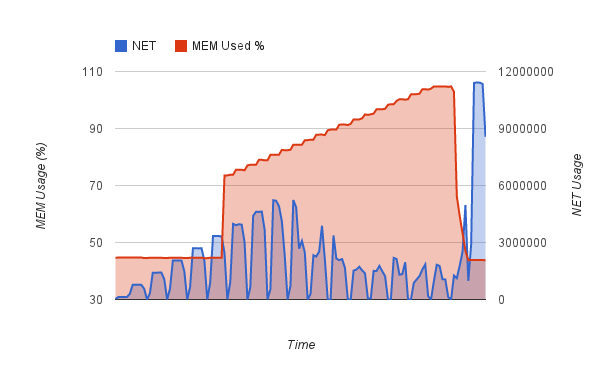
\includegraphics{MEM_NET-Problem.png}
\end{figure}
\begin{itemize}
\item {} 
When running an Emulation containing an Event based distribution, then the list of jobs (seen by using the command `ccmsh -j') may not be correct

\end{itemize}


\subsection{Adding a new emulator}
\label{COCOMA/09_adding_distributions_emulators::doc}\label{COCOMA/09_adding_distributions_emulators:adding-a-new-emulator}
In order to add a new emulator, a new wrapper has to be implemented. This needs to inherit from the relative abstract class, which can be found in the same \emph{emulators} directory. The class needs 3 different methods:
\begin{itemize}
\item {} 
\textbf{emulatorHelp}: Used for displaying help about an emulator (eg. what parameters it needs)

\item {} 
\textbf{emulatorArgNames}: Used for returning the names of the arguments that a given emulator takes

\end{itemize}

Specific methods to execute the wanted emulator instance with the relative needed parameters will have to be added. Checking the existing emulator wrappers should give a clear view on how the wrapping process can be carried out.


\subsection{Adding a new distribution}
\label{COCOMA/09_adding_distributions_emulators:adding-a-new-distribution}
In order to add a new distribution, it needs to inherit from the relative abstract class, which can be found in the same \emph{distributions} directory. The class needs 3 different methods:
\begin{itemize}
\item {} 
\textbf{distHelp}: Used for displaying help about a distribution (eg. what Resources types it can use)

\item {} 
\textbf{functionCount}: Used for getting values for: stressValues, runStartTimeList, runDurations. The actual algorithm (which calculates those values) goes in this function

\item {} 
\textbf{argNames}: Used for returning the names of the arguments that a given resource takes

\end{itemize}


\subsection{Additional Features}
\label{COCOMA/06_additional_features::doc}\label{COCOMA/06_additional_features:additional-features}
In this section the additional features of COCOMA will be discussed


\subsubsection{Testing}
\label{COCOMA/06_additional_features:testing}
COCOMA has two main sets of tests supplied with it; \textbf{API Tests} and \textbf{Command Line Interface (CLI) Tests}. Both of which are implemented using python's unit testing framework (pyUnit)

The test files (\textbf{TestAPI} and \textbf{TestCLI}) are located in \emph{``/usr/share/pyshared/cocoma/unitTest''}

To run a set of tests on the API or CLI, navigate to the \emph{unitTest} folder and use on of the commands:

\begin{Verbatim}[commandchars=\\\{\}]
\PYG{n+nv}{\PYGZdl{} }python \PYGZhy{}m unittest \PYGZhy{}v TestAPI
\PYG{n+nv}{\PYGZdl{} }python \PYGZhy{}m unittest \PYGZhy{}v TestCLI
\end{Verbatim}

The \emph{-v} argument gives more verbose output, and may be omitted if required

Individual test results are output to the terminal in the format \code{test\_Emulators (TestAPI.TestAPI) ... ok} if the test was successful
An unsuccessful test will produce the same outoput, with \emph{ERROR} or \emph{FAIL} instead of \emph{ok}

Once all the tests in the  file have run, a summary of the results will be printed. This will indicate which (if any) tests were unsuccessful, and attempt to give a reason why the test failed


\paragraph{CLI Testing}
\label{COCOMA/06_additional_features:cli-testing}
Individual tests can be run on the CLI using the syntax

\begin{Verbatim}[commandchars=\\\{\}]
\PYG{n+nv}{\PYGZdl{} }python \PYGZhy{}m unittest TestCLI.TestCLI.test\PYGZus{}Name
\end{Verbatim}

Where \code{test\_Name} is replaced by one of the following:

\begin{Verbatim}[commandchars=\\\{\}]
\PYG{n}{test\PYGZus{}EMU\PYGZus{}CPU}
\PYG{n}{test\PYGZus{}EMU\PYGZus{}IO}
\PYG{n}{test\PYGZus{}EMU\PYGZus{}IOTrap}
\PYG{n}{test\PYGZus{}EMU\PYGZus{}MEM}
\PYG{n}{test\PYGZus{}EMU\PYGZus{}MEMTrap}
\PYG{n}{test\PYGZus{}EMU\PYGZus{}MULTI1}
\PYG{n}{test\PYGZus{}EMU\PYGZus{}MULTI2}
\PYG{n}{test\PYGZus{}EMU\PYGZus{}NETWORK}
\PYG{n}{test\PYGZus{}EMU\PYGZus{}NowOperator}

\PYG{n}{test\PYGZus{}Scheduler\PYGZus{}Start}
\PYG{n}{test\PYGZus{}Scheduler\PYGZus{}Show}
\PYG{n}{test\PYGZus{}Scheduler\PYGZus{}Stop}

\PYG{n}{test\PYGZus{}API\PYGZus{}Start}
\PYG{n}{test\PYGZus{}API\PYGZus{}Show}
\PYG{n}{test\PYGZus{}API\PYGZus{}Stop}

\PYG{n}{test\PYGZus{}Help}
\PYG{n}{test\PYGZus{}Version}
\PYG{n}{test\PYGZus{}List}
\PYG{n}{test\PYGZus{}Result}
\PYG{n}{test\PYGZus{}Distributions}
\PYG{n}{test\PYGZus{}Emulators}
\PYG{n}{test\PYGZus{}Purge}
\PYG{n}{test\PYGZus{}Jobs}
\end{Verbatim}

This will produce output similar to running the entire set of tests


\paragraph{API Testing}
\label{COCOMA/06_additional_features:api-testing}
Individual tests can be run on the API using the syntax

\begin{Verbatim}[commandchars=\\\{\}]
\PYG{n+nv}{\PYGZdl{} }python \PYGZhy{}m unittest TestAPI.TestAPI.test\PYGZus{}Name
\end{Verbatim}

Where \code{test\_Name} is replaced by one of the following:

\begin{Verbatim}[commandchars=\\\{\}]
\PYG{n}{test\PYGZus{}List\PYGZus{}Emulation}
\PYG{n}{test\PYGZus{}List\PYGZus{}Emulator}
\PYG{n}{test\PYGZus{}List\PYGZus{}Distributions}
\PYG{n}{test\PYGZus{}List\PYGZus{}Results}
\PYG{n}{test\PYGZus{}List\PYGZus{}Logs}
\PYG{n}{test\PYGZus{}List\PYGZus{}SysLogs}
\PYG{n}{test\PYGZus{}List\PYGZus{}EmuLogs}
\PYG{n}{test\PYGZus{}List\PYGZus{}Tests}

\PYG{n}{test\PYGZus{}EMU\PYGZus{}Logs}
\PYG{n}{test\PYGZus{}EMUcr\PYGZus{}IO}
\PYG{n}{test\PYGZus{}EMUcr\PYGZus{}IOtrap}
\PYG{n}{test\PYGZus{}EMUcr\PYGZus{}MEM}
\PYG{n}{test\PYGZus{}EMUcr\PYGZus{}MEMtrap}
\PYG{n}{test\PYGZus{}EMUcr\PYGZus{}NETWORK}
\PYG{n}{test\PYGZus{}EMUcr\PYGZus{}MULTI1}
\PYG{n}{test\PYGZus{}EMUcr\PYGZus{}MULTI2}
\end{Verbatim}

This will produce output similar to running the entire set of tests


\subsubsection{Resource Overloading}
\label{COCOMA/06_additional_features:resource-overloading}
In order to prevent resources from becoming Overloaded (using more than 100\% of a resource at a point in time,) the system calculates the resource usage before any Emulation is run.

If an Emulation would cause any of the resources to become overloaded, then that emulation will not run and an exception will be raised with the format:

\begin{Verbatim}[commandchars=\\\{\}]
Unable to create distribution:
CPU resource will become Overloaded: Stopping execution
\end{Verbatim}


\subsubsection{Abstract Classes}
\label{COCOMA/06_additional_features:abstract-classes}
When adding a new Emulator or Distribution class they should extend their respective abstract class. This requires the new class to contain the following code:
\begin{itemize}
\item {} 
For Emulators
\begin{quote}

\begin{Verbatim}[commandchars=\\\{\}]
sys.path.insert(0, getHomepath() + '/emulators/')
from abstract\_emu import *

class run\_yourEmulatorName(abstract\_emu):
pass
\end{Verbatim}
\end{quote}

\item {} 
For Distributions
\begin{quote}

\begin{Verbatim}[commandchars=\\\{\}]
sys.path.insert(0, getHomepath() + '/distributions/')
from abstract\_dist import *

class dist\_yourDistributionName(abstract\_dist):
pass
\end{Verbatim}
\end{quote}

\end{itemize}

This feature was added to minimize problems caused by adding new emulators or distributions


\subsubsection{Message queue use}
\label{COCOMA/06_additional_features:message-queue-use}
COCOMA writes messages to the EMQ, which are used by the provenance service. Each message contains a timestamp, the message content and the component that created it. The message contains further information as the type of action, and various parameters depending on the specific action. The format adopted is to have key starting in capital, and use the \emph{camel} notation in case of multi-words. Below is the set of messages:

\begin{Verbatim}[commandchars=\\\{\}]
\PYGZob{}"Timestamp": 1378893008.422242, "Message": \PYGZob{}"Action": "Scheduler started",
"Interface": "eth0", "Port": "51889"\PYGZcb{}, "From": "Scheduler"\PYGZcb{}

\PYGZob{}"Timestamp": 1378893809.897368, "Message": \PYGZob{}"Action": "USER REQUEST Create
Emulation", "File": "tests/02-MEM-Linear\_incr-Stressapptest\_100-1000.xml"\PYGZcb{},
"From": "ccmsh"\PYGZcb{}

\PYGZob{}"Timestamp": 1378893810.206373, "Message": \PYGZob{}"Action": "Emulation request
received", "UserEmulationName": "MEM\_EMU"\PYGZcb{}, "From": "Emulation Manager"\PYGZcb{}

\PYGZob{}"Timestamp": 1378893810.744948, "Message": \PYGZob{}"ResourceTypeDist": "mem",
"JobName": "2-MEM\_EMU-2-0-mem\_distro-lookbusy-mem", "DistributionName":
"mem\_distro", "Emulator": "lookbusy", "Action": "Job Created", "RunNo":
"0", "EndTime": "2013-09-11 10:04:31", "EmulationName": "2-MEM\_EMU",
"DistributionID": 2, "StressValue": 100, "StartTime": "2013-09-11 10:03:31",
"Duration": 60.0\PYGZcb{}, "From": "Scheduler"\PYGZcb{}

\PYGZob{}"Timestamp": 1378893811.128323, "Message": \PYGZob{}"ResourceTypeDist": "mem",
"JobName": "2-MEM\_EMU-2-1-mem\_distro-lookbusy-mem", "DistributionName":
"mem\_distro", "Emulator": "lookbusy", "Action": "Job Created", "RunNo":
"1", "EndTime": "2013-09-11 10:04:31", "EmulationName": "2-MEM\_EMU",
"DistributionID": 2, "StressValue": 75, "StartTime": "2013-09-11 10:03:43",
"Duration": 48.0\PYGZcb{}, "From": "Scheduler"\PYGZcb{}

\PYGZob{}"Timestamp": 1378893811.479812, "Message": \PYGZob{}"ResourceTypeDist": "mem",
"JobName": "2-MEM\_EMU-2-2-mem\_distro-lookbusy-mem", "DistributionName":
"mem\_distro", "Emulator": "lookbusy", "Action": "Job Created", "RunNo": "2",
"EndTime": "2013-09-11 10:04:31", "EmulationName": "2-MEM\_EMU",
"DistributionID": 2, "StressValue": 75, "StartTime": "2013-09-11 10:03:55",
"Duration": 36.0\PYGZcb{}, "From": "Scheduler"\PYGZcb{}

\PYGZob{}"Timestamp": 1378893811.838568, "Message": \PYGZob{}"ResourceTypeDist": "mem",
"JobName": "2-MEM\_EMU-2-3-mem\_distro-lookbusy-mem", "DistributionName":
"mem\_distro", "Emulator": "lookbusy", "Action": "Job Created", "RunNo":
"3", "EndTime": "2013-09-11 10:04:31", "EmulationName": "2-MEM\_EMU",
"DistributionID": 2, "StressValue": 75, "StartTime": "2013-09-11 10:04:07",
"Duration": 24.0\PYGZcb{}, "From": "Scheduler"\PYGZcb{}

\PYGZob{}"Timestamp": 1378893812.189469, "Message": \PYGZob{}"ResourceTypeDist": "mem",
"JobName": "2-MEM\_EMU-2-4-mem\_distro-lookbusy-mem", "DistributionName":
"mem\_distro", "Emulator": "lookbusy", "Action": "Job Created", "RunNo":
"4", "EndTime": "2013-09-11 10:04:31", "EmulationName": "2-MEM\_EMU",
"DistributionID": 2, "StressValue": 75, "StartTime": "2013-09-11 10:04:19",
"Duration": 12.0\PYGZcb{}, "From": "Scheduler"\PYGZcb{}

\PYGZob{}"Timestamp": 1378893812.621874, "Message": \PYGZob{}"Action": "Emulation created",
"EmulationName": "MEM\_EMU"\PYGZcb{}, "From": "Emulation Manager"\PYGZcb{}

\PYGZob{}"Timestamp": 1378893871.00535, "Message": \PYGZob{}"Action": "Emulation finished",
"EmulationName": "2-MEM\_EMU"\PYGZcb{}, "From": "Logger"\PYGZcb{}

\PYGZob{}"Timestamp": 1378893871.163372, "Message": \PYGZob{}"Action": "Job Executed Successfully",
"StartTime": "2013-09-11 10:04:07", "Duration": 24.0,
"EndTime": "2013-09-11 10:04:31", "StressValue": 75, "JobName":
"2-MEM\_EMU-2-3-mem\_distro-lookbusy-mem"\PYGZcb{}, "From": "Scheduler"\PYGZcb{}

\PYGZob{}"Timestamp": 1378893871.274156, "Message": \PYGZob{}"Action": "Job Executed Successfully",
"StartTime": "2013-09-11 10:04:19", "Duration": 12.0, "EndTime":
"2013-09-11 10:04:31", "StressValue": 75, "JobName":
"2-MEM\_EMU-2-4-mem\_distro-lookbusy-mem"\PYGZcb{}, "From": "Scheduler"\PYGZcb{}

\PYGZob{}"Timestamp": 1378893871.398665, "Message": \PYGZob{}"Action": "Job Executed Successfully",
"StartTime": "2013-09-11 10:03:55", "Duration": 36.0, "EndTime":
"2013-09-11 10:04:31", "StressValue": 75, "JobName":
"2-MEM\_EMU-2-2-mem\_distro-lookbusy-mem"\PYGZcb{}, "From": "Scheduler"\PYGZcb{}

\PYGZob{}"Timestamp": 1378893871.493218, "Message": \PYGZob{}"Action": "Job Executed Successfully",
"StartTime": "2013-09-11 10:03:43", "Duration": 48.0,
"EndTime": "2013-09-11 10:04:31", "StressValue": 75, "JobName":
"2-MEM\_EMU-2-1-mem\_distro-lookbusy-mem"\PYGZcb{}, "From": "Scheduler"\PYGZcb{}

\PYGZob{}"Timestamp": 1378893871.628944, "Message": \PYGZob{}"Action": "Job Executed Successfully",
"StartTime": "2013-09-11 10:03:31", "Duration": 60.0, "EndTime":
"2013-09-11 10:04:31", "StressValue": 100, "JobName":
"2-MEM\_EMU-2-0-mem\_distro-lookbusy-mem"\PYGZcb{}, "From": "Scheduler"\PYGZcb{}

\PYGZob{}"Timestamp": 1378893913.604134, "Message": \PYGZob{}"Action":
"USER REQUEST list all Emulations"\PYGZcb{}, "From": "ccmsh"\PYGZcb{}

\PYGZob{}"Timestamp": 1378893929.615051, "Message": \PYGZob{}"Action":
"USER REQUEST list Emulation", "EmulationName": "2-MEM\_EMU"\PYGZcb{}, "From": "ccmsh"\PYGZcb{}

\PYGZob{}"Timestamp": 1378894024.729127, "Message": \PYGZob{}"Action":
"USER REQUEST delete Emulation", "EmulationName": "2-MEM\_EMU"\PYGZcb{}, "From": "ccmsh"\PYGZcb{}

\PYGZob{}"Timestamp": 1378894042.969776, "Message": \PYGZob{}"Action":
"USER REQUEST purge all Emulations"\PYGZcb{}, "From": "ccmsh"\PYGZcb{}
\end{Verbatim}


\subsubsection{Real trace parse}
\label{COCOMA/06_additional_features:real-trace-parse}
This feature allows a user to create a distribution from a real trace file. The format of the trace file has to be as follow:

\begin{Verbatim}[commandchars=\\\{\}]
NCPUS 2
MEMTOTAL 2074448
TIMESTAMP 1378900076312
POLLFR 1
CPU\%    MEMUSED\%
2               34
2               34
2               34
2               34
\end{Verbatim}

The first 4 lines provide information about the machine the trace was recorded from. This allows to scale the usage to the machine that has to reply it. As it can be seen, for now only \textbf{CPU} and \textbf{MEM} are supported. In the future, \textbf{IO} and \textbf{NET} might be supported too.
Below is a xml snippet showing a new tag called \textbf{trace} which provides the path to the trace file from which the distribution \textbf{real\_trace} creates the runs:

\begin{Verbatim}[commandchars=\\\{\}]
\textless{}distributions \textgreater{}
        \textless{}name\textgreater{}realTrace\textless{}/name\textgreater{}
        \textless{}startTime\textgreater{}0\textless{}/startTime\textgreater{}
        \textless{}!--duration in seconds --\textgreater{}
        \textless{}duration\textgreater{}60\textless{}/duration\textgreater{}
        \textless{}granularity\textgreater{}1\textless{}/granularity\textgreater{}
        \textless{}distribution href="/distributions/real\_trace" name="real\_trace" /\textgreater{}
        \textless{}trace\textgreater{}/path/to/real-trace\_1.txt\textless{}/trace\textgreater{}
        \textless{}emulator href="/emulators/lookbusy" name="lookbusy" /\textgreater{}
        \textless{}emulator-params\textgreater{}
                \textless{}resourceType\textgreater{}MEM\textless{}/resourceType\textgreater{}
                \textless{}!--time between iterations in usec (default 1000)--\textgreater{}
                \textless{}malloclimit\textgreater{}4004\textless{}/malloclimit\textgreater{}
                \textless{}memSleep\textgreater{}0\textless{}/memSleep\textgreater{}
        \textless{}/emulator-params\textgreater{}
\textless{}/distributions\textgreater{}
\end{Verbatim}

The \textbf{duration} is not used as the actual duration is calculated from the trace itself. So if the emulation ends before the distribution, all jobs left (running and scheduled) will be stopped.

As the concept of distribution in COCOMA relates to a single resource (CPU, RAM, IO, NET), if a mixed (CPU and RAM) real trace emulation wanted to be performed, 2 distributions can be added in the xml, each targeting one of the resources, but having the same \emph{startTime} and \emph{trace}.


\paragraph{Recording a real trace}
\label{COCOMA/06_additional_features:recording-a-real-trace}
COCOMA ships with a script called \emph{rec\_res\_usage.sh} which can be used to create a trace file with CPU and MEM used. The script can get as option the recording frequency, which by default is 1 sec. As the script can be used also as a live monitoring tool, in order to save the data into a file, the output redirection should be uses, such as:

\begin{Verbatim}[commandchars=\\\{\}]
\$ rec\_res\_usage.sh 2 \textgreater{} trace\_file.txt
        this uses a polling time of 2 seconds

\$ timeout 30s rec\_res\_usage.sh 2 \textgreater{} trace\_file.txt
        this uses the command *timeout* in front of the script so that
        it will run for the specified (30 seconds) amount of time
\end{Verbatim}


\paragraph{Event-driven approach}
\label{COCOMA/06_additional_features:event-driven-approach}
COCOMA offers 2 different ways to manage events. One is time-based, where a distribution is run for a finite and known amount of time. In this case when having two time-based distributions, where the second one has to run right after the first one has finished, given that the duration of the distribution is explicetely specified, it is possible to calculate the exact ending time of the first distribution and therefore schedule the start of the second one accordingly. However, there might be cases that the duration of a distribution is not known, e.g. in malicious distributions. In this case, say for example that out of the two distributions that want to be run sequentially, the first one doesn't have a duration, it would be impossible to schedule the second one since the end time of the first one is unknown. Therefore, we introduced the event-driven approach, where the first one creates an end-job event that triggers the schedule of the second distribution. This allows to take into account these duration-less distribution. An example is in the xml snippet below:

\begin{Verbatim}[commandchars=\\\{\}]
\textless{}distributions\textgreater{}
        \textless{}name\textgreater{}Fuzzer\_Distro1\textless{}/name\textgreater{}
        \textless{}nextevent\textgreater{}Fuzzer\_Distro2\textless{}/nextevent\textgreater{}
        \textless{}!--duration in seconds --\textgreater{}
        \textless{}starttime\textgreater{}0\textless{}/starttime\textgreater{}
        \textless{}granularity\textgreater{}0\textless{}/granularity\textgreater{}
        \textless{}duration\textgreater{}0\textless{}/duration\textgreater{}
        \textless{}distribution href="/distributions/event" name="event" /\textgreater{}
        \textless{}emulator href="/emulators/backfuzz" name="backfuzz" /\textgreater{}

        \textless{}emulator-params\textgreater{}
                \textless{}resourceType\textgreater{}NET\textless{}/resourceType\textgreater{}
                \textless{}serverip\textgreater{}10.55.164.181\textless{}/serverip\textgreater{}
                \textless{}serverport\textgreater{}80\textless{}/serverport\textgreater{}
                \textless{}min\textgreater{}100\textless{}/min\textgreater{}
                \textless{}max\textgreater{}104\textless{}/max\textgreater{}
                \textless{}packettype\textgreater{}HTTP\textless{}/packettype\textgreater{}
                \textless{}timedelay\textgreater{}0\textless{}/timedelay\textgreater{}
                \textless{}salt\textgreater{}2\textless{}/salt\textgreater{}
        \textless{}/emulator-params\textgreater{}
\textless{}/distributions\textgreater{}

\textless{}distributions\textgreater{}
        \textless{}name\textgreater{}Fuzzer\_Distro2\textless{}/name\textgreater{}
        \textless{}!--duration in seconds --\textgreater{}
        \textless{}nextevent\textgreater{}Fuzzer\_Distro2\textless{}/nextevent\textgreater{}
        \textless{}starttime\textgreater{}0\textless{}/starttime\textgreater{}
        \textless{}granularity\textgreater{}0\textless{}/granularity\textgreater{}
        \textless{}duration\textgreater{}0\textless{}/duration\textgreater{}
        \textless{}distribution href="/distributions/event" name="event" /\textgreater{}
        \textless{}emulator href="/emulators/backfuzz" name="backfuzz" /\textgreater{}

        \textless{}emulator-params\textgreater{}
                \textless{}resourceType\textgreater{}NET\textless{}/resourceType\textgreater{}
                \textless{}serverip\textgreater{}10.55.164.181\textless{}/serverip\textgreater{}
                \textless{}serverport\textgreater{}22\textless{}/serverport\textgreater{}
                \textless{}min\textgreater{}100\textless{}/min\textgreater{}
                \textless{}max\textgreater{}104\textless{}/max\textgreater{}
                \textless{}packettype\textgreater{}SSH\textless{}/packettype\textgreater{}
                \textless{}timedelay\textgreater{}0\textless{}/timedelay\textgreater{}
                \textless{}salt\textgreater{}2\textless{}/salt\textgreater{}
        \textless{}/emulator-params\textgreater{}
\textless{}/distributions\textgreater{}
\end{Verbatim}

The new distribution format in this case has a new tag \textbf{nextevent}, which allows the scheduler to understand that the following distribution to be scheduled, once the first distribution finishes, is the one in this tag. The example relates to a malicious distribution, which is further explained in a dedicated section of this document. Please note that in this case, although they are specified, the \emph{starttime}, \emph{granularity} and \emph{duration} are not actually used as they don't apply in the event-driven context. Finally, the \emph{emustopTime} still sets the emulation ends, so in case a distribution hasn't finished within the emulation time range specified, the jobs left (running and scheduled) will be stopped.


\subsubsection{Malicious module}
\label{COCOMA/06_additional_features:malicious-module}
The malicious module allows users to create distributions that can target a specific machine by sending fuzzing data over a chosen protocol. As the emulator supporting our malicious module is \emph{backfuzz} \footnote{
\href{https://github.com/localh0t/backfuzz}{https://github.com/localh0t/backfuzz}
} \footnote{
\href{http://www.darknet.org.uk/2012/03/backfuzz-multi-protocol-fuzzing-toolkit-supports-httpftpimap-etc/}{http://www.darknet.org.uk/2012/03/backfuzz-multi-protocol-fuzzing-toolkit-supports-httpftpimap-etc/}
}, it offers fuzzing over various known protocol such as \emph{HTTP}, \emph{SSH}, \emph{FTP}, \emph{IMAP}, etc. The nice thing that all protocols are added to the tool as plugins, so if a new protocol wants to be tested, a new plugin for it can be created and added to the tool for the purpose.
The fuzzing process time cannot be known a priori as it depends from factors out of the user control, such as the network between COCOMA and the SuT to target. Therefore, the \textbf{event-driven} approach was introduced to support this. The xml snippet below (the same of the event-driven section) shows a maliciuos distribution using backfuzz:

\begin{Verbatim}[commandchars=\\\{\}]
\textless{}distributions\textgreater{}
        \textless{}name\textgreater{}Fuzzer\_Distro1\textless{}/name\textgreater{}
        \textless{}nextevent\textgreater{}Fuzzer\_Distro2\textless{}/nextevent\textgreater{}
        \textless{}!--duration in seconds --\textgreater{}
        \textless{}starttime\textgreater{}0\textless{}/starttime\textgreater{}
        \textless{}granularity\textgreater{}0\textless{}/granularity\textgreater{}
        \textless{}duration\textgreater{}0\textless{}/duration\textgreater{}
        \textless{}distribution href="/distributions/event" name="event" /\textgreater{}
        \textless{}emulator href="/emulators/backfuzz" name="backfuzz" /\textgreater{}

        \textless{}emulator-params\textgreater{}
                \textless{}resourceType\textgreater{}NET\textless{}/resourceType\textgreater{}
                \textless{}serverip\textgreater{}10.55.164.181\textless{}/serverip\textgreater{}
                \textless{}serverport\textgreater{}80\textless{}/serverport\textgreater{}
                \textless{}min\textgreater{}100\textless{}/min\textgreater{}
                \textless{}max\textgreater{}104\textless{}/max\textgreater{}
                \textless{}packettype\textgreater{}HTTP\textless{}/packettype\textgreater{}
                \textless{}timedelay\textgreater{}0\textless{}/timedelay\textgreater{}
                \textless{}salt\textgreater{}2\textless{}/salt\textgreater{}
        \textless{}/emulator-params\textgreater{}
\textless{}/distributions\textgreater{}
\end{Verbatim}

In the emulator parameters part we can specify the server IP and its port, the minimum and maximum lenght of the fuzzing string sent, the type of protocol and the time after which the fuzz starts.


\subsection{Known Issues}
\label{COCOMA/08_known_issues:known-issues}\label{COCOMA/08_known_issues::doc}
The interaction of the various emulators used in COCOMA can cause unexpected issues. Some of these issues are listed below (This is \emph{not} an exhaustive list, and will be updated as new issues are discovered)
\begin{itemize}
\item {} 
Stressapptest uses \textasciitilde{}100\% CPU, regardless of what resource it is being ran on.

\item {} 
If a Linear increase distribution is run on memory using stressapptest at the same time as Iperf is being used to load the Network, then the Network resource may not reach its target load. This problem is usually encountered when the memory usage reaches over \textasciitilde{}80\% (as shown in the graph below)

\end{itemize}
\begin{figure}[htbp]
\centering

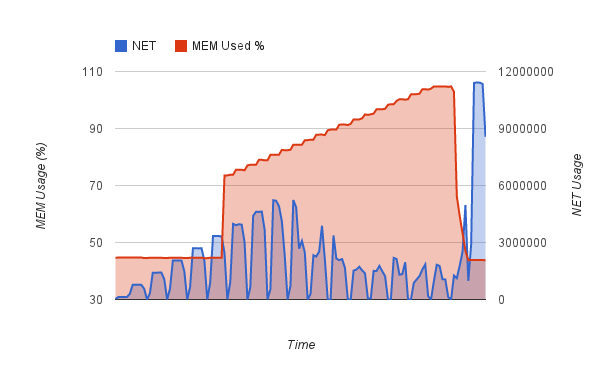
\includegraphics{MEM_NET-Problem.png}
\end{figure}
\begin{itemize}
\item {} 
When running an Emulation containing an Event based distribution, then the list of jobs (seen by using the command `ccmsh -j') may not be correct

\end{itemize}


\subsection{Implementation details}
\label{COCOMA/10_implementation_details:implementation-details}\label{COCOMA/10_implementation_details::doc}
The Controlled Contentious and Malicious patterns (COCOMA) framework aims to provide experimenters the ability to create specific contentious and malicious payloads and workloads in a controlled fashion. The experimenter is able to use pre-defined common distributions or specify new payloads and workloads. In the table below we present the terminology introduced by COCOMA.

\begin{tabulary}{\linewidth}{|p{4.5cm}|p{8.5cm}|}
\hline
\textbf{\relax 
Term
} & \textbf{\relax 
Description
}\\\hline

Emulation
 & 
Process that imitates a specific behaviour specified in the emulation type, over a resource type, using one or more distributions during the emulation lifetime
\\\hline

Emulation type
 & 
An emulation can be of the following types:
\begin{itemize}
\item {} 
Contentiousness

\item {} 
Maliciousness

\item {} 
Faultiness (not yet implemented)

\item {} 
Mixed (a combination of the above types)

\end{itemize}
\\\hline

Resource type
 & 
A resource can be of the following types:
\begin{itemize}
\item {} 
CPU

\item {} 
RAM

\item {} 
I/O

\item {} 
Network

\end{itemize}
\\\hline

Emulator
 & 
Specific mechanism/tool that is used to create an emulation type. For example load generators, stress generators, fault generators and malicious payload creation.
\\\hline

Distribution
 & 
In the case of contention, it is a discrete function of a specific resource type over a specific time within the emulation lifetime. The distribution time is divided into multiple timeslots (t0, .. , tn) based on the distribution granularity. A distribution is broken down into multiple runs each one injecting a different load level per time slot depending on the discrete function of the distribution. In the case of malicious, it is a straight mapping to the emulator
\\\hline

Distribution granularity
 & 
Number of runs for the distribution
\\\hline

Emulation lifetime
 & 
Duration of the emulation
\\\hline

Run
 & 
Basic emulator instantiation
\\\hline
\end{tabulary}


When a user defines an emulation, he needs to specify pairs of distribution-emulator. When specifying an emulator it is bound to a specific resource type. For more complex scenarios users can specify multiple pairs which can also overlap from the time point of view.

COCOMA is provided within a BonFIRE VM, which is interfaced with the BonFIRE aggregator as shown in the figure below:
\begin{figure}[htbp]
\centering
\capstart

\scalebox{0.800000}{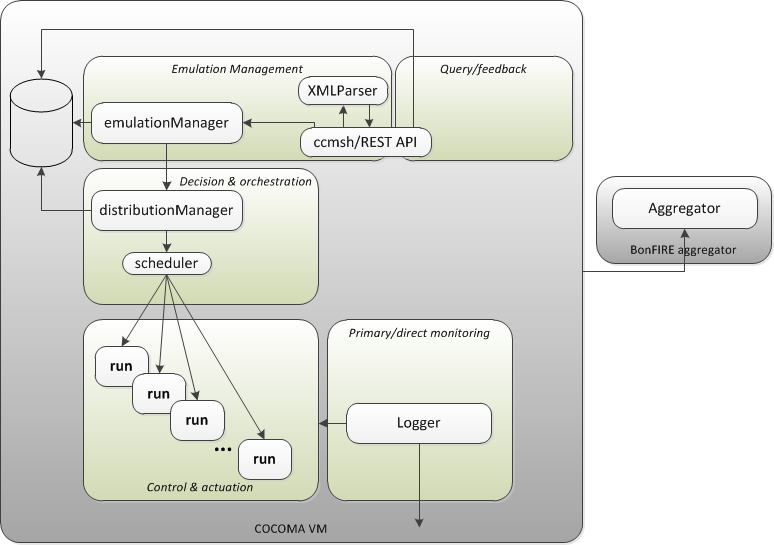
\includegraphics{cocoma-design.png}}
\caption{COCOMA design and components interactions}\label{COCOMA/10_implementation_details:cocoma-design}\end{figure}

The different functions provided by the COCOMA components and their interactions are explained below:
\begin{itemize}
\item {} 
\textbf{ccmsh}: this is the command line interface (CLI) to interact with COCOMA. Users can specify an emulation in an XML file, which is interpreted by the \emph{XMLParser} component. Also, the CLI allows to check and control the current running emulations (list, delete, etc.) by interacting directly with the DB

\item {} 
\textbf{REST API}: COCOMA provides also a REST API to interact with the framework programmatically

\item {} 
\textbf{XMLParser}: it checks xml correct format and return interpreted values to create an emulation. It is used by both \emph{CLI} and \emph{API}

\item {} 
\textbf{emulationManager}: the \emph{emulationManager} receives input from the ccmsh or the REST API to create/query/delete an emulation

\item {} 
\textbf{distributionManager}: the \emph{distributionManager} receives input from the \emph{emulationManager} to load the distribution(s) and apply the relative algorithm in the distribution(s). It basically calculates how many runs (individual basic emulator instances) are needed, and the parameters values of each run.  These are then passed to the \emph{scheduler}

\item {} 
\textbf{scheduler}: it creates the runs using the values obtained from the \emph{distributionManager} at due time

\item {} 
\textbf{DB}: it holds information about running emulations, registered emulators, distributions and some configurations

\item {} 
\textbf{Logger}: it creates 2 different log files, one with all events relative to the runs created and the other one with the resource usage

\end{itemize}

COCOMA is designed to work with different emulators. To add a new emulator a user needs to install the new emulator where COCOMA is installed, create a python wrapper for the specific parameters of the emulator and place this wrapper into the \emph{emulators} COCOMA directory. A similar approach is for distributions. Users can specify their desired discrete functions in a python file and place it in the \emph{distributions} directory. Emulators and distributions that are in the those directories are automatically available to be used. In the next sections we provide details of how to create both emulators and distributions.


\subsubsection{Code structure}
\label{COCOMA/10_implementation_details:code-structure}
COCOMA code structure is shown below:

\begin{Verbatim}[commandchars=\\\{\}]
/bin
/data
/distributions
/doc
/emulators
/logs
/rb-examples
/scripts
/tests
/unitTest
\_\_init\_\_.py
LICENSE
NEWS
NOTICE
README
\end{Verbatim}

The bin directory contains the main components presented in the {\hyperref[COCOMA/10_implementation_details:cocoma-design]{\emph{COCOMA design and components interactions}}} figure. It also contains 3 more files
\begin{itemize}
\item {} 
\emph{Job.py}: used to create and manage the \emph{scheduler} jobs

\item {} 
\emph{Library.py}: contains the common functions used by various components

\item {} 
\emph{Logger.py}: implements the logging mechanisms

\end{itemize}

The \emph{webUI} files are also contained within the \emph{bin} directory, specifically in a subdirectory called \emph{webcontent}.

The \emph{data} folder contains the SQLite database file. The \emph{distributions} directory contains the distributions currently available, while the emulators wrappers are in the \emph{emulators} folder. In the \emph{rb-examples} there are \emph{restufully} examples to create emulations using the \emph{COCOMA API}. In the \emph{scripts} directory there is the \emph{rec\_res\_usage} script that can be used to record a real trace from a system and replayed in COCOMA. Example xml tests are in the \emph{tests} directory, while the automated tests are in the \emph{unitTest} folder.


\subsubsection{Building process}
\label{COCOMA/10_implementation_details:building-process}
COCOMA is implemented in \emph{python}, while the \emph{webUI} in \emph{Javascripts}, therefore there is no need for building anything. On the other hand a deb package has been created to install the software along with some of the dependencies. A building script is provided along with the debian files (\emph{control}, \emph{postinst} and \emph{postrm}). The script uses 4 specific commands in order:
\begin{itemize}
\item {} 
\emph{sdist}: this is used by python \code{python setup.py sdist} to create a python source distribution as \emph{tar.gz} file format \footnote{
\href{http://docs.python.org/distutils/sourcedist.html}{http://docs.python.org/distutils/sourcedist.html}
}. In order to use the command, a \emph{setup.py} is provided as well \footnote{
\href{http://docs.python.org/2/distutils/setupscript.html}{http://docs.python.org/2/distutils/setupscript.html}
}. To use the \emph{setuptools} in the \emph{setup.py}, a \emph{distribute\_setup.py} is also needed. This is provided too

\item {} 
\emph{py2dsc}: this generates a debian source package from a Python package \footnote{
\href{https://pypi.python.org/pypi/stdeb}{https://pypi.python.org/pypi/stdeb}
}

\item {} 
\emph{dch}: this adds a new revision at the top of the Debian changelog file \footnote{
\href{http://www.debian.org/doc/manuals/maint-guide/update.en.html}{http://www.debian.org/doc/manuals/maint-guide/update.en.html}
}

\item {} 
\emph{debuild}: this buils the debian package \footnote{
\href{http://www.debian.org/doc/manuals/maint-guide/build.en.html}{http://www.debian.org/doc/manuals/maint-guide/build.en.html}
}

\end{itemize}

The building script pulls the cocoma source code from the \emph{github} repository \footnote{
\href{https://github.com/cragusa/cocoma}{https://github.com/cragusa/cocoma}
}. It takes as argument the version of the debian package that one wants to built such as:

\begin{Verbatim}[commandchars=\\\{\}]
./build\_cocoma-deb 1.7.4
\end{Verbatim}

The building script, along the other needed python scripts (setup.py, distribute\_setup.py) and the directory structure needed can be found in the BonFIRE svn repository \footnote{
\href{https://scm.gforge.inria.fr/svn/bonfire-dev/cocoma/build-deb/}{https://scm.gforge.inria.fr/svn/bonfire-dev/cocoma/build-deb/}
}. Once the directory is checked out, the script can be run from that directory and the deb package will be created in the \code{dist/deb\_dist} folder.


\subsubsection{Dependencies and other tools}
\label{COCOMA/10_implementation_details:dependencies-and-other-tools}
In order for COCOMA to work as required, a number of dependencies and tools are needed. Dependecies are:
\begin{itemize}
\item {} 
\textbf{python} version is \textbf{v2.7x}. Version v3.x hasn't been tested. \emph{python-support} and \emph{python-dev} are also needed

\item {} \begin{description}
\item[{\textbf{python modules} used by the componenents to implement various functionalities}] \leavevmode\begin{itemize}
\item {} 
\textbf{bottle}: \emph{is a fast, simple and lightweight WSGI micro web-framework}. Latest tested version is \textbf{v0.11.6}

\item {} 
\textbf{psutil}: \emph{is a module providing an interface for retrieving information on all running processes and system utilization (CPU, memory, disks, network)}. Latest tested version is \textbf{v1.0.1}

\item {} 
\textbf{pyro4}: \emph{it is a library that enables you to build applications in which objects can talk to eachother over the network}. Working tested version is \textbf{v4.20} is required. Later versions give serialization problems for the scheduler. This is a known issue by the pyro developers. If fixed, later versions should work

\item {} 
\textbf{apscheduler}: \emph{is a light but powerful in-process task scheduler that lets you schedule functions (or any other python callables) to be executed at times of your choosing}. Latest tested version is \textbf{v2.1.1}

\item {} 
\textbf{pika}: \emph{is a pure-Python implementation of the AMQP 0-9-1 protocol}. Latest tested version is \textbf{v0.9.13}

\item {} 
\textbf{PyUnit}: \emph{Python language version of unit testing framework JUnit}. Latest tested version is \textbf{v1.4.1}

\item {} 
\textbf{requests}: \emph{it is a HTTP library}. Latest tested version is \textbf{v2.0.0}

\item {} 
\textbf{numpy}: \emph{is a general-purpose array-processing package designed to efficiently manipulate large multi-dimensional arrays of arbitrary records}. Latest tested version is \textbf{v1.7.1}

\end{itemize}

\end{description}

\item {} 
\textbf{pip}: \emph{A tool for installing and managing Python packages}

\end{itemize}

As tools, COCOMA uses some as emulators, such as \emph{stressapptest} \footnote{
\href{https://code.google.com/p/stressapptest/}{https://code.google.com/p/stressapptest/}
}, \emph{lookbusy} \footnote{
\href{http://devin.com/lookbusy/}{http://devin.com/lookbusy/}
}, \emph{backfuzz} \footnote{
\href{https://github.com/localh0t/backfuzz}{https://github.com/localh0t/backfuzz}
} \footnote{
\href{http://www.darknet.org.uk/2012/03/backfuzz-multi-protocol-fuzzing-toolkit-supports-httpftpimap-etc/}{http://www.darknet.org.uk/2012/03/backfuzz-multi-protocol-fuzzing-toolkit-supports-httpftpimap-etc/}
}, \emph{iperf} \footnote{
\href{https://code.google.com/p/iperf/}{https://code.google.com/p/iperf/}
}. Other used tools are for installation, such as \code{curl, bc, unzip, gcc, g++, make}.


\section{Indices and tables}
\label{index:indices-and-tables}\begin{itemize}
\item {} 
\emph{genindex}

\end{itemize}
\begin{itemize}
\item {} 
Glossary

\end{itemize}



\renewcommand{\indexname}{Index}
\printindex
\end{document}
